% Created 2014-06-24 Tue 15:36
\documentclass[bigger]{beamer}
\usepackage[utf8]{inputenc}
\usepackage[T1]{fontenc}
\usepackage{fixltx2e}
\usepackage{graphicx}
\usepackage{longtable}
\usepackage{float}
\usepackage{wrapfig}
\usepackage{soul}
\usepackage{textcomp}
\usepackage{marvosym}
\usepackage{wasysym}
\usepackage{latexsym}
\usepackage{amssymb}
\usepackage{hyperref}
\tolerance=1000
\mode<beamer>{\usetheme[compress]{Berlin}}
\usepackage{graphicx}
\usepackage{amsmath}
\usepackage{lmodern}
\usepackage{ifmtarg}
\usepackage{tikz}
\usetikzlibrary{calc}
\makeatletter
\newcommand\ChangeItemFont[3]{%
\renewcommand{\itemize}[1][]{%
  \beamer@ifempty{##1}{}{\def\beamer@defaultospec{#1}}%
  \ifnum \@itemdepth >2\relax\@toodeep\else
    \advance\@itemdepth\@ne
    \beamer@computepref\@itemdepth% sets \beameritemnestingprefix
    \usebeamerfont{itemize/enumerate \beameritemnestingprefix body}%
    \usebeamercolor[fg]{itemize/enumerate \beameritemnestingprefix body}%
    \usebeamertemplate{itemize/enumerate \beameritemnestingprefix body begin}%
    \list
      {\usebeamertemplate{itemize \beameritemnestingprefix item}}
      {\def\makelabel####1{%
          {%
            \hss\llap{{%
                \usebeamerfont*{itemize \beameritemnestingprefix item}%
                \usebeamercolor[fg]{itemize \beameritemnestingprefix item}####1}}%
          }%
        }%
  \ifnum\@itemdepth=1\relax
    #1%
  \else
  \ifnum\@itemdepth=2\relax
    #2%
  \else
  \ifnum\@itemdepth=3\relax
    #3%
  \fi%
  \fi%
  \fi%
  }
  \fi%
  \beamer@cramped%
  \raggedright%
  \beamer@firstlineitemizeunskip%
}}
\makeatother

\setbeamertemplate{footline}
  {%
    \begin{beamercolorbox}[colsep=1.5pt]{upper separation line foot}
    \end{beamercolorbox}
    \begin{beamercolorbox}[ht=2.5ex,dp=1.125ex,%
      leftskip=.3cm,rightskip=.3cm plus1fil]{author in head/foot}%
      \leavevmode{\usebeamerfont{author in head/foot}\insertshortauthor}%
      \hfill%
      {\usebeamerfont{institute in head/foot}\usebeamercolor[fg]{institute in head/foot}\insertshortinstitute}%
    \end{beamercolorbox}%
    \begin{beamercolorbox}[ht=2.5ex,dp=1.125ex,%
      leftskip=.3cm,rightskip=.3cm plus1fil]{title in head/foot}%
      {\usebeamerfont{title in head/foot}\insertshorttitle}%
      \hfill%
      {\usebeamerfont{frame number}\usebeamercolor[fg]{frame number}\insertframenumber~/~\inserttotalframenumber}
    \end{beamercolorbox}%
    \begin{beamercolorbox}[colsep=1.5pt]{lower separation line foot}
    \end{beamercolorbox}
  }
\makeatother


%----------------------------------------------------------------------
% Define useful commands
%----------------------------------------------------------------------

\newcommand{\eejj}{\ensuremath{eejj} }
\newcommand{\enujj}{\ensuremath{e\nu jj} }
\newcommand{\mumujj}{\ensuremath{\mu\mu jj} }
\newcommand{\munujj}{\ensuremath{\mu\nu jj} }
\newcommand{\emujj}{\ensuremath{e\mu jj} }
\newcommand{\zjets}{\ensuremath{\text{Z}^{0}}+jets }
\newcommand{\wjets}{\ensuremath{\text{W}^{\pm}}+jets }
\newcommand{\ttbar}{\ensuremath{t\bar{t}} }

\newcommand{\pt}{\ensuremath{p_{\text{T}}} }
\newcommand{\ST}{\ensuremath{S_{\text{T}}} }
\newcommand{\mee}{\ensuremath{m_{\text{ee}}} }
\newcommand{\mll}{\ensuremath{m_{\ell\ell}} }
\newcommand{\mej}{\ensuremath{m_{\text{ej}}} }
\newcommand{\mejmin}{\ensuremath{m_{\text{ej}}^{\text{min}}} }
\newcommand{\mejavg}{\ensuremath{m_{\text{ej}}^{\text{avg}}} }
% \newcommand{\mt}{\ensuremath{m_{\text{T, e}\nu}}}
\newcommand{\mtjnu}{\ensuremath{m_{\text{T, j}\nu}} }


\newcommand{\met}{\ensuremath{\not\!\!{E_{\text{T}}}} }
\newcommand{\mt}{\ensuremath{m_{\text{T, e}\nu}} }

%----------------------------------------------------------------------
% Define useful numbers
%----------------------------------------------------------------------

% Lumi info
\newcommand{\intLumi}{$19.6 \text{ fb}^{-1}$}

% MC scale factors
\newcommand{\enujjWJetsMonteCarloScaleFactor}{0.85 \pm 0.01 \text{ (stat)} \pm 0.01    \text{ (syst)}}
\newcommand{\enujjTTBarMonteCarloScaleFactor}{0.97 \pm 0.02 \text{ (stat)} \pm 0.01    \text{ (syst)}}
% \newcommand{\eejjZJetsMonteCarloScaleFactor} {0.97 \pm 0.01 \text{ (stat)} \pm 0.00004 \text{ (syst)}}
\newcommand{\eejjZJetsMonteCarloScaleFactor} {0.97 \pm 0.01 \text{ (stat)}}

\newcommand{\enujjWJetsMonteCarloScaleFactorMETRescaled}{0.95 \pm 0.02 \text{ (stat)} \pm 0.01 \text{ (syst)}}
\newcommand{\enujjTTBarMonteCarloScaleFactorMETRescaled}{1.07 \pm 0.03 \text{ (stat)} \pm 0.01 \text{ (syst)}}

\newcommand{\enujjWJetsMonteCarloScaleFactorMETandMTRescaled}{0.97 \pm 0.02 \text{ (stat)} \pm 0.01 \text{ (syst)}}
\newcommand{\enujjTTBarMonteCarloScaleFactorMETandMTRescaled}{1.08 \pm 0.03 \text{ (stat)} \pm 0.01 \text{ (syst)}}

\newcommand{\eejjZControlRegionContamination}{4\%}

% Electron scale factors
\newcommand{\electronRecoDataMCScaleFactor}{0.98}
\newcommand{\electronRecoDataMCScaleFactorRelUnc}{1.5}
\newcommand{\electronRecoDataMCScaleFactorSqr}{0.96}

% GEN-level cross-sections (not yet rescaled) 
\newcommand{\wjetsXSection}{37509.0 pb}
\newcommand{\zjetsXSection}{3503.71 pb}
\newcommand{\ttbarXSection}{234 pb}
\newcommand{\stopSChannelXSection}{5.55 pb}
\newcommand{\stopTChannelXSection}{87.1 pb}
\newcommand{\stopTWChannelXSection}{22.2 pb}
\newcommand{\wwXSection}{57.1 pb} % THESE NEED TO BE UPDATED!!!
\newcommand{\wzXSection}{32.3 pb} % THESE NEED TO BE UPDATED!!!
\newcommand{\zzXSection}{8.26 pb} % THESE NEED TO BE UPDATED!!!

% QCD contributions at limit of the analysis
\newcommand{\percentQCDatEEJJLimit}{1\%}
\newcommand{\percentQCDatENuJJLimit}{3\%}

% Closure test contamination
\newcommand{\percentContaminationClosureTest}{5\%}
\newcommand{\percentContaminationClosureTestFinal}{55\%}

% Closure test (low-ST) results
\newcommand{\closureTestLowSTPredicted}{13100}
\newcommand{\closureTestLowSTPredictedUnc}{400}
\newcommand{\closureTestLowSTObserved}{12100}
\newcommand{\closureTestLowSTObservedUnc}{400}
\newcommand{\closureTestLowSTRatio}{1.08}
\newcommand{\closureTestLowSTRatioUnc}{0.05}

% Closure test (mid-ST) results
\newcommand{\closureTestMidSTPredicted}{877}
\newcommand{\closureTestMidSTPredictedUnc}{46.7}
\newcommand{\closureTestMidSTObserved}{600}
\newcommand{\closureTestMidSTObservedUnc}{53}
\newcommand{\closureTestMidSTRatio}{1.46}
\newcommand{\closureTestMidSTRatioUnc}{0.15}

% QCD systematic uncertainty
\newcommand{\qcdSystematicUncertaintyPerEle}{30\%}
\newcommand{\qcdSystematicUncertaintyTwoEle}{60\%}

% TTbar (e-mu-jj) contamination
\newcommand{\emujjContamination}{2\%}
\newcommand{\emujjRecoScaleFactor}{0.974  \pm 0.011 \text{ (stat)}}

% mumujj/munujj scale factors for data-driven background
\newcommand{\mumujjRecoScaleFactor}{97.5 \pm 0.4 \text{ (stat)}}
\newcommand{\munujjRecoScaleFactor}{97.2 \pm 0.5 \text{ (stat)}}

% Shape uncertainties
\newcommand{\enujjWJetsShapeUncertainty}{5.92\%}
\newcommand{\enujjTTBarShapeUncertainty}{8.17\%}
\newcommand{\eejjZJetsShapeUncertainty}{8.70\%}

% EES uncertainties
\newcommand{\electronEnergyScaleUncBarrel}{0.4\%}
\newcommand{\electronEnergyScaleUncEndcap}{4.1\%}

% EER uncertainties
\newcommand{\electronEnergyResolutionUncBarrel}{1.006}
\newcommand{\electronEnergyResolutionUncEndcap}{1.015}

% lumi uncertainty
\newcommand{\lumiUncertainty}{2.6\%}

% limits
\newcommand{\eejjObservedLimit}{1005}
\newcommand{\eejjExpectedLimit}{1030}
\newcommand{\enujjObservedLimit}{845}
\newcommand{\enujjExpectedLimit}{890}

\newcommand{\enujjObservedLimitCombined}{845}
\newcommand{\enujjExpectedLimitCombined}{932}

\newcommand{\eejjObservedLimitNoSyst}{1010}
\newcommand{\eejjExpectedLimitNoSyst}{1030}
\newcommand{\enujjObservedLimitNoSyst}{850}
\newcommand{\enujjExpectedLimitNoSyst}{895}

\newcommand{\eejjObservedLimitMuon}{1015}
\newcommand{\eejjExpectedLimitMuon}{980}
\newcommand{\enujjObservedLimitMuon}{825}
\newcommand{\enujjExpectedLimitMuon}{890}


\newcommand{\lowBetaExpectedLimit}{790}
\newcommand{\lowBetaObservedLimit}{635}

\mode<beamer>{\usecolortheme{bear}}
\mode<beamer>{\titlegraphic{\includegraphics[width=0.2\textwidth]{brown-logo}}}
\institute[Brown University]{\inst{1} Brown University \and \inst{2} University of Alabama \and \inst{3} Rome}
\providecommand{\alert}[1]{\textbf{#1}}

\title{EXO-12-041 Approval [Backup]}
\author{Edmund Berry}
\date{Tuesday, June 24, 2014}
\hypersetup{
  pdfkeywords={},
  pdfsubject={},
  pdfcreator={Emacs Org-mode version 7.8.11}}

\author[Edmund Berry]{\alert{E. Berry}\inst{1}, S. Cooper\inst{2}, P. Rumerio\inst{2}, F. Santanastasio\inst{3}}
\begin{document}

\maketitle

\section{Backup}
\label{sec-1}
\subsection{\eejj preselection}
\label{sec-1-1}
\begin{frame}
\frametitle{\eejj preselection: electron \pt}
\label{sec-1-1-1}
\begin{columns}
\begin{column}{0.6\textwidth}
%% 1st electron pt
\label{sec-1-1-1-1}

\centering
Leading electron \pt
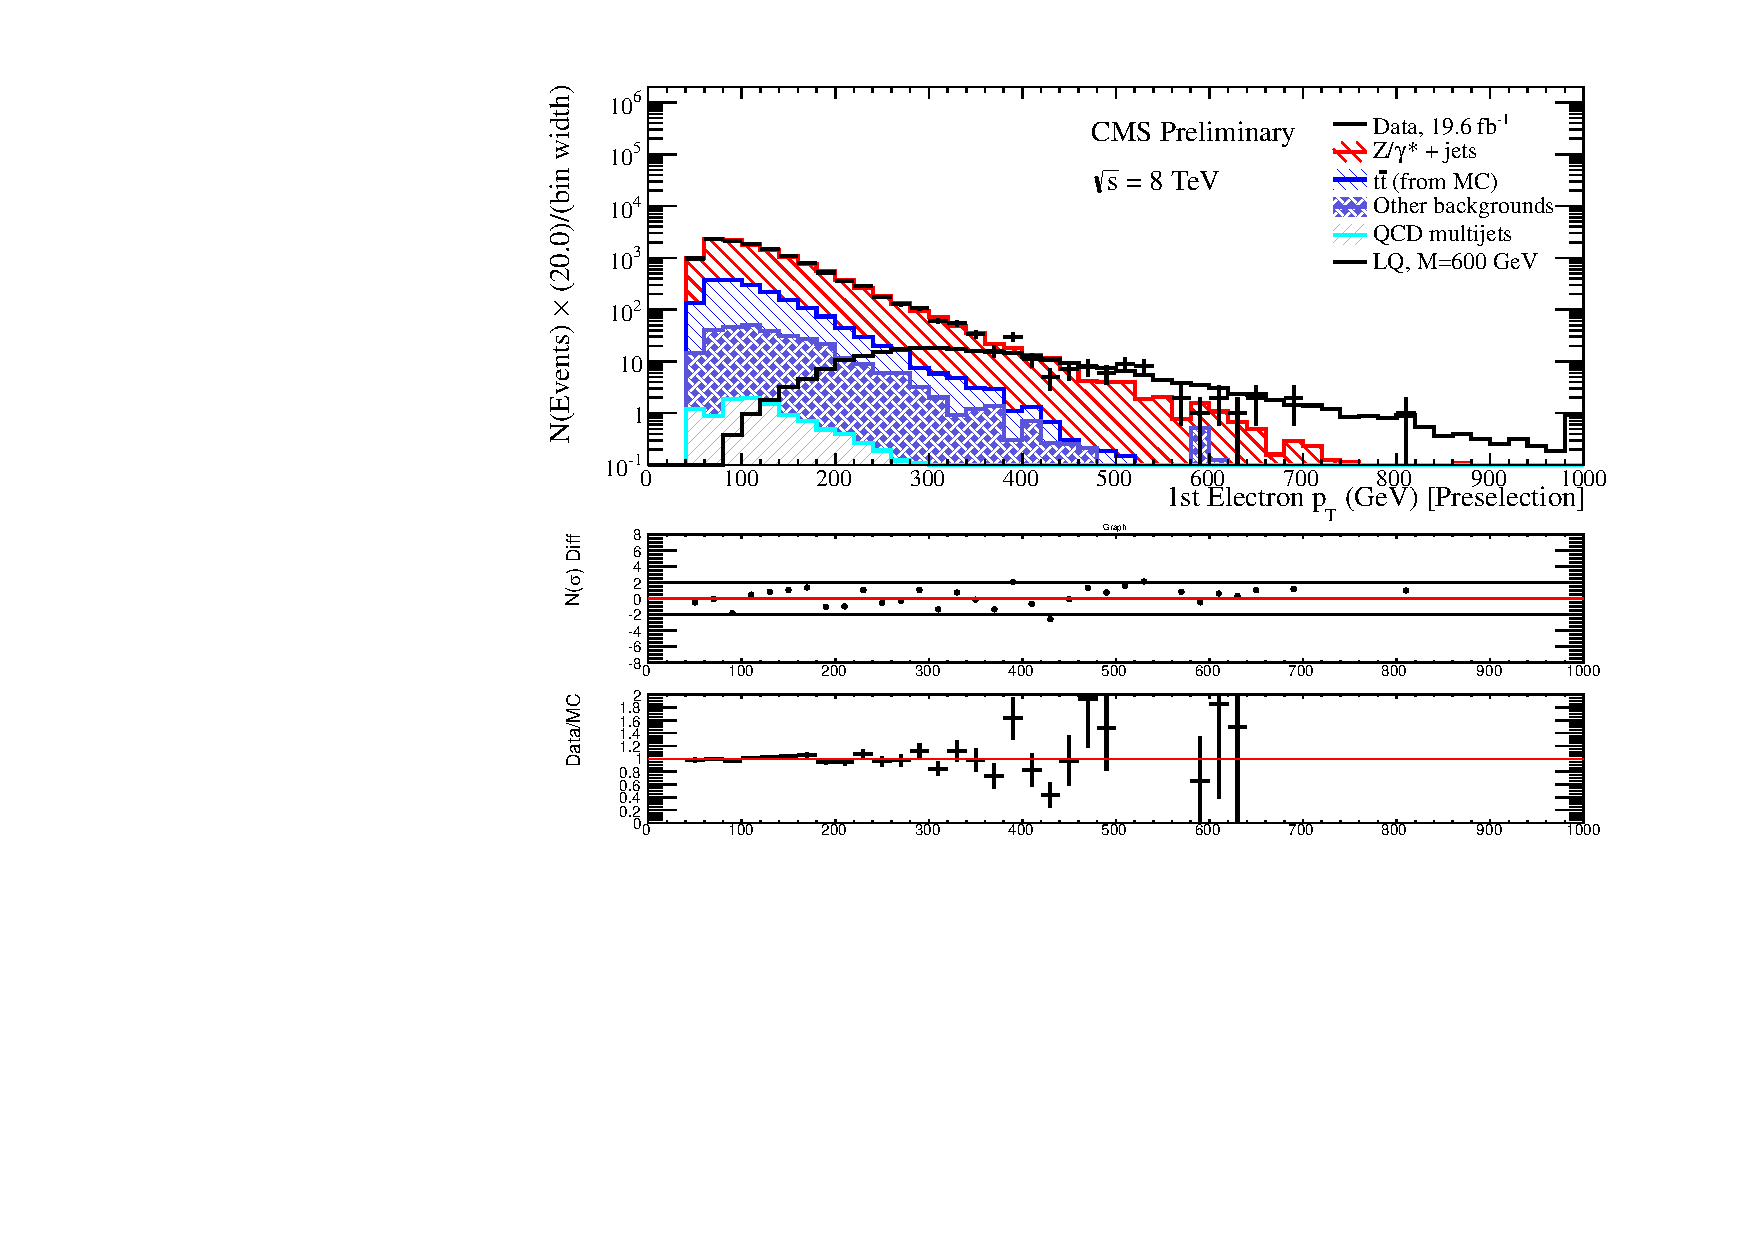
\includegraphics[width=\textwidth]{fig/ee/preselection/Pt1stEle_PAS_eejj.pdf}
\end{column}
\begin{column}{0.6\textwidth}
%% 2nd electron pt
\label{sec-1-1-1-2}

\centering
Second leading electron \pt
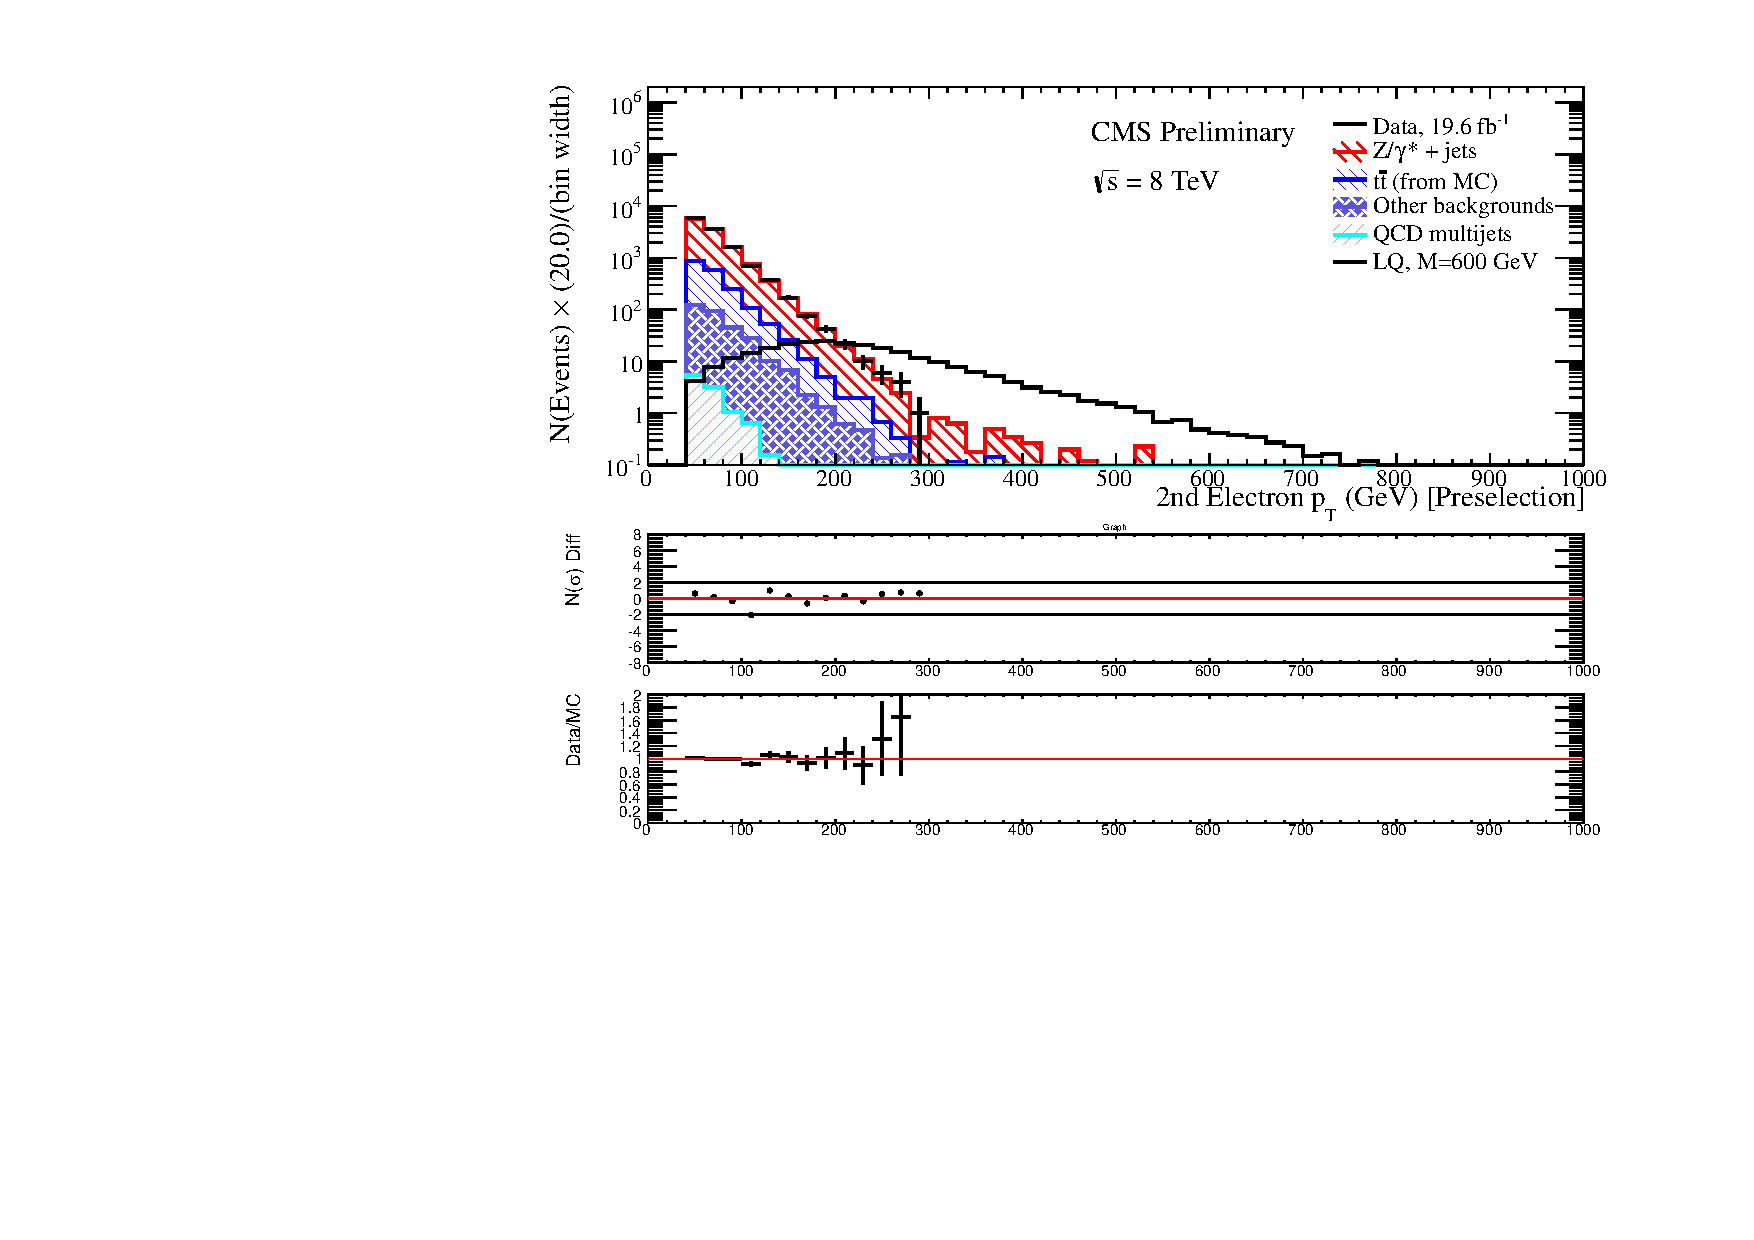
\includegraphics[width=\textwidth]{fig/ee/preselection/Pt2ndEle_PAS_eejj.pdf}
\end{column}
\end{columns}
\end{frame}
\begin{frame}
\frametitle{\eejj preselection: jet \pt}
\label{sec-1-1-2}
\begin{columns}
\begin{column}{0.6\textwidth}
%% 1st jet pt
\label{sec-1-1-2-1}

\centering
Leading jet \pt
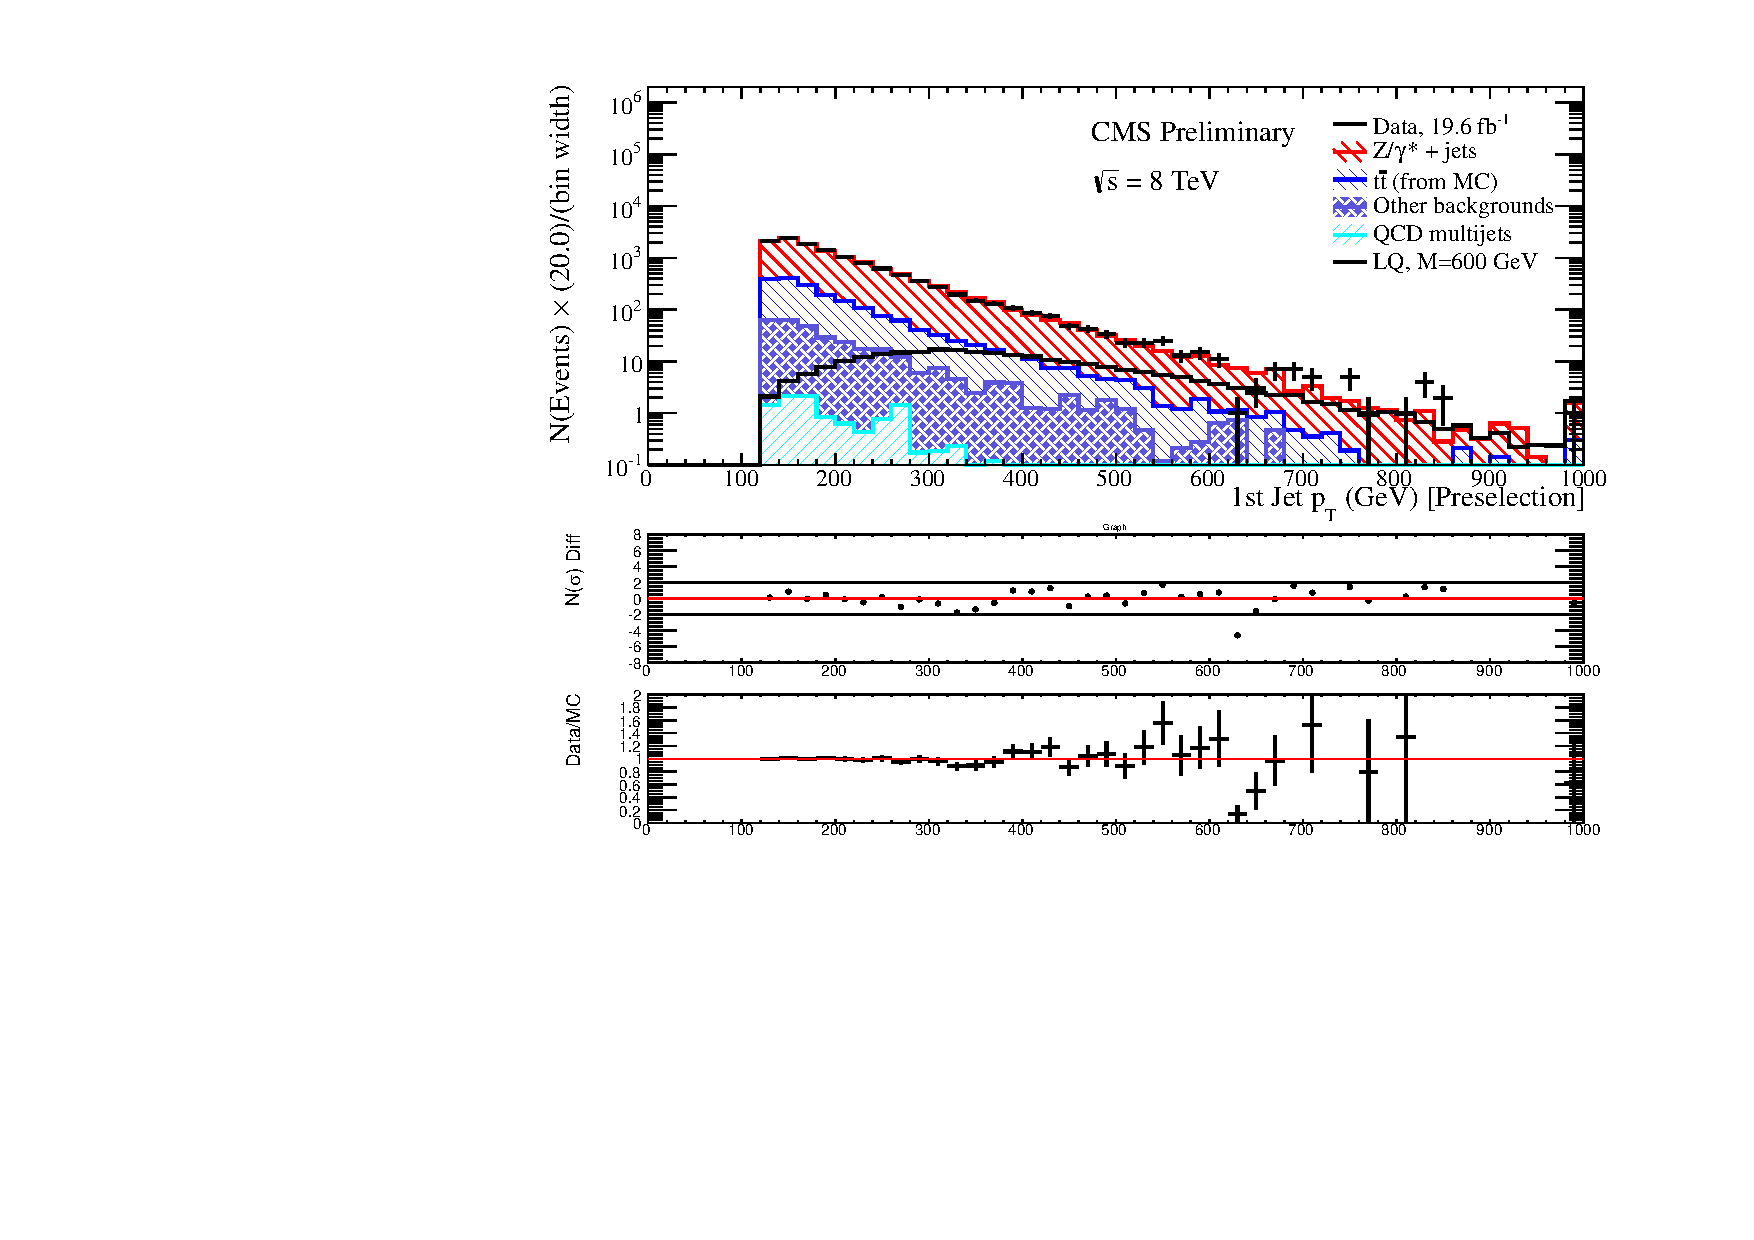
\includegraphics[width=\textwidth]{fig/ee/preselection/Pt1stJet_PAS_eejj.pdf}
\end{column}
\begin{column}{0.6\textwidth}
%% 2nd jet pt
\label{sec-1-1-2-2}

\centering
Second leading jet \pt
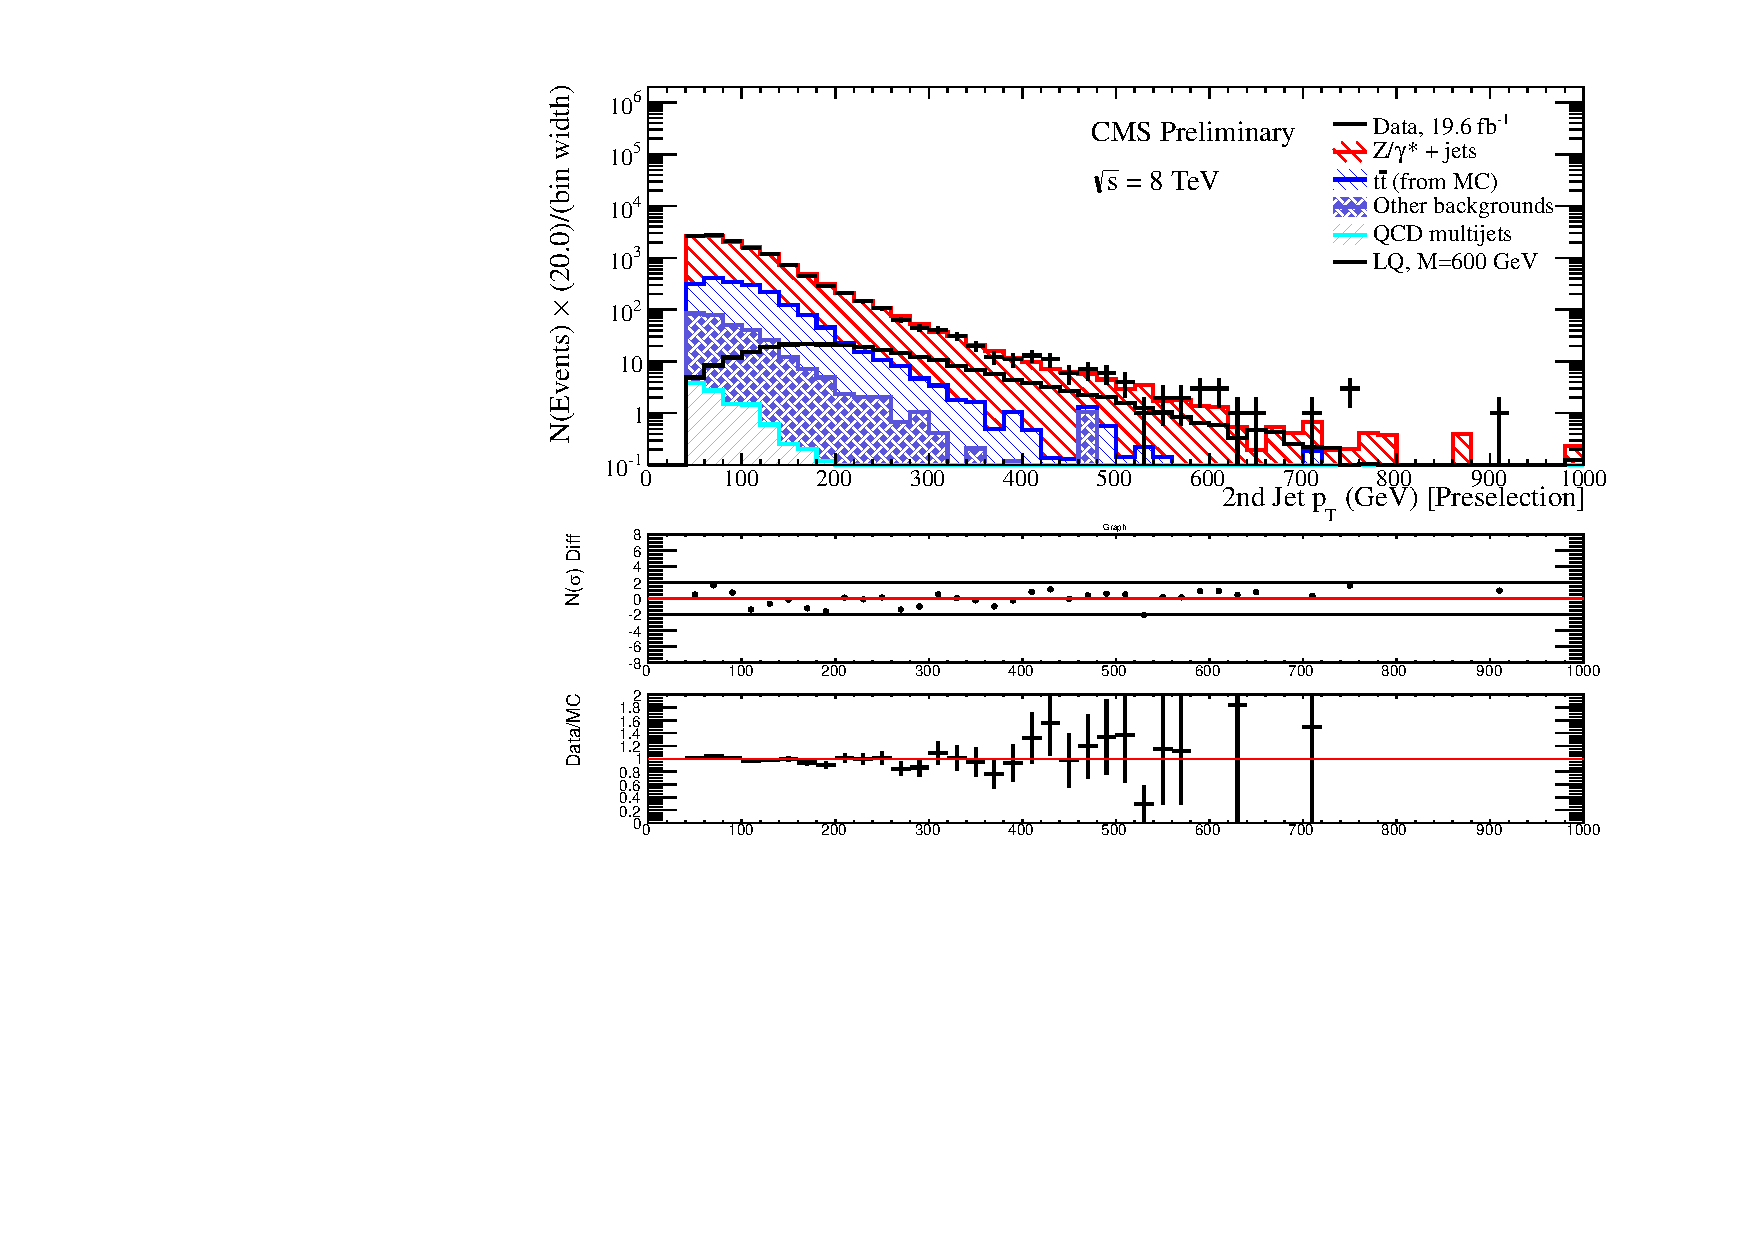
\includegraphics[width=\textwidth]{fig/ee/preselection/Pt2ndJet_PAS_eejj.pdf}
\end{column}
\end{columns}
\end{frame}
\subsection{\enujj preselection}
\label{sec-1-2}
\begin{frame}
\frametitle{\enujj preselection: electron \pt}
\label{sec-1-2-1}
\begin{columns}
\begin{column}{0.6\textwidth}
%% 1st electron pt
\label{sec-1-2-1-1}

\centering
Electron \pt
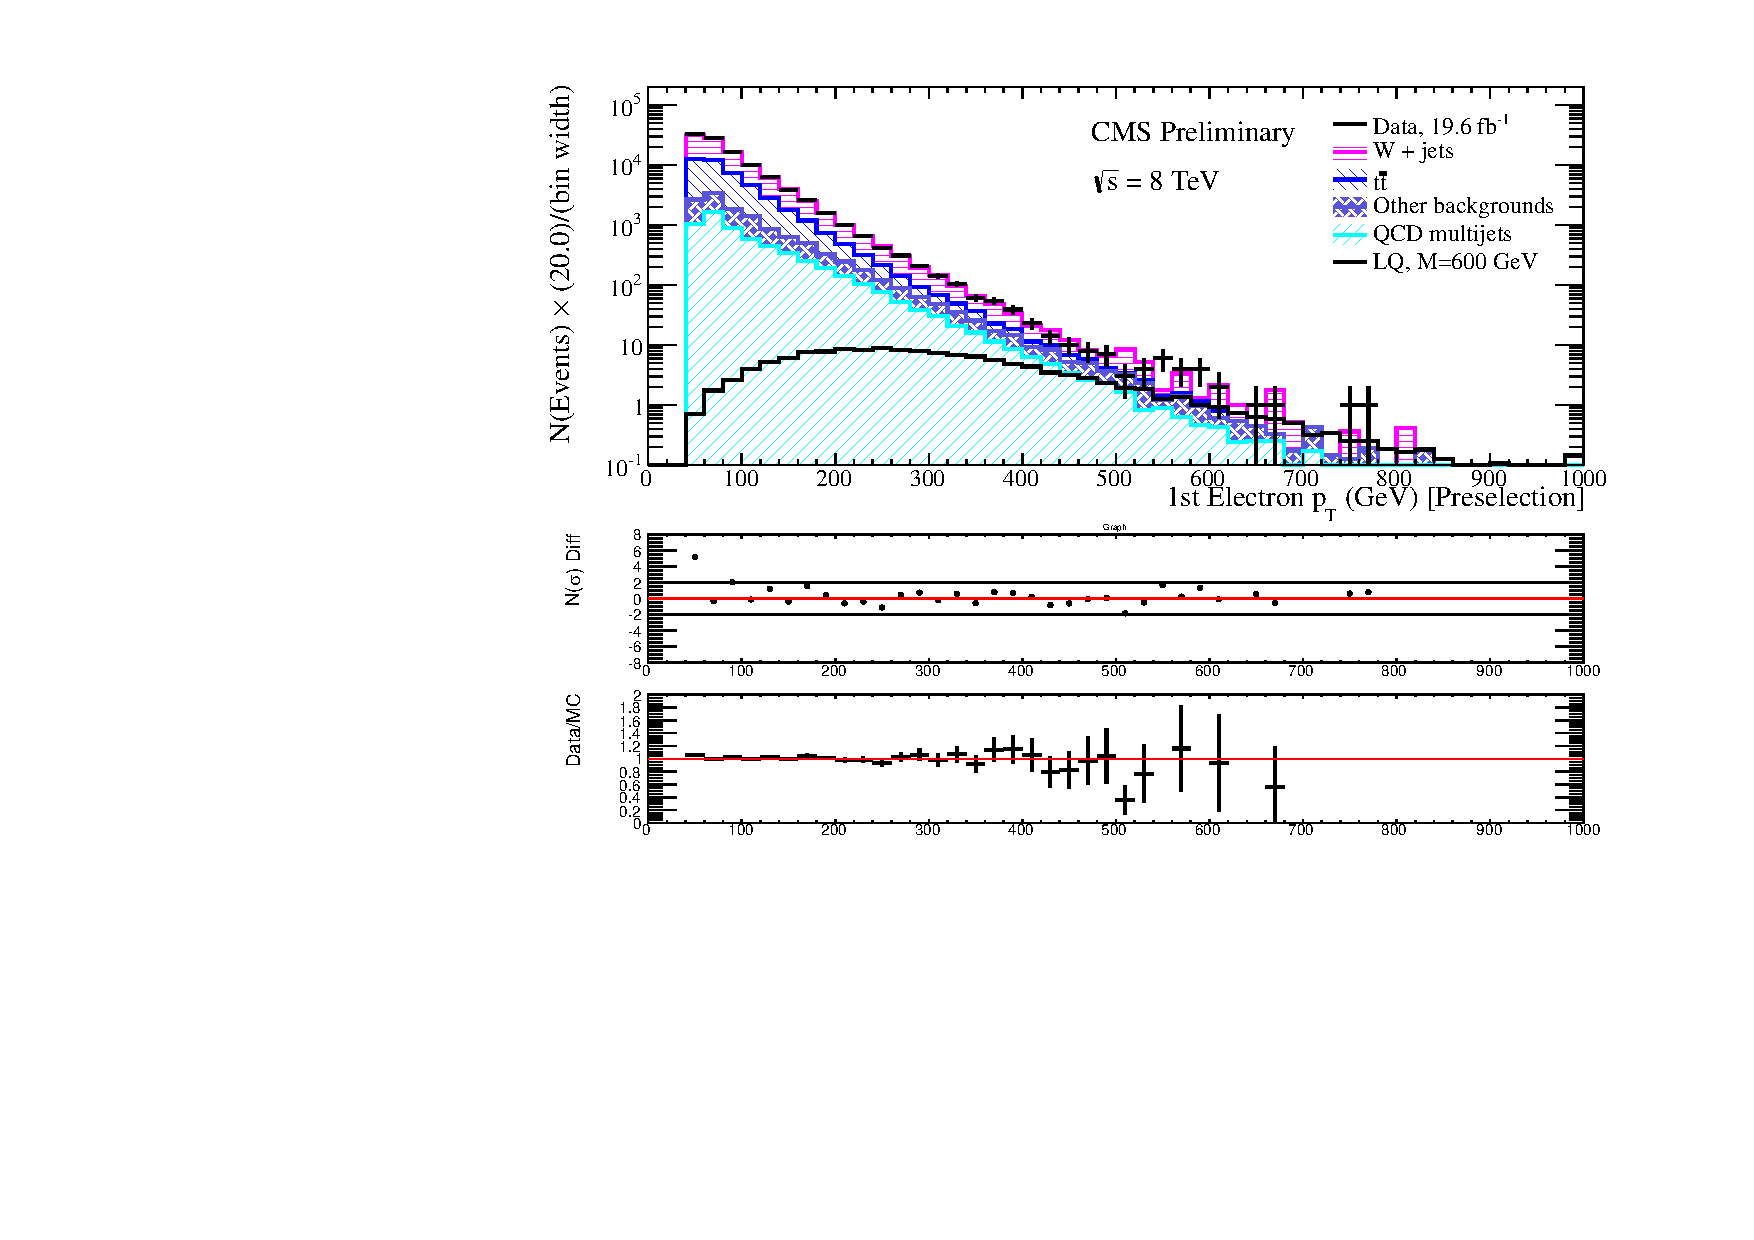
\includegraphics[width=\textwidth]{fig/enu/preselection/Pt1stEle_PAS_enujj.pdf}
\end{column}
\end{columns}
\end{frame}
\begin{frame}
\frametitle{\enujj preselection: jet \pt}
\label{sec-1-2-2}
\begin{columns}
\begin{column}{0.6\textwidth}
%% 1st jet pt
\label{sec-1-2-2-1}

\centering
Leading jet \pt
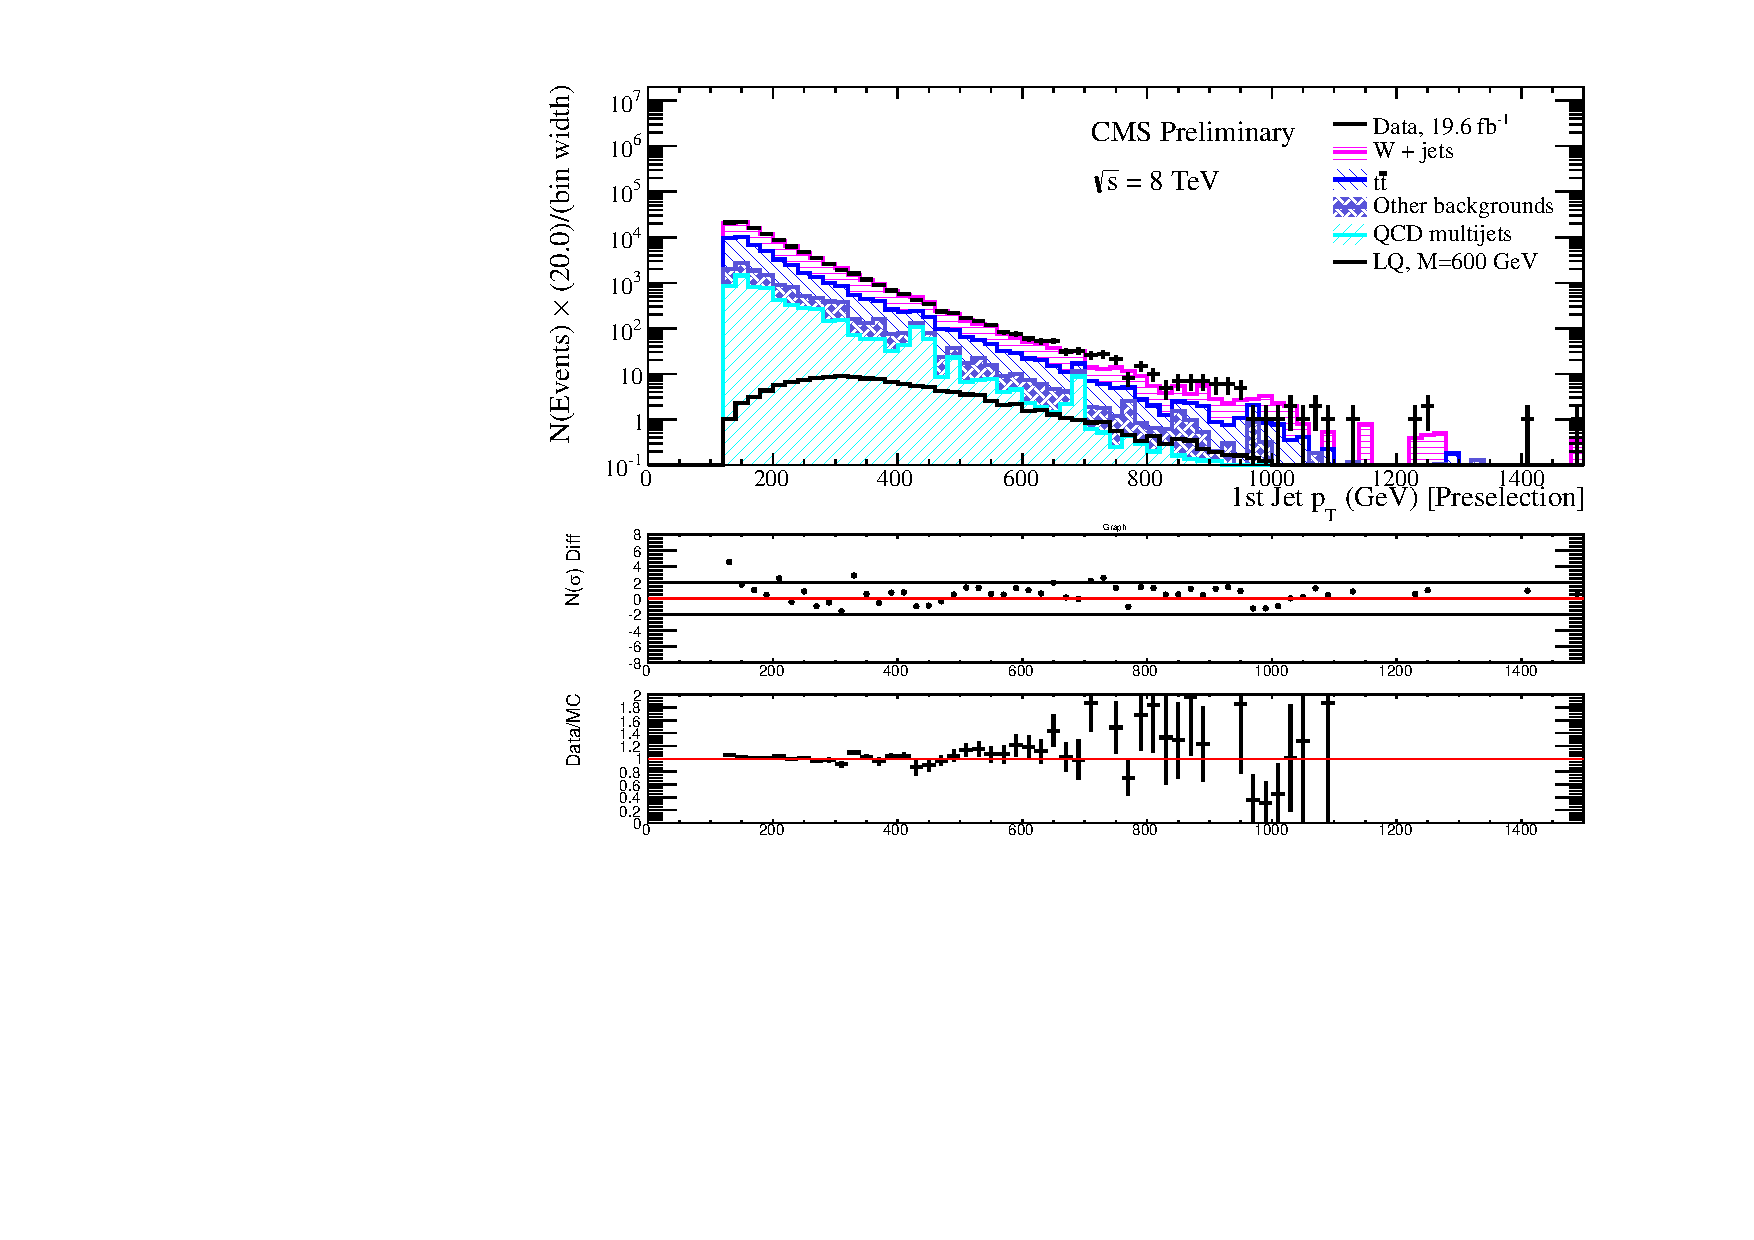
\includegraphics[width=\textwidth]{fig/enu/preselection/Pt1stJet_PAS_enujj.pdf}
\end{column}
\begin{column}{0.6\textwidth}
%% 2nd jet pt
\label{sec-1-2-2-2}

\centering
Second leading jet \pt
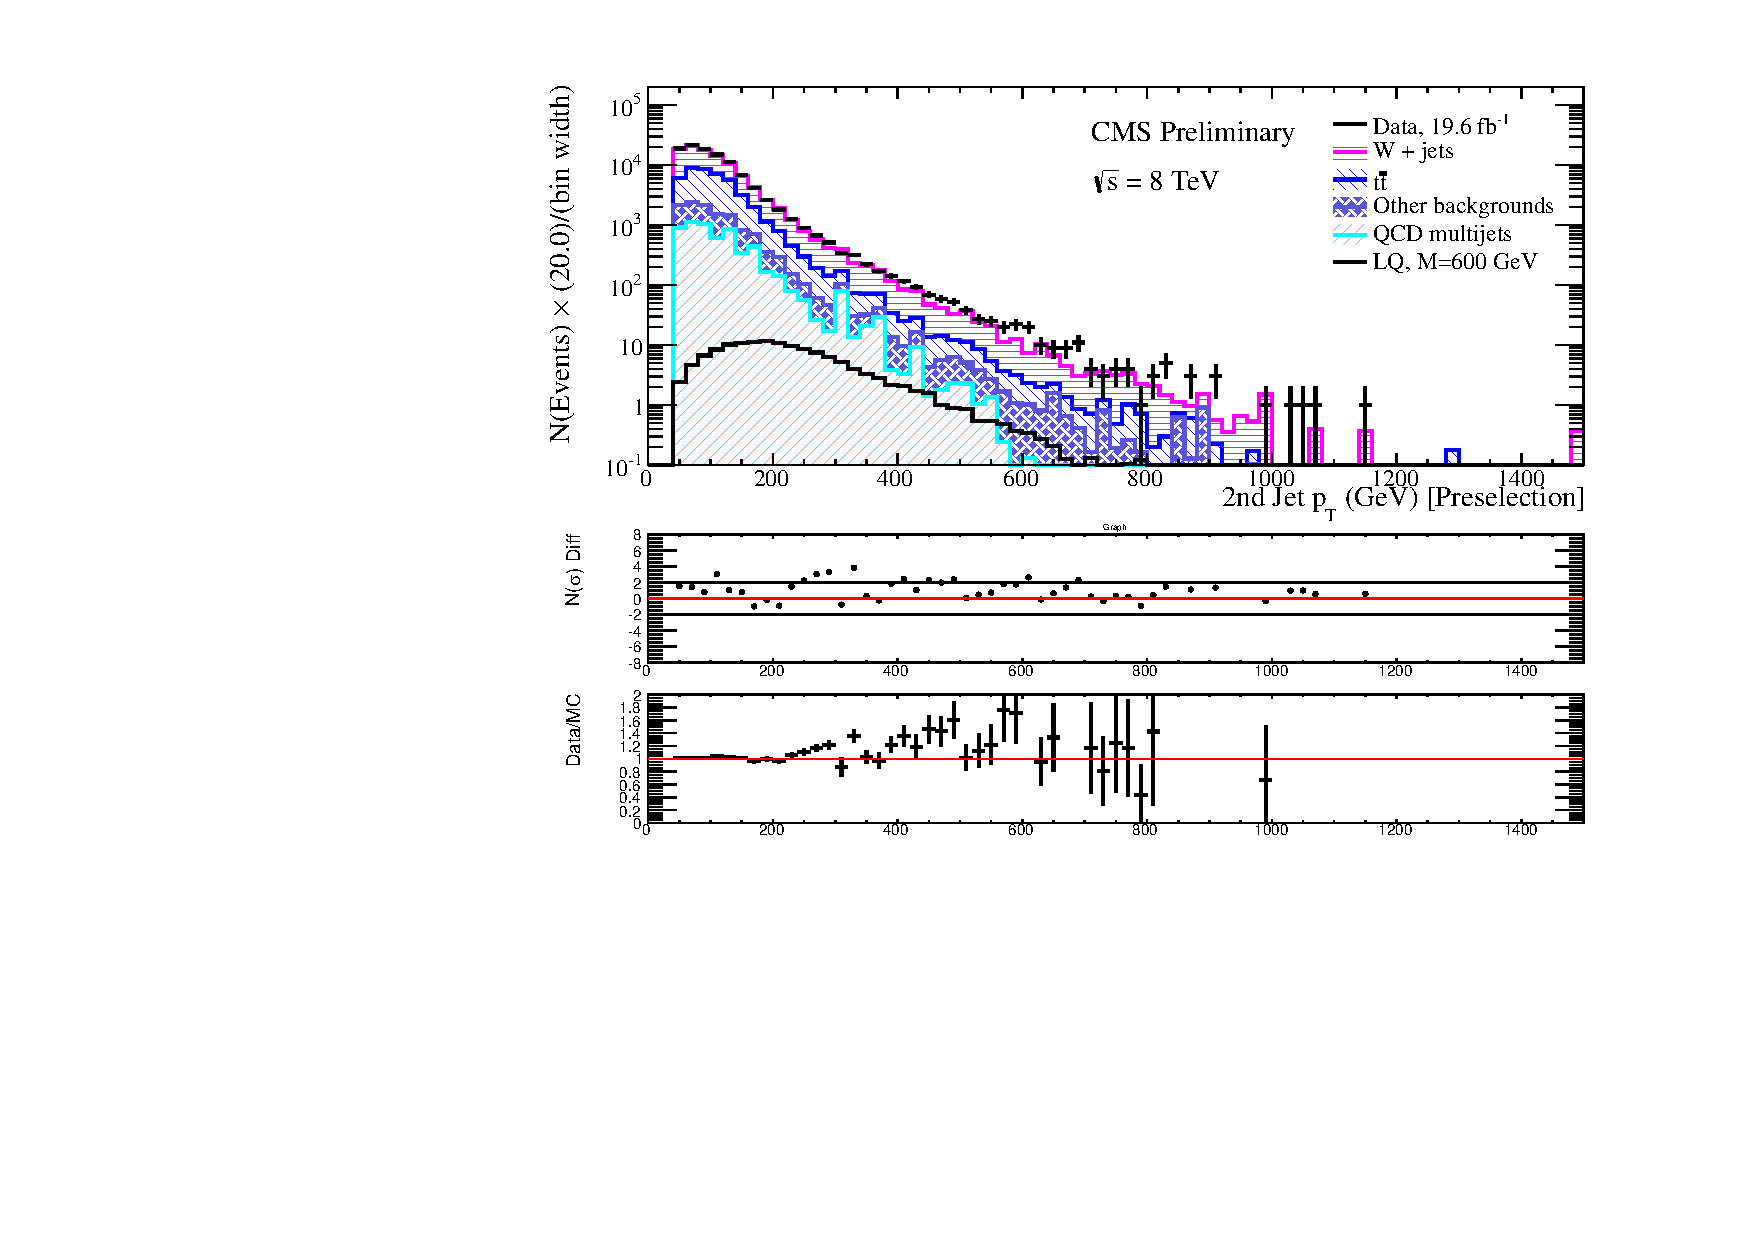
\includegraphics[width=\textwidth]{fig/enu/preselection/Pt2ndJet_PAS_enujj.pdf}
\end{column}
\end{columns}
\end{frame}
\subsection{\ttbar background in the \eejj analysis}
\label{sec-1-3}
\begin{frame}
\frametitle{\ttbar background in \eejj analysis: weights}
\label{sec-1-3-1}

\centering
\begin{tabular}{|c|c|}
\hline
\hline
Muon $|\eta|$ range & Weight applied to \emujj~events \\
\hline
\hline
$0.0 < |\eta| \leq 0.9$ & $\mathcal{C} = 0.458  \pm 0.005$ (stat) $\pm 0.005$ (syst)\\
$0.9 < |\eta| \leq 1.2$ & $\mathcal{C} = 0.409  \pm 0.005$ (stat) $\pm 0.005$ (syst)\\
$1.2 < |\eta| \leq 2.1$ & $\mathcal{C} = 0.400  \pm 0.005$ (stat) $\pm 0.005$ (syst)\\
\hline
\hline
\end{tabular}
\end{frame}
\begin{frame}
\frametitle{\ttbar background in \eejj analysis: triggers}
\label{sec-1-3-2}

\centering
\begin{tabular}{|l|c|}
\hline
\hline
HLT path & Run range \\
\hline
\hline
{\tt HLT\_Mu40\_eta2p1\_v9}  & 190456 - 196531 \\
{\tt HLT\_Mu40\_eta2p1\_v10} & 198063 - 199608 \\
{\tt HLT\_Mu40\_eta2p1\_v11} & 199698 - 208686 \\
\hline
\hline
\end{tabular}
\end{frame}
\subsection{QCD background in both analyses}
\label{sec-1-4}
\begin{frame}
\frametitle{QCD background: triggers}
\label{sec-1-4-1}
%% Trigger table
\label{sec-1-4-1-1}

\centering
\resizebox*{!}{0.8\textheight}{
\begin{tabular}{|l|c|c|}
\hline
\hline
HLT path & Run range & Effective $\mathcal{L}_{int}(\text{pb}^{-1})$ \\
\hline
\hline
{\tt HLT\_Photon30\_CaloIdVL\_v11} & 190456 - 190738 & 0.029672 \\
{\tt HLT\_Photon30\_CaloIdVL\_v12} & 190782 - 191419 & 0.086121 \\
{\tt HLT\_Photon30\_CaloIdVL\_v13} & 191691 - 196531 & 0.690924 \\
{\tt HLT\_Photon30\_CaloIdVL\_v14} & 198022 - 208686 & 2.043    \\
\hline
{\tt HLT\_Photon50\_CaloIdVL\_v7}  & 190456 - 190738 & 0.231664 \\
{\tt HLT\_Photon50\_CaloIdVL\_v8}  & 190782 - 191419 & 0.669828 \\
{\tt HLT\_Photon50\_CaloIdVL\_v9}  & 191691 - 196531 & 5.374    \\
{\tt HLT\_Photon50\_CaloIdVL\_v10} & 198022 - 208686 & 15.894   \\
\hline
{\tt HLT\_Photon75\_CaloIdVL\_v10} & 190456 - 190738 & 1.385    \\
{\tt HLT\_Photon75\_CaloIdVL\_v11} & 190782 - 191419 & 4.019    \\
{\tt HLT\_Photon75\_CaloIdVL\_v12} & 191691 - 196531 & 32.243   \\
{\tt HLT\_Photon75\_CaloIdVL\_v13} & 198022 - 208686 & 95.363   \\
\hline
{\tt HLT\_Photon90\_CaloIdVL\_v7}  & 190456 - 190738 & 2.769    \\
{\tt HLT\_Photon90\_CaloIdVL\_v8}  & 190782 - 191419 & 8.038    \\
{\tt HLT\_Photon90\_CaloIdVL\_v9}  & 191691 - 196531 & 69.509   \\
{\tt HLT\_Photon90\_CaloIdVL\_v10} & 198022 - 208686 & 198.024  \\
\hline
{\tt HLT\_Photon135\_v4}               & 190456 - 190738 & 96.404   \\
{\tt HLT\_Photon135\_v5}               & 190782 - 191419 & 398.151  \\
{\tt HLT\_Photon135\_v6}               & 191691 - 196531 & 543.603  \\
{\tt HLT\_Photon135\_v7}               & 198022 - 208686 & 12581    \\
\hline
{\tt HLT\_Photon150\_v1}               & 190456 - 190738 & 96.404   \\
{\tt HLT\_Photon150\_v2}               & 190782 - 191419 & 398.151  \\
{\tt HLT\_Photon150\_v3}               & 191691 - 196531 & 4824.    \\
{\tt HLT\_Photon150\_v4}               & 198022 - 208686 & 14304    \\
\hline
\hline
\end{tabular}
}
\end{frame}
\begin{frame}
\frametitle{QCD background: closure test method (1/2)}
\label{sec-1-4-2}
%% Text
\label{sec-1-4-2-1}

\small
\begin{itemize}
\item Define closure test sample:
\begin{itemize}
\small
\item Single photon trigger (same as calculation)
\item Exactly two loose electrons
\item At least one jet
\item $\mee > 110$ GeV, to improve QCD purity
\item $\met < 100$ GeV, to improve QCD purity
\end{itemize}
\item Subtract contribution from non-QCD processes using MC
\item Predict N(events) with exactly one HEEP electron and at least one jet with fake rate:
\end{itemize}
\begin{align*}
N_{eejj}^{QCD}  &= \sum_{\substack{\text{loose} \\\eejj \text{ events}}} P(e_{\text{1, tight}} | e_{\text{1, loose}}:\pt, \eta) \cdot P(e_{\text{2, tight}} | e_{\text{2, loose}}:\pt, \eta) \\
\end{align*}
\end{frame}
\begin{frame}
\frametitle{QCD background: closure test method (2/2)}
\label{sec-1-4-3}
%% Text
\label{sec-1-4-3-1}

\scriptsize
\begin{itemize}
\item Finally, compare predicted vs observed N(events) with exactly one HEEP electron:
\begin{itemize}
\scriptsize
\item N(predicted) = $13100 \pm 400$
\item N(observed)  = $12100 \pm 400$
\item N(predicted)/N(observed) = $1.08 \pm 0.05$
\end{itemize}

\item After applying $\ST = \pt(e_1) + \pt(e_2) + \pt(j) > 450$ GeV \\
(comparable to final selection \ST cut), agreement worsens:
\begin{itemize}
\scriptsize
\item N(predicted) = $599 \pm 53.6$
\item N(observed)  = $876 \pm 46.7$
\item N(predicted)/N(observed) = $1.46 \pm 0.15$
\end{itemize}

\item Best agreement given $1\sigma$ fluctuation at $\ST > 450$ is 30\%,
so we assign a systematic uncertainty of 30\% per electron to the QCD
background estimate.
\end{itemize}
\end{frame}
\begin{frame}
\frametitle{QCD background: closure test plots}
\label{sec-1-4-4}
\begin{columns}
\begin{column}{0.6\textwidth}
%% First electron pt
\label{sec-1-4-4-1}

\centering
Leading electron \pt
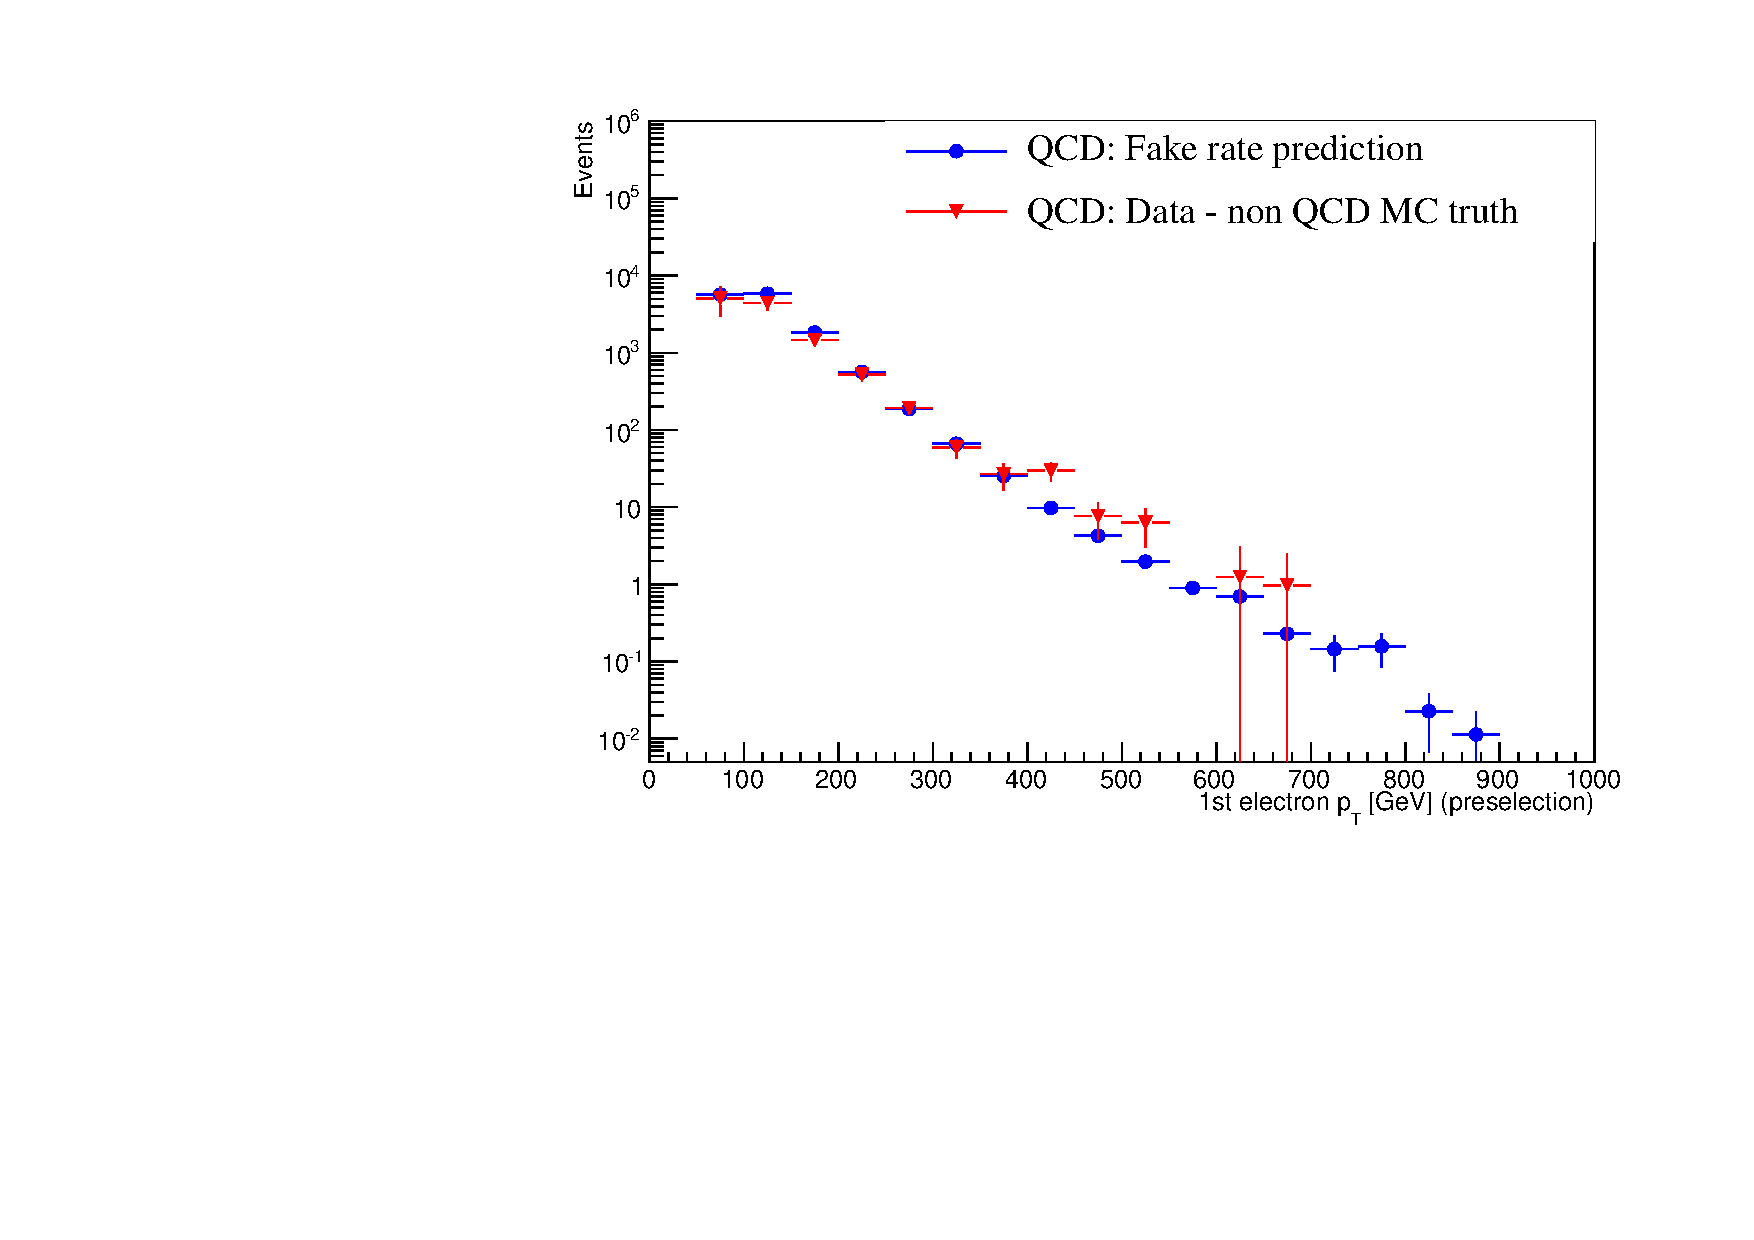
\includegraphics[width=\textwidth]{fig/qcd/closure_test/Pt1stEle_PAS.pdf}
\end{column}
\begin{column}{0.6\textwidth}
%% ST
\label{sec-1-4-4-2}

\centering
\ST
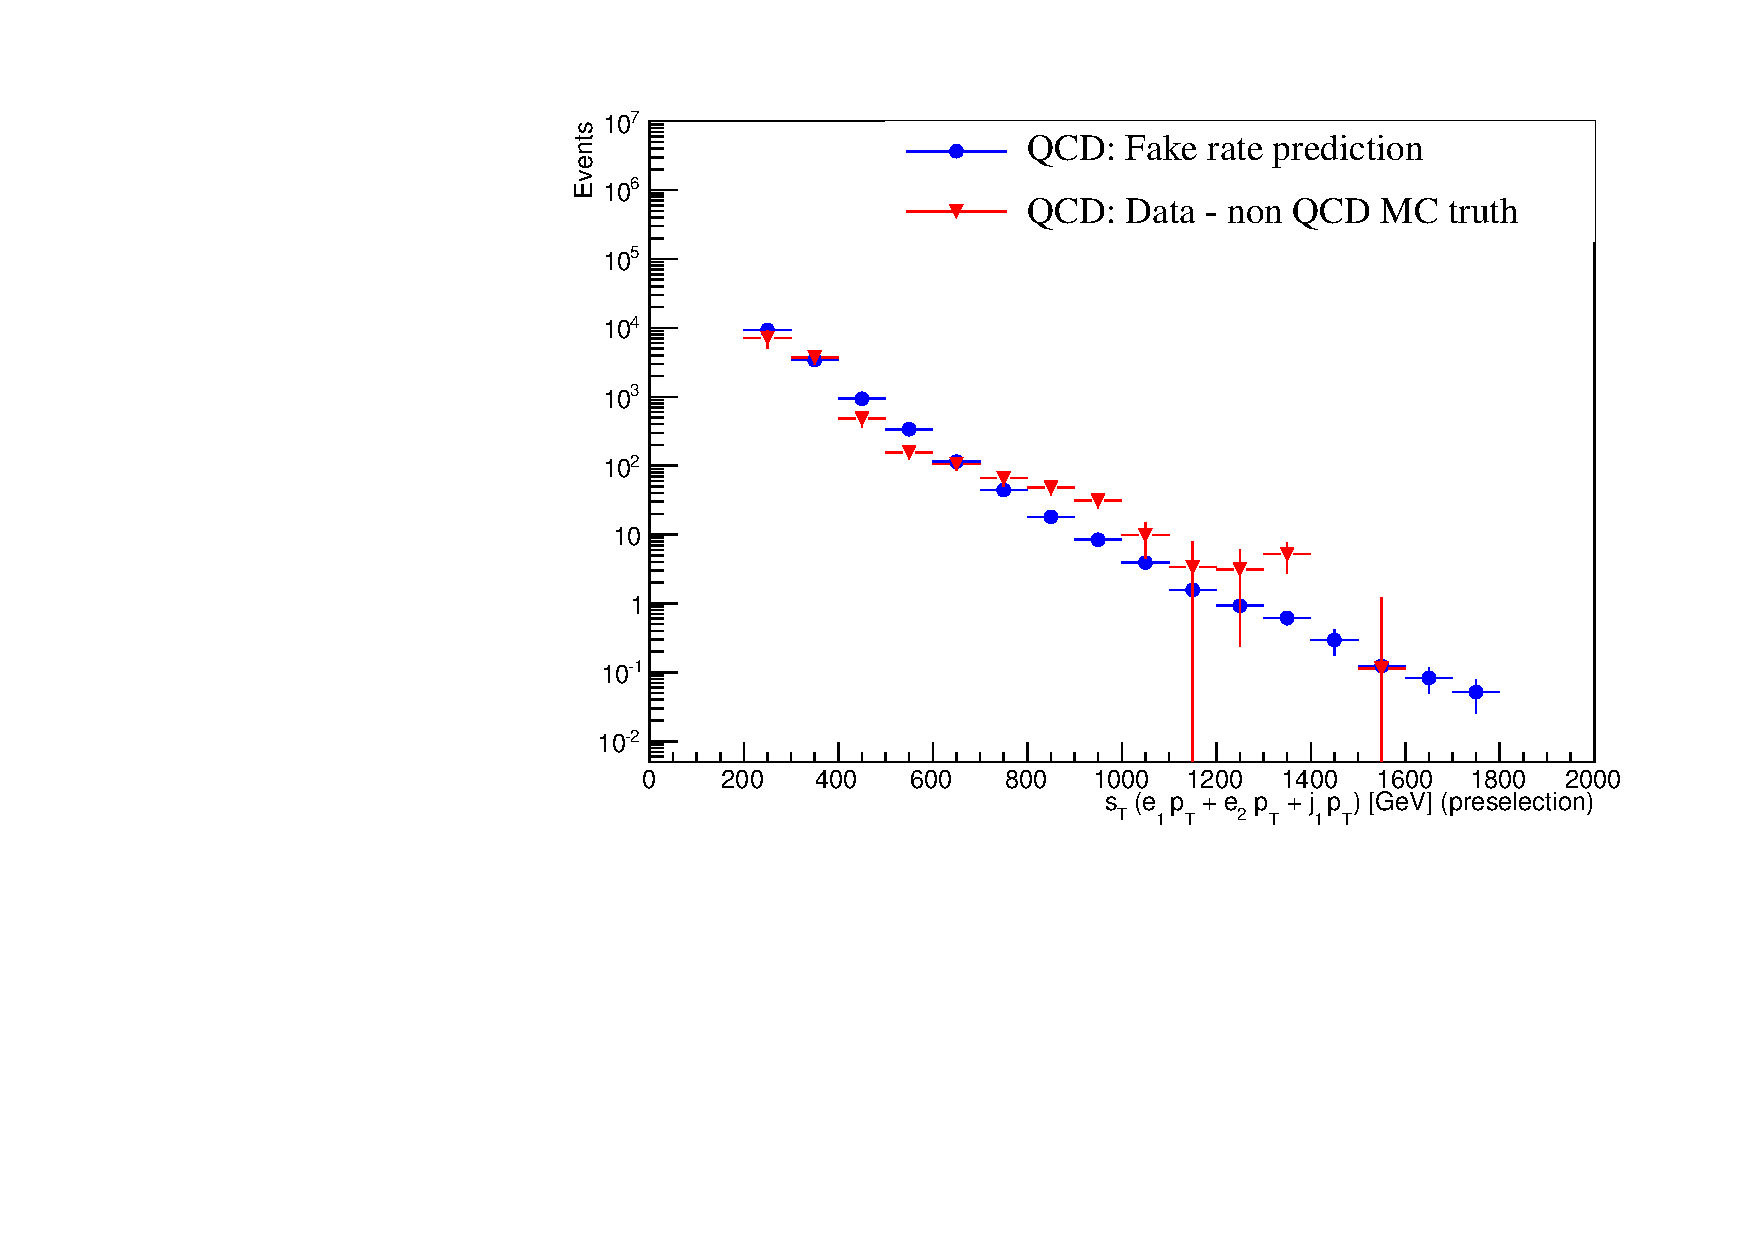
\includegraphics[width=\textwidth]{fig/qcd/closure_test/sT_PAS.pdf}
\end{column}
\end{columns}
\end{frame}
\subsection{Run period dependence}
\label{sec-1-5}
\begin{frame}
\frametitle{Run period dependence}
\label{sec-1-5-1}
\begin{columns} % Columns
\label{sec-1-5-1-1}
\begin{column}{0.5\textwidth}
%% eejj
\label{sec-1-5-1-1-1}

\centering
Events passing \eejj \\
$M_{LQ} = 650$ GeV selection
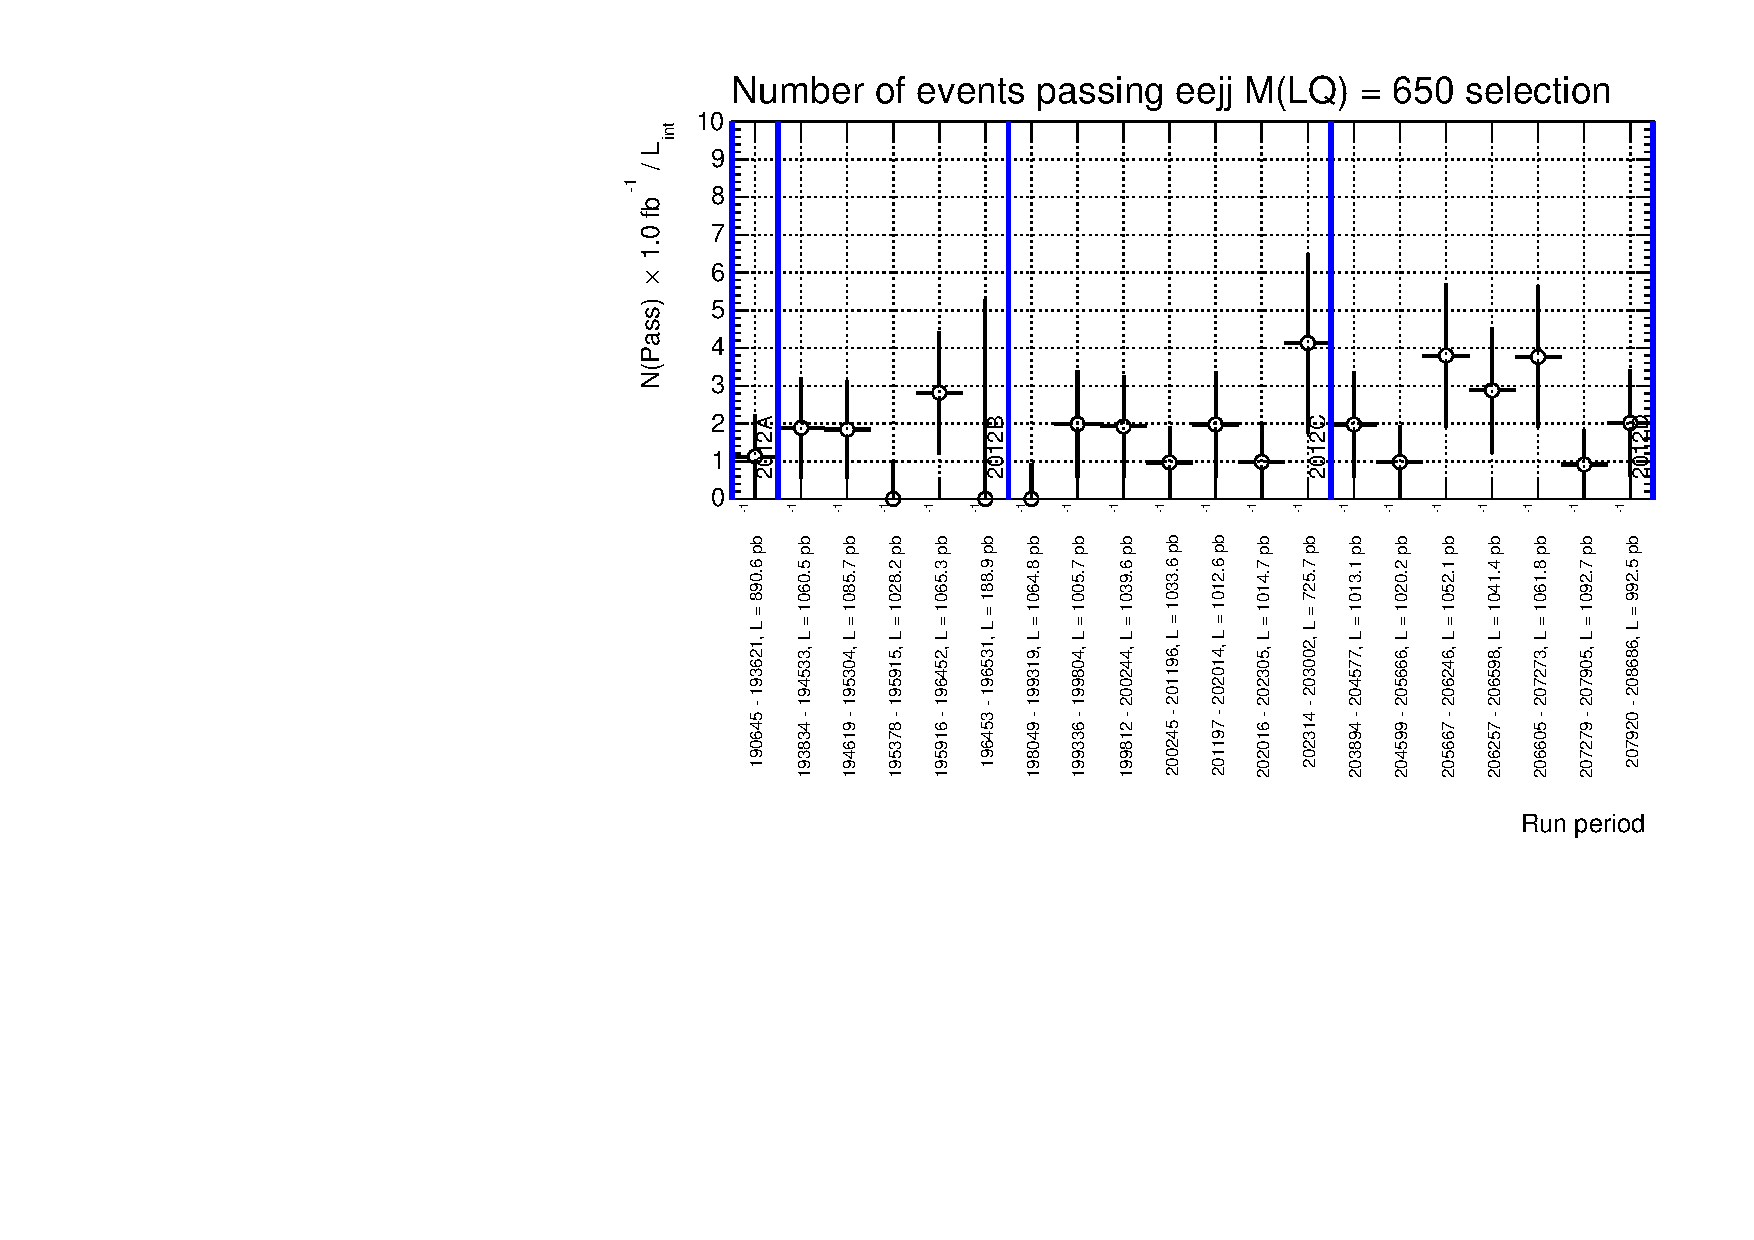
\includegraphics[width=\textwidth]{fig/ee/run_dependence/nEventsPassing_eejj_LQM650.pdf}
\end{column}
\begin{column}{0.5\textwidth}
%% enujj
\label{sec-1-5-1-1-2}

\centering
Events passing \enujj \\
$M_{LQ} = 650$ GeV selection
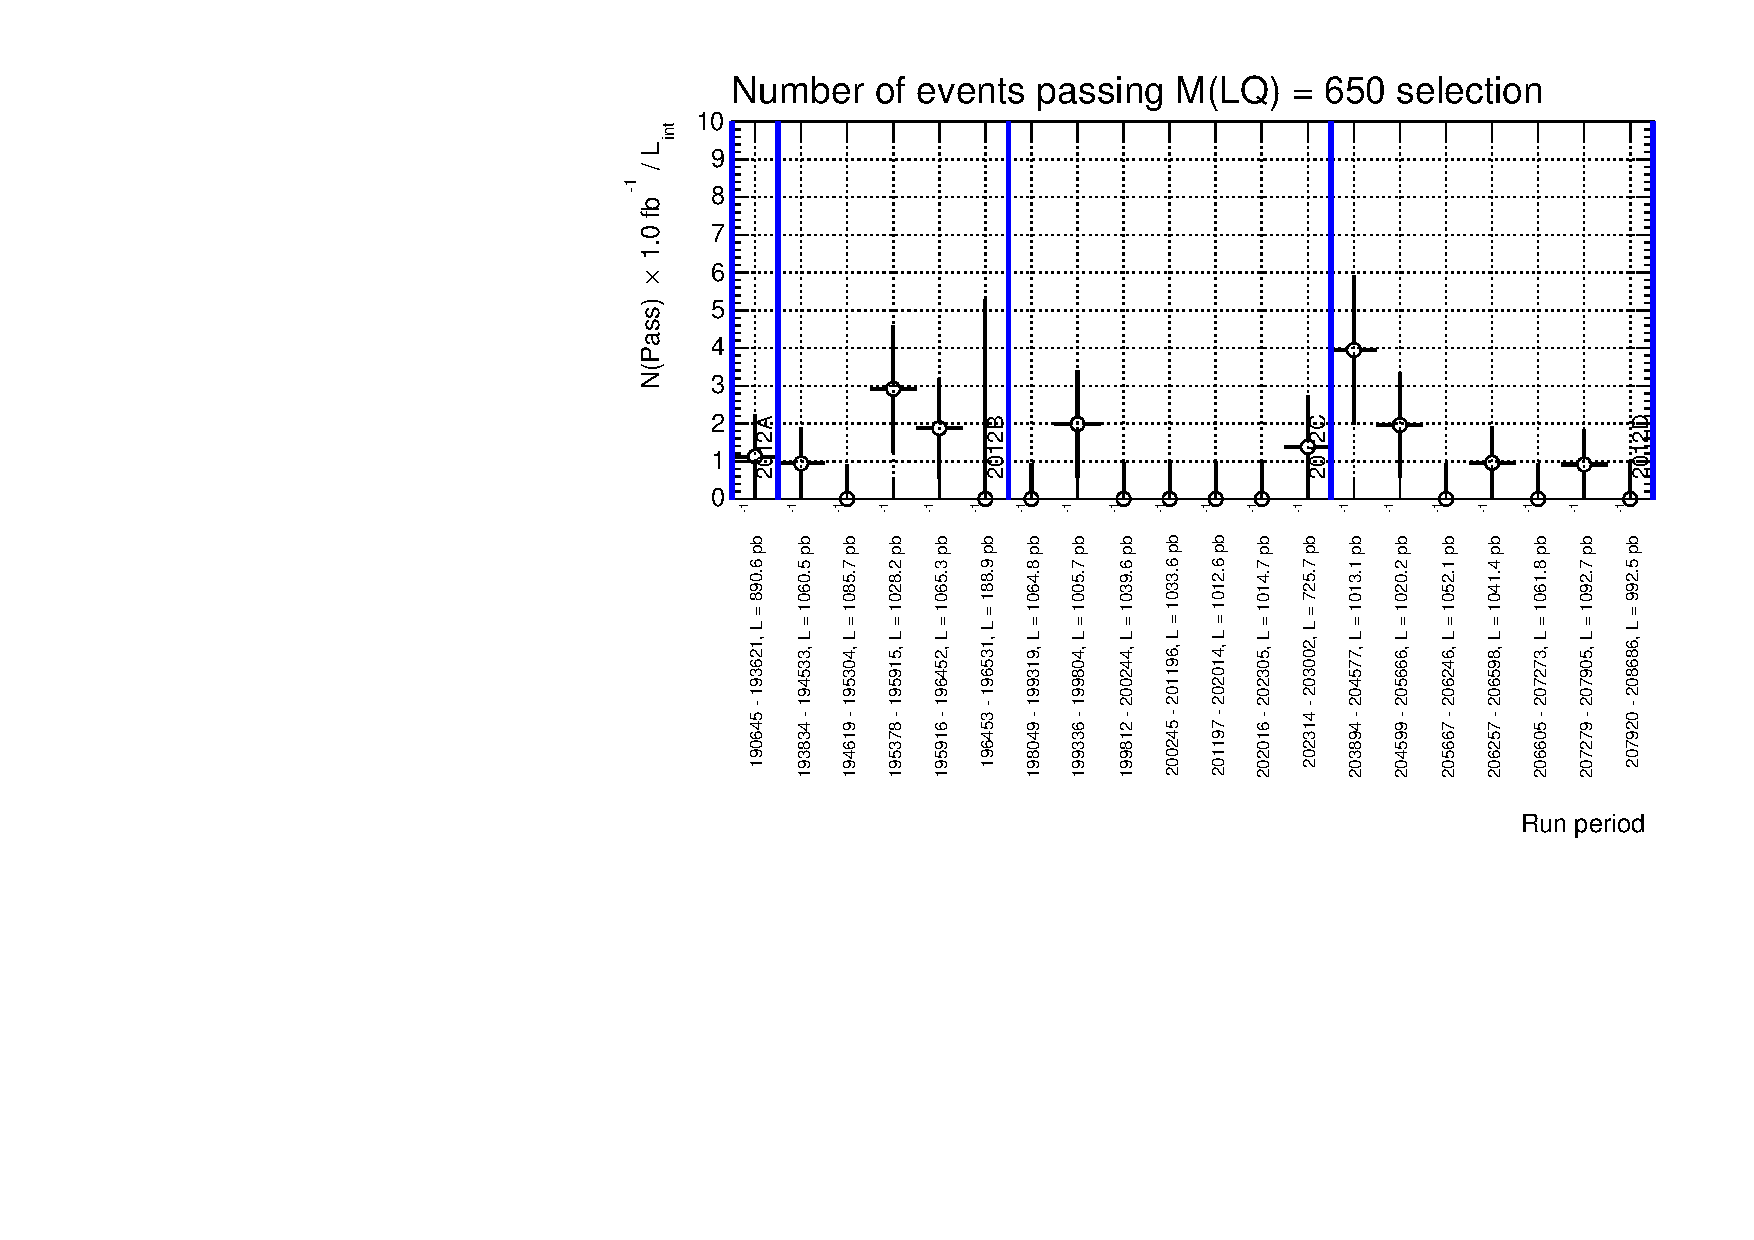
\includegraphics[width=\textwidth]{fig/enu/run_dependence/nEventsPassing_enujj_LQM650.pdf}
\end{column}
\end{columns}
%% Note
\label{sec-1-5-1-2}

\small
\centering
Events passing final selection in both analyses are evenly distributed in time
\normalsize
\end{frame}
\subsection{Data-driven background using muons}
\label{sec-1-6}
\begin{frame}
\frametitle{Data-driven background using muons: overview}
\label{sec-1-6-1}
%% Text
\label{sec-1-6-1-1}

\begin{itemize}
\item Use muon events to simulate electron events:
\begin{itemize}
\item \eejj analysis: use \mumujj events
\begin{equation*}
  N_{\eejj}^{\text{data}} = \mathcal{C}_{\mumujj} \times N_{\mumujj}^{\text{data}} = \left( \frac{\epsilon^{\text{trigger}}_{ejj}}{\epsilon^{\text{trigger}}_{\mu}} \times \frac{\epsilon^{\text{reco} / \text{ID} / \text{Iso}}_{\eejj}}{\epsilon^{\text{reco} / \text{ID} / \text{Iso}}_{\mumujj}} \right) \times N_{\mumujj}^{\text{data}}
\end{equation*}
\item \enujj analysis: use \munujj events
\begin{equation*}
  N_{\enujj}^{\text{data}} = \mathcal{C}_{\munujj} \times N_{\munujj}^{\text{data}} = \left( \frac{\epsilon^{\text{trigger}}_{ejj}}{\epsilon^{\text{trigger}}_{\mu}} \times \frac{\epsilon^{\text{reco} / \text{ID} / \text{Iso}}_{\enujj}}{\epsilon^{\text{reco} / \text{ID} / \text{Iso}}_{\munujj}} \right) \times N_{\munujj}^{\text{data}}
\end{equation*}
\end{itemize}
\item Still use QCD fake rate method to model "fake" electrons
\item \alert{Only used as a cross-check!}
\end{itemize}
\end{frame}
\begin{frame}
\frametitle{Data-driven background using muons: \eejj (1/2)}
\label{sec-1-6-2}
\begin{columns} % Plots
\label{sec-1-6-2-1}
\begin{column}{0.6\textwidth}
%% M(ee)
\label{sec-1-6-2-1-1}

\centering
\mee at \eejj preselection
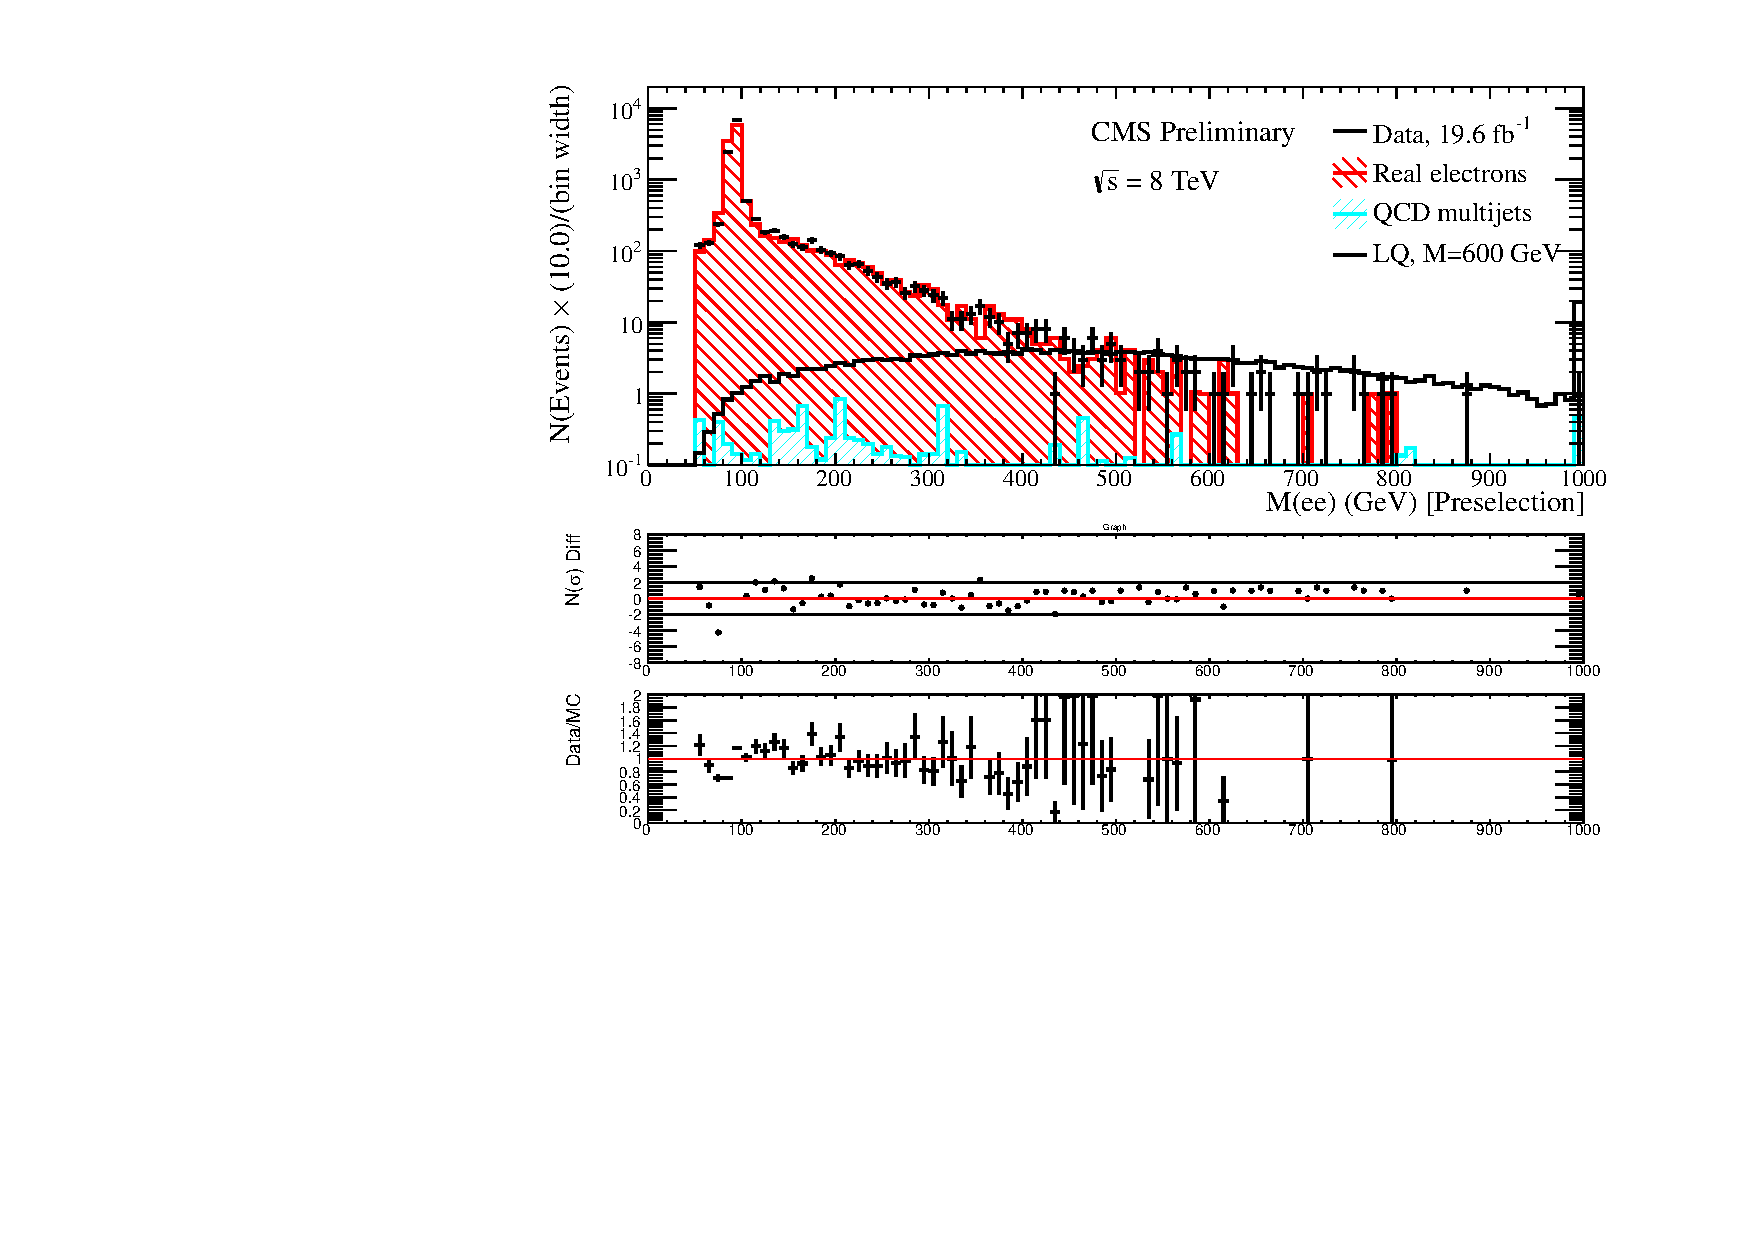
\includegraphics[width=0.875\textwidth]{fig/ee/muonbackground/Mee_PAS_eejj.pdf}
\end{column}
\begin{column}{0.6\textwidth}
%% ST
\label{sec-1-6-2-1-2}

\centering
\ST at \eejj preselection
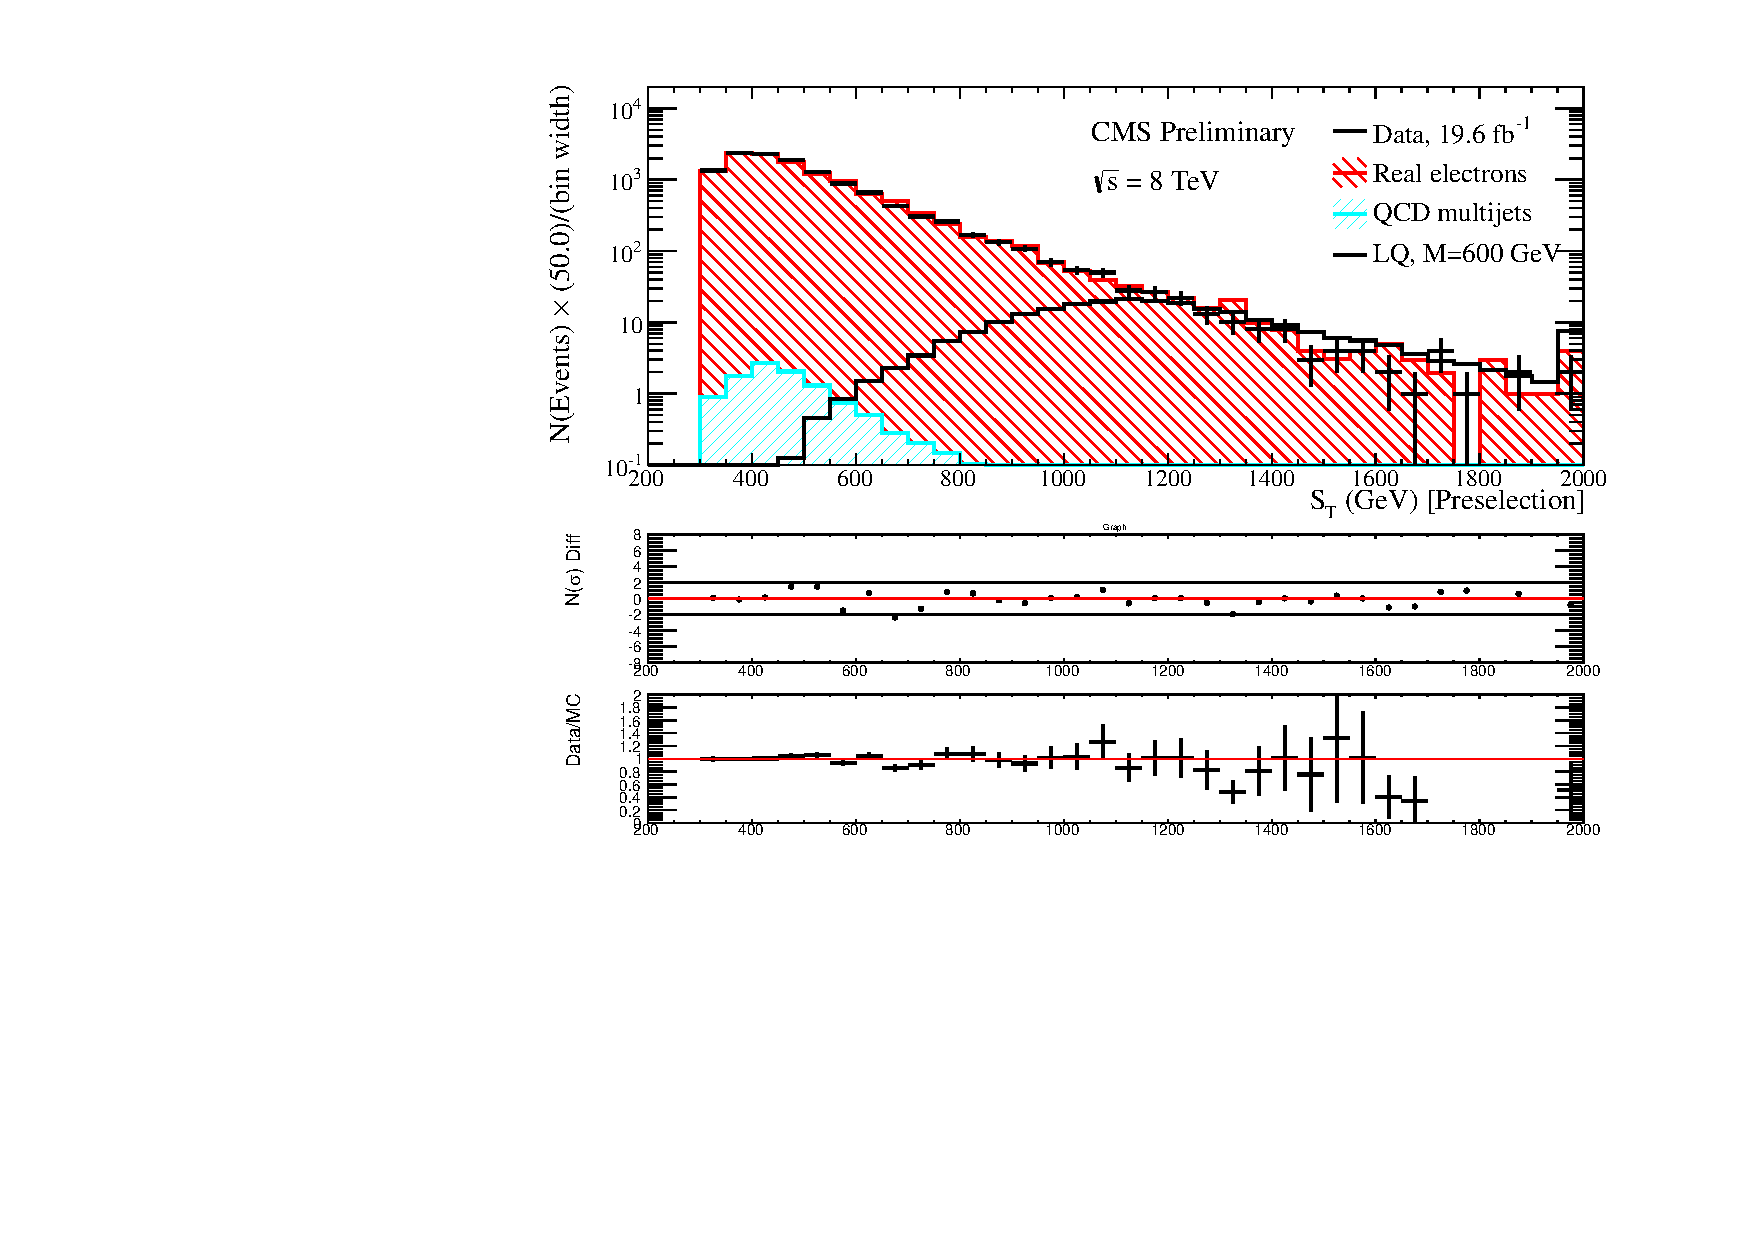
\includegraphics[width=0.875\textwidth]{fig/ee/muonbackground/sT_PAS_eejj.pdf}
\end{column}
\end{columns}
%% Text
\label{sec-1-6-2-2}

\footnotesize
\begin{itemize}
\item "Real electrons": \eejj events with no fake electrons \\
(modeled with \mumujj)
\item Difference in muon vs. electron \pt resolution $\implies$ \\
difference in \mee peak
\end{itemize}
\end{frame}
\begin{frame}
\frametitle{Data-driven background using muons: \eejj (2/2)}
\label{sec-1-6-3}
%% Table
\label{sec-1-6-3-1}

\centering
\resizebox*{!}{0.6\textheight}{
\begin{tikzpicture}
\node (table) {
\begin{tabular}{| l | c | c | c | c | c |} 
  \hline 
  \hline 
$M_{LQ}$ & LQ Signal & Real electrons (from data) & QCD (from data) & Data & Total Background \\ 
  \hline 
  \hline 
Presel & - &  $ 12399.1 \pm 110.7 $ & $ 10.87 \pm 0.10 $ &12442 & $ 12410.0 \pm 110.7 $ \\ 
  \hline 
300 &  $ 12855.1\pm 75.9 $ &  $ 1146.7 \pm 33.6 $ & $ 5.282 \pm 0.052 $ & 1244 &  $ 1152.02 \pm 33.63 $ \\ 
350 &  $ 6137.3\pm 31.6 $ &  $ 677.3 \pm 25.8 $ & $ 3.215 \pm 0.036 $ & 736 &  $ 680.54 \pm 25.84 $ \\ 
400 &  $ 2928.6\pm 14.2 $ &  $ 353.0 \pm 18.7 $ & $ 1.696 \pm 0.023 $ & 389 &  $ 354.66 \pm 18.65 $ \\ 
450 &  $ 1429.7\pm 6.8 $ &  $ 201.4 \pm 14.1 $ & $ 0.890 \pm 0.016 $ & 233 &  $ 202.24 \pm 14.10 $ \\ 
500 &  $ 727.5\pm 3.4 $ &  $ 126.3 \pm 11.2 $ & $ 0.485 \pm 0.011 $ & 148 &  $ 126.78 \pm 11.16 $ \\ 
550 &  $ 389.2\pm 1.8 $ &  $ 70.0 \pm 8.3 $ & $ 0.2758 \pm 0.0084 $ & 81 &  $ 70.25 \pm 8.30 $ \\ 
600 &  $ 213.96\pm 0.98 $ &  $ 43.4 \pm 6.5 $ & $ 0.1527 \pm 0.0065 $ & 57 &  $ 43.56 \pm 6.54 $ \\ 
650 &  $ 119.31\pm 0.55 $ &  $ 26.6 \pm 5.1 $ & $ 0.0760 \pm 0.0040 $ & 36 &  $ 26.67 \pm 5.12 $ \\ 
700 &  $ 69.09\pm 0.32 $ &  $ 16.7 \pm 4.1 $ & $ 0.0448 \pm 0.0029 $ & 17 &  $ 16.77 \pm 4.06 $ \\ 
750 &  $ 40.86\pm 0.19 $ &  $ 10.8 \pm 3.3 $ & $ 0.0258 \pm 0.0023 $ & 12 &  $ 10.85 \pm 3.26 $ \\ 
800 &  $ 24.81\pm 0.11 $ &  $ 8.8 \pm 2.9 $ & $ 0.0193 \pm 0.0022 $ & 7 &  $ 8.85 \pm 2.94 $ \\ 
850 &  $ 15.147\pm 0.068 $ &  $ 5.9 \pm 2.4 $ & $ 0.0111 \pm 0.0015 $ & 5 &  $ 5.89 \pm 2.40 $ \\ 
900 &  $ 9.303\pm 0.042 $ &  $ 4.9 \pm 2.2 $ & $ 0.0069 \pm 0.0012 $ & 3 &  $ 4.91 \pm 2.19 $ \\ 
950 &  $ 5.770\pm 0.026 $ &  $ 4.9 \pm 2.2 $ & $ 0.00451 \pm 0.00085 $ & 1 &  $ 4.90 \pm 2.19 $ \\ 
1000 &  $ 3.659\pm 0.017 $ &  $ 2.0 \pm 1.4 $ & $ 0.00374 \pm 0.00082 $ & 1 &  $ 1.97 \pm 1.39 $ \\ 
1050 &  $ 2.442\pm 0.011 $ &  $ 2.0 \pm 1.4 $ & $ 0.00374 \pm 0.00082 $ & 1 &  $ 1.97 \pm 1.39 $ \\ 
1100 &  $ 1.6055\pm 0.0068 $ &  $ 2.0 \pm 1.4 $ & $ 0.00374 \pm 0.00082 $ & 1 &  $ 1.97 \pm 1.39 $ \\ 
1150 &  $ 1.0686\pm 0.0044 $ &  $ 2.0 \pm 1.4 $ & $ 0.00374 \pm 0.00082 $ & 1 &  $ 1.97 \pm 1.39 $ \\ 
1200 &  $ 0.7108\pm 0.0029 $ &  $ 2.0 \pm 1.4 $ & $ 0.00374 \pm 0.00082 $ & 1 &  $ 1.97 \pm 1.39 $ \\ 
  \hline 
  \hline 
\end{tabular}
};
\draw [red,ultra thick,rounded corners]
($(table.south west) !.515! (table.north west)$)
rectangle 
($(table.south east) !.565! (table.north east)$);    
\draw [red,ultra thick,rounded corners]
($(table.north east) !.285! (table.north west)$)
rectangle 
($(table.south east) !0.! (table.north west)$);    
\end{tikzpicture}
}
%% Text
\label{sec-1-6-3-2}

\begin{itemize}
\item 36 events observed at M(LQ) = 650
\item MC analysis predicts $20.49 \pm 2.14$ (stat) $\pm$ 1.01 (syst)
\item DD analysis (this table) predicts $26.67 \pm 5.12$ (stat)
\end{itemize}
\end{frame}
\begin{frame}
\frametitle{Data-driven background using muons: \enujj (1/2)}
\label{sec-1-6-4}
\begin{columns} % Plots
\label{sec-1-6-4-1}
\begin{column}{0.6\textwidth}
%% MT(enu)
\label{sec-1-6-4-1-1}

\centering
\mt at \enujj preselection
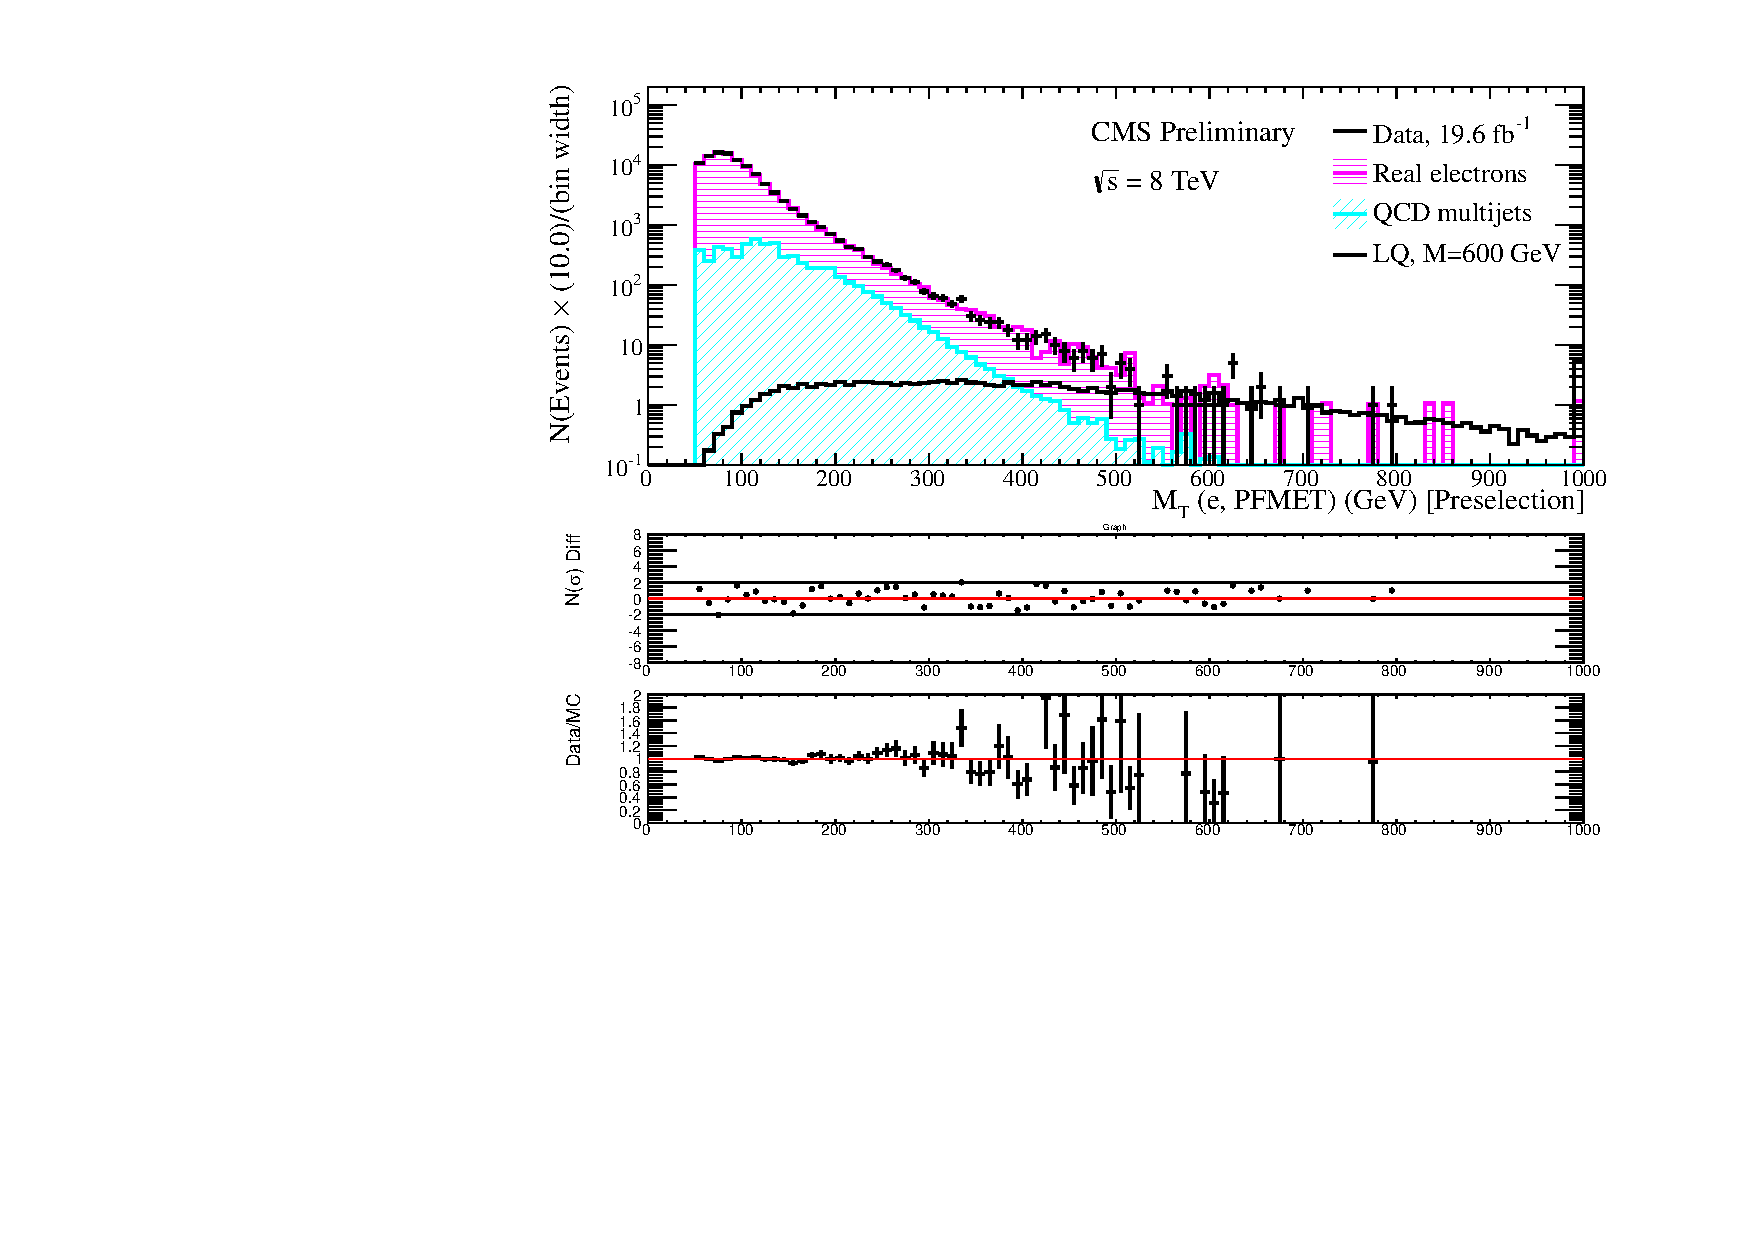
\includegraphics[width=0.875\textwidth]{fig/enu/muonbackground/MTenu_PAS_enujj.pdf}
\end{column}
\begin{column}{0.6\textwidth}
%% ST
\label{sec-1-6-4-1-2}

\centering
\ST at \enujj preselection
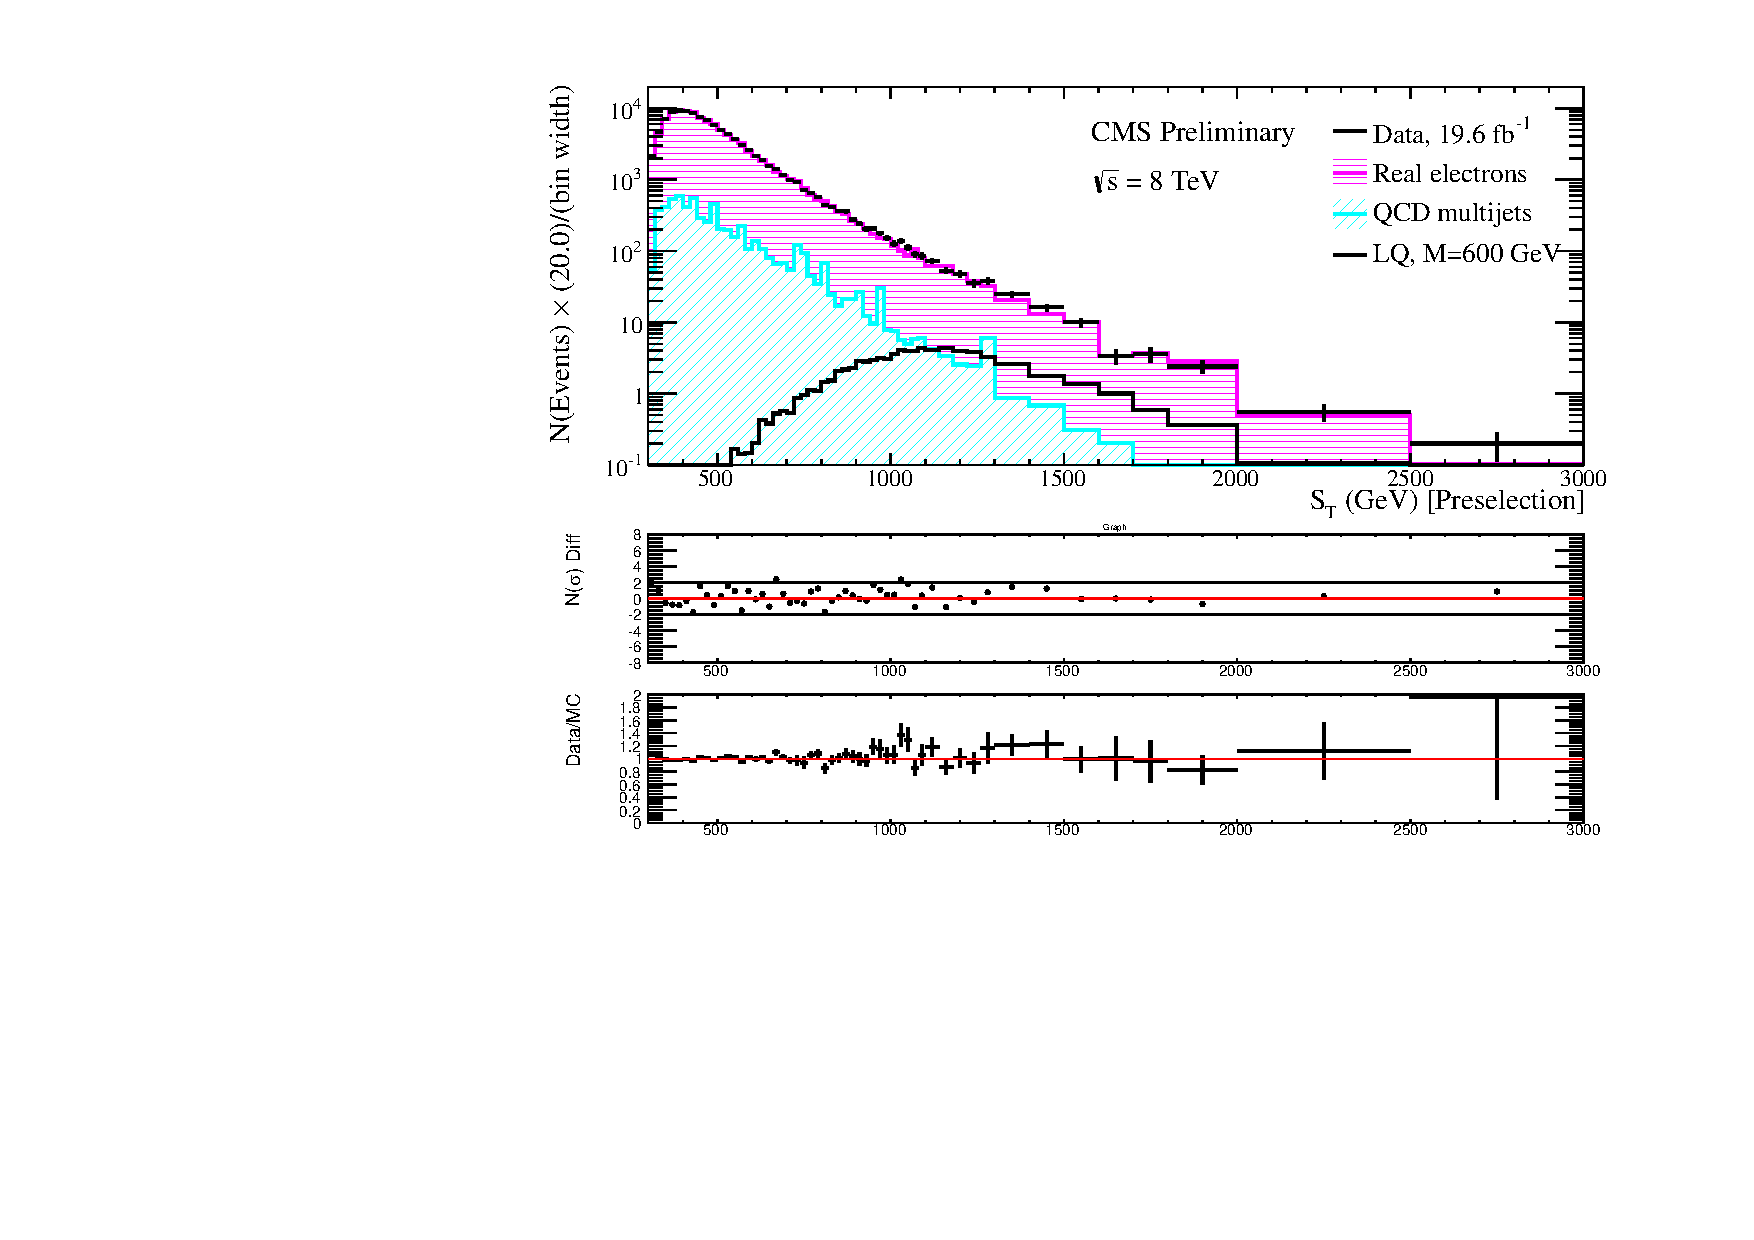
\includegraphics[width=0.875\textwidth]{fig/enu/muonbackground/sT_PAS_enujj.pdf}
\end{column}
\end{columns}
%% Text
\label{sec-1-6-4-2}

\begin{itemize}
\item "Real electrons": \enujj events with no fake electrons (modeled with \munujj)
\item \mt in \munujj events reweighted to match data
\end{itemize}
\end{frame}
\begin{frame}
\frametitle{Data-driven background using muons: \enujj (2/2)}
\label{sec-1-6-5}
%% Table
\label{sec-1-6-5-1}

\centering
\resizebox*{!}{0.6\textheight}{
\begin{tikzpicture}
\node (table) {
\begin{tabular}{| l | c | c | c | c | c |} 
  \hline 
  \hline 
$M_{LQ}$ & LQ Signal & Real electrons (from data) & QCD (from data) & Data & Total Background \\ 
  \hline 
  \hline 
Presel & - &  $ 99103.1 \pm 323.9 $ & $ 5950.5 \pm 20.1 $ &105164 & $ 105053.6 \pm 324.5 $ \\ 
  \hline 
300 &  $ 4641.6\pm 49.8 $ &  $ 2346.6 \pm 51.1 $ & $ 117.9 \pm 1.5 $ & 2455 &  $ 2464.50 \pm 51.11 $ \\ 
350 &  $ 2112.1\pm 21.1 $ &  $ 827.0 \pm 29.3 $ & $ 59.11 \pm 0.97 $ & 908 &  $ 886.15 \pm 29.31 $ \\ 
400 &  $ 945.8\pm 9.3 $ &  $ 343.0 \pm 18.4 $ & $ 32.88 \pm 0.69 $ & 413 &  $ 375.86 \pm 18.38 $ \\ 
450 &  $ 457.5\pm 4.5 $ &  $ 144.5 \pm 11.8 $ & $ 14.13 \pm 0.42 $ & 192 &  $ 158.64 \pm 11.81 $ \\ 
500 &  $ 226.7\pm 2.2 $ &  $ 77.8 \pm 8.6 $ & $ 7.76 \pm 0.30 $ & 83 &  $ 85.55 \pm 8.60 $ \\ 
550 &  $ 118.2\pm 1.2 $ &  $ 28.3 \pm 5.2 $ & $ 3.89 \pm 0.21 $ & 44 &  $ 32.18 \pm 5.17 $ \\ 
600 &  $ 64.65\pm 0.64 $ &  $ 13.2 \pm 3.5 $ & $ 2.29 \pm 0.17 $ & 28 &  $ 15.53 \pm 3.54 $ \\ 
650 &  $ 36.25\pm 0.36 $ &  $ 9.5 \pm 3.0 $ & $ 1.18 \pm 0.12 $ & 18 &  $ 10.65 \pm 3.00 $ \\ 
700 &  $ 21.18\pm 0.21 $ &  $ 4.7 \pm 2.1 $ & $ 0.85 \pm 0.10 $ & 6 &  $ 5.58 \pm 2.12 $ \\ 
750 &  $ 12.56\pm 0.12 $ &  $ 1.8 \pm 1.3 $ & $ 0.514 \pm 0.091 $ & 4 &  $ 2.32 \pm 1.28 $ \\ 
800 &  $ 7.412\pm 0.073 $ &  $ 0.90 \pm 0.90 $ & $ 0.317 \pm 0.067 $ & 3 &  $ 1.22 \pm 0.90 $ \\ 
850 &  $ 4.591\pm 0.045 $ &  $ 0.000_{-0.00}^{1.14} $ &  $ 0.117 \pm 0.029 $ & 2 &  $ 0.117_{-0.029}^{+1.140}$ \\ 
900 &  $ 2.853\pm 0.028 $ &  $ 0.000_{-0.00}^{1.14} $ &  $ 0.076 \pm 0.024 $ & 1 &  $ 0.076_{-0.024}^{+1.140}$ \\ 
950 &  $ 1.791\pm 0.017 $ &  $ 0.000_{-0.00}^{1.14} $ &  $ 0.069 \pm 0.023 $ & 1 &  $ 0.069_{-0.023}^{+1.140}$ \\ 
1000 &  $ 1.272\pm 0.011 $ &  $ 0.000_{-0.00}^{1.14} $ &  $ 0.069 \pm 0.023 $ & 1 &  $ 0.069_{-0.023}^{+1.140}$ \\ 
1050 &  $ 0.8788\pm 0.0074 $ &  $ 0.000_{-0.00}^{1.14} $ &  $ 0.069 \pm 0.023 $ & 1 &  $ 0.069_{-0.023}^{+1.140}$ \\ 
1100 &  $ 0.6063\pm 0.0049 $ &  $ 0.000_{-0.00}^{1.14} $ &  $ 0.069 \pm 0.023 $ & 1 &  $ 0.069_{-0.023}^{+1.140}$ \\ 
1150 &  $ 0.4196\pm 0.0032 $ &  $ 0.000_{-0.00}^{1.14} $ &  $ 0.069 \pm 0.023 $ & 1 &  $ 0.069_{-0.023}^{+1.140}$ \\ 
1200 &  $ 0.2894\pm 0.0021 $ &  $ 0.000_{-0.00}^{1.14} $ &  $ 0.069 \pm 0.023 $ & 1 &  $ 0.069_{-0.023}^{+1.140}$ \\ 
  \hline 
  \hline 
\end{tabular}
};
\draw [red,ultra thick,rounded corners]
($(table.south west) !.515! (table.north west)$)
rectangle 
($(table.south east) !.565! (table.north east)$);    
\draw [red,ultra thick,rounded corners]
($(table.north east) !.285! (table.north west)$)
rectangle 
($(table.south east) !0.! (table.north west)$);    
\end{tikzpicture}
}
%% Text
\label{sec-1-6-5-2}

\begin{itemize}
\item 18 events observed at M(LQ) = 650
\item MC analysis predicts $7.54 \pm 1.20$ (stat) $\pm$ 0.52 (syst)
\item DD analysis (this table) predicts $10.65 \pm 3.00$ (stat)
\end{itemize}
\end{frame}
\begin{frame}
\frametitle{Data-driven background using muons: limits}
\label{sec-1-6-6}
\begin{columns} % Plots
\label{sec-1-6-6-1}
\begin{column}{0.5\textwidth}
%% eejj limit, no syst
\label{sec-1-6-6-1-1}

\centering
$\beta = 1.0$: \eejj analysis, $\mu$-bkgd.
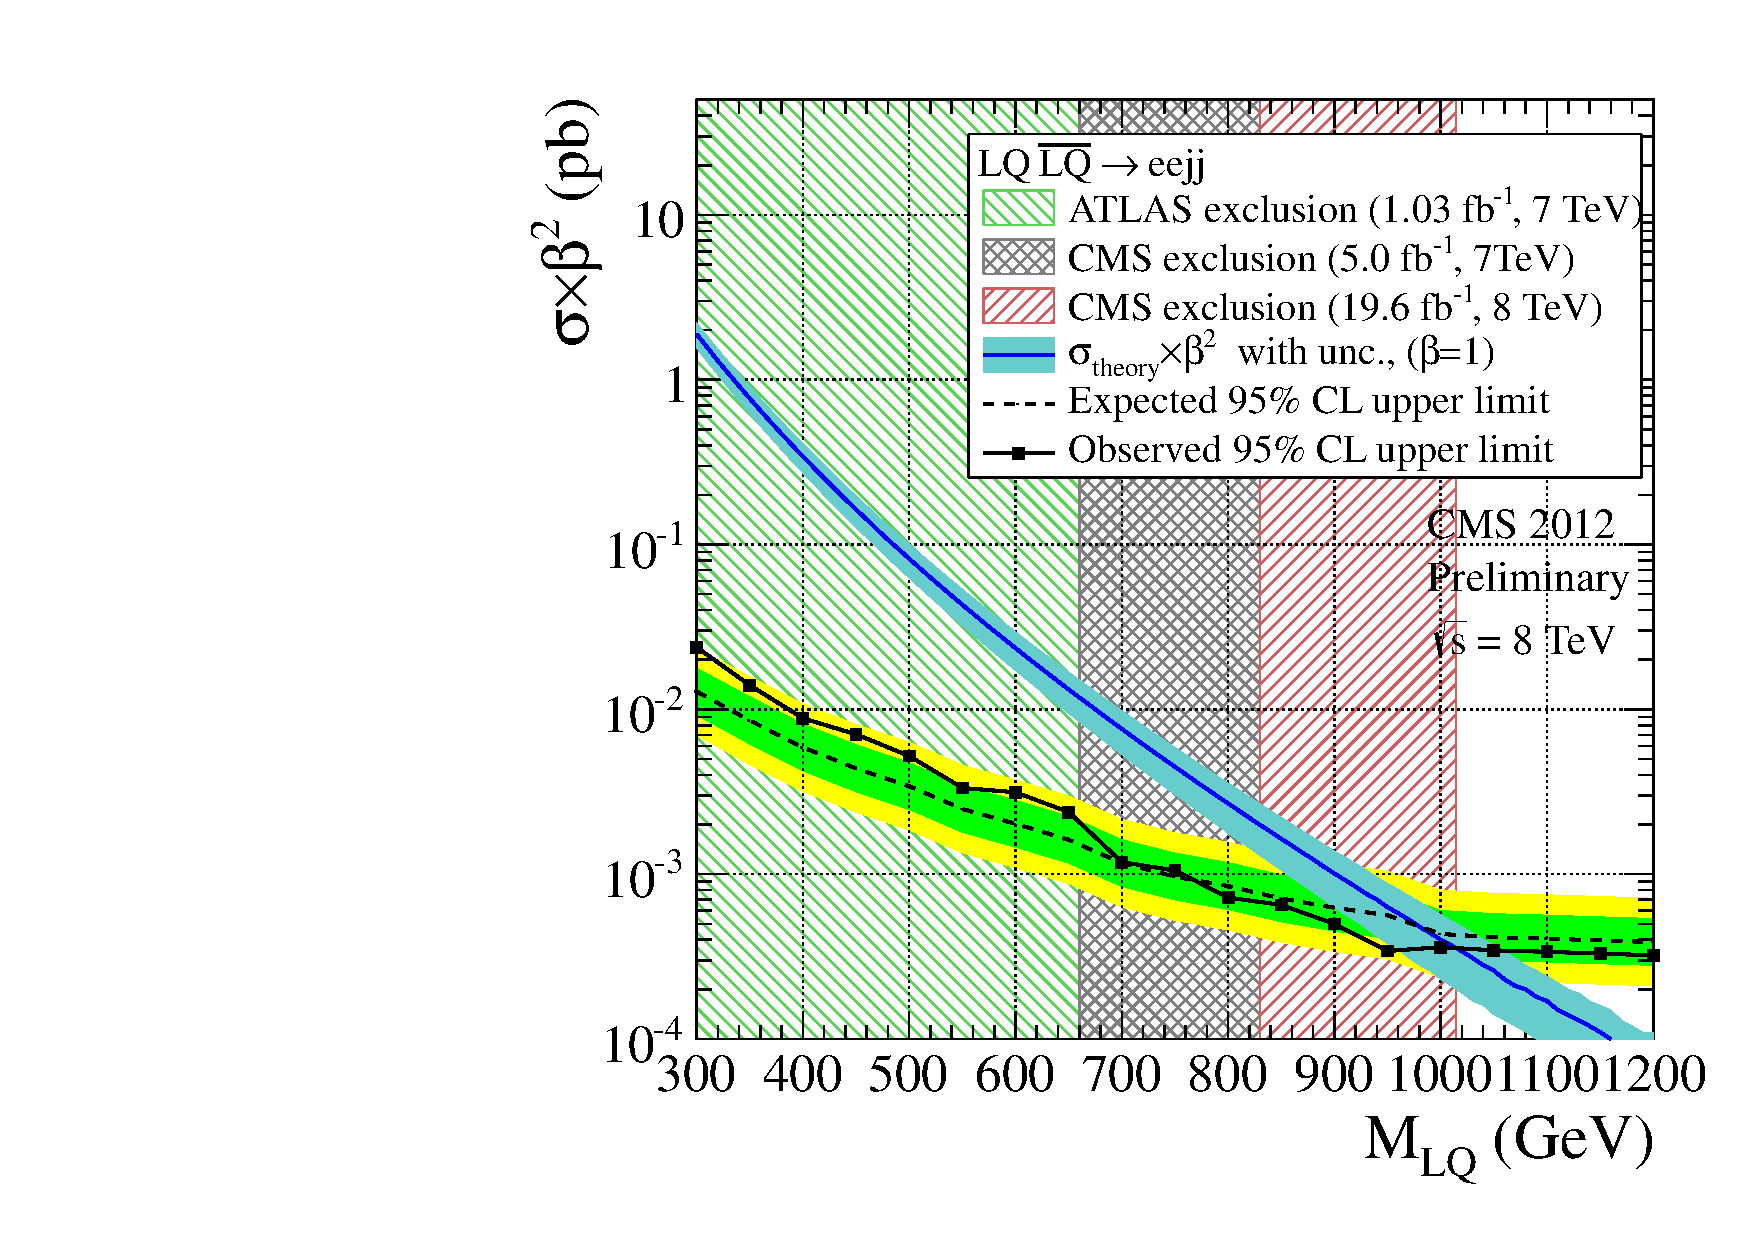
\includegraphics[width=0.875\textwidth]{fig/limits/BR_Sigma_EE_muonBackground.pdf}
\end{column}
\begin{column}{0.5\textwidth}
%% enujj limit, no syst
\label{sec-1-6-6-1-2}

\centering
$\beta = 0.5$: \enujj analysis, $\mu$-bkgd.
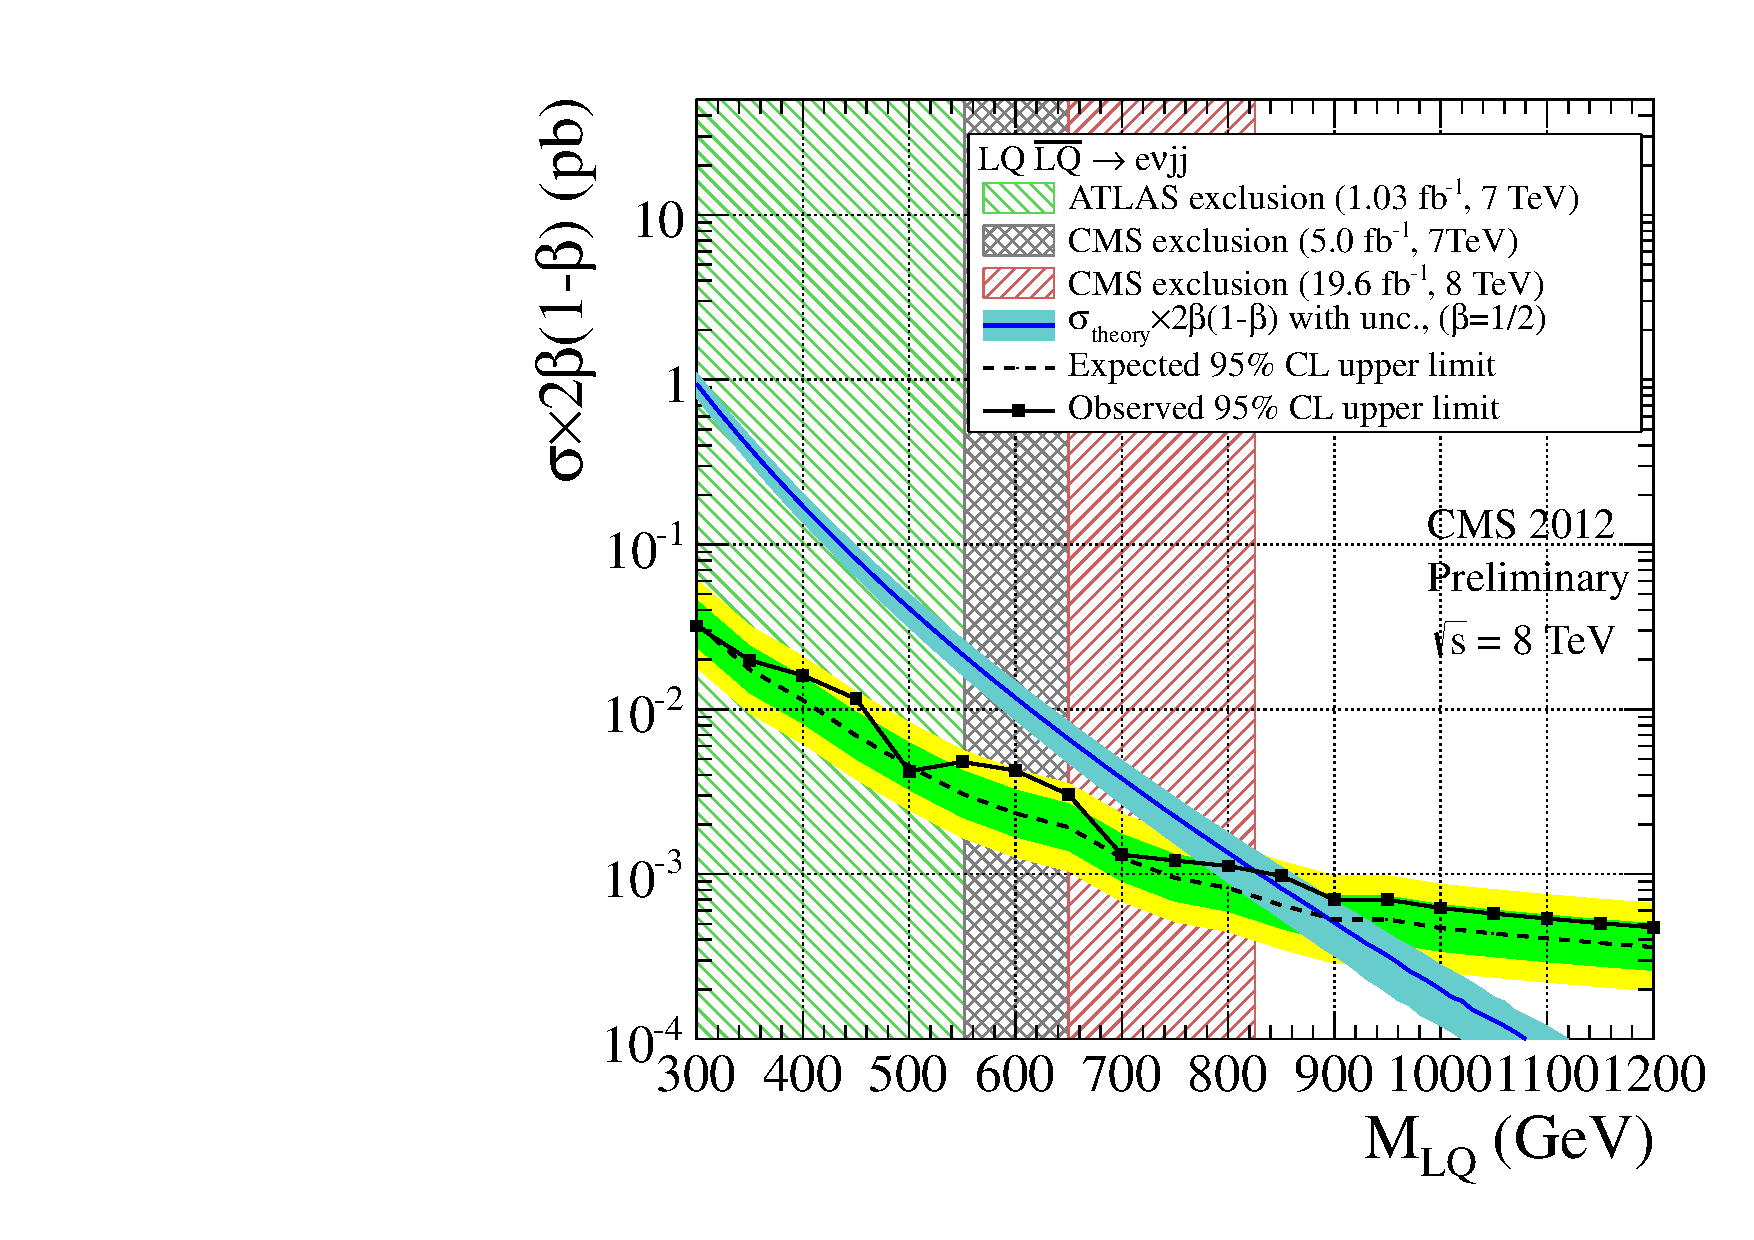
\includegraphics[width=0.875\textwidth]{fig/limits/BR_Sigma_ENu_muonBackground.pdf}
\end{column}
\end{columns}
%% Notes
\label{sec-1-6-6-2}

\begin{itemize}
\item Expected limits: $M_{LQ} < \eejjExpectedLimitMuon$ $(\enujjExpectedLimitMuon)$ GeV for \eejj (\enujj)
\item Observed limits: $M_{LQ} < \eejjObservedLimitMuon$ $(\enujjObservedLimitMuon)$ GeV for \eejj (\enujj)
\end{itemize}
\end{frame}
\begin{frame}
\frametitle{Data-driven background using muons: conclusion}
\label{sec-1-6-7}
%% Text
\label{sec-1-6-7-1}

\ChangeItemFont{\footnotesize}{\footnotesize}{\footnotesize}
\begin{itemize}
\item Data-driven predictions agree with MC predictions at final selection ($M_{LQ} = 650$ GeV) within stat. uncertainties in both analyses
\item Conclusion: \alert{Data-driven background prediction confirms MC background prediction}
\item However:
\begin{itemize}
\item Data-driven prediction mean values are higher than MC
\item Data-driven stat uncertainty is larger than MC
\item So the significance of the excess with data-driven background estimates is less than the significance with MC background estimates
\item And the sensitivity of the analysis with data-driven background estimates is worse than the sensitivity with MC background estimates
\end{itemize}
\end{itemize}
\end{frame}
\subsection{Comparison with LQ2}
\label{sec-1-7}
\begin{frame}
\frametitle{Comparison with LQ2}
\label{sec-1-7-1}
%% Table
\label{sec-1-7-1-1}

\centering
\resizebox*{!}{0.7\textheight}{
\begin{tabular}{| c | c | c | c | c |}
\hline 
\hline 
$M_{LQ}$ & $eejj$ Total Background & $eejj$ Data & $\mu\mu jj$ Total Background & $\mu\mu jj$ Data \\ 
\hline 
\hline
300   &  $ 1444.96 \pm 13.65 $ & 1539 & 1415  $\pm$ 20   $\pm$ 45  (syst)  & 1461 \\        
350   &  $ 726.71 \pm 9.78 $   & 759  & 730   $\pm$ 15   $\pm$ 16  (syst)  & 714 \\             
400   &  $ 399.70 \pm 7.23 $   & 423  & 384.8 $\pm$ 10.7 $\pm$ 9.3 (syst)  & 394 \\         
450   &  $ 208.02 \pm 5.18 $   & 235  & 205.3 $\pm$ 7.6  $\pm$ 5.5 (syst)  & 210 \\         
500   &  $ 118.74 \pm 4.00 $   & 145  & 121.6 $\pm$ 5.7  $\pm$ 4.8 (syst)  & 128 \\         
550   &  $ 71.50 \pm 3.25 $    & 94   & 68.1  $\pm$ 4.2  $\pm$ 2.7 (syst)  & 75 \\          
600   &  $ 42.44 \pm 2.40 $    & 67   & 44.7  $\pm$ 3.4  $\pm$ 2.0 (syst)  & 44 \\          
650   &  $ 26.99 \pm 1.93 $    & 43   & 28    $\pm$ 2.6  $\pm$ 1.3 (syst)  & 24 \\          
700   &  $ 16.42 \pm 1.52 $    & 22   & 18.6  $\pm$ 2.2  $\pm$ 1.3 (syst)  & 15 \\          
750   &  $ 10.27 \pm 1.23 $    & 14   & 9.32  $ _{-1.22}^{+1.29}$   $\pm$ 0.87 (syst)  &       11 \\          
800   &  $ 5.08 \pm 0.77 $     & 10   & 6.53  $ _{-1.13}^{+1.2}$   $\pm$ 0.85 (syst)  &        9 \\           
850   &  $ 2.97 \pm 0.54 $     & 4    & 3.88  $ _{-0.92}^{+1.0}$   $\pm$ 0.67 (syst)  &        5 \\             
900   &  $ 1.71 \pm 0.41 $     & 3    & 1.47  $ _{-0.37}^{+0.81}$   $\pm$ 0.43 (syst)  &       3 \\           
950   &  $ 1.04 \pm 0.31 $     & 1    & 0.83  $ _{-0.26}^{+0.91}$   $\pm$ 0.29 (syst)  &       1 \\           
1000  &  $ 0.62 \pm 0.24 $     & 0    & 0.383 $ _{-0.171}^{+0.894}$   $\pm$ 0.031 (syst)  &   0 \\             
1050  &  $ 0.62 \pm 0.24 $     & 0    & 0.383 $ _{-0.171}^{+0.894}$   $\pm$ 0.031 (syst)  &   0 \\             
1100  &  $ 0.62 \pm 0.24 $     & 0    & 0.383 $ _{-0.171}^{+0.894}$   $\pm$ 0.031 (syst)  &   0 \\             
1150  &  $ 0.62 \pm 0.24 $     & 0    & 0.383 $ _{-0.171}^{+0.894}$   $\pm$ 0.031 (syst)  &   0 \\             
1200  &  $ 0.62 \pm 0.24 $     & 0    & 0.383 $ _{-0.171}^{+0.894}$   $\pm$ 0.031 (syst)  &   0 \\             
\hline
\hline 
\end{tabular}
}
%% Text
\label{sec-1-7-1-2}

\begin{itemize}
\scriptsize
\item Apply \ST, \mejmin, and \mll cuts from LQ2 (\texttt{EXO-12-042})
\item \eejj bkgd prediction, \mumujj bkgd prediction, and \mumujj data agree well
\item \alert{Discrepancy comes from \eejj data}
\end{itemize}
\end{frame}
\subsection{Electron $\eta$ vs. $\phi$}
\label{sec-1-8}
\begin{frame}
\frametitle{Electron $\eta$ vs. $\phi$}
\label{sec-1-8-1}
\begin{columns} % Columns
\label{sec-1-8-1-1}
\begin{column}{0.5\textwidth}
%% eejj
\label{sec-1-8-1-1-1}

\centering
Events passing \eejj \\
$M_{LQ} = 650$ GeV selection
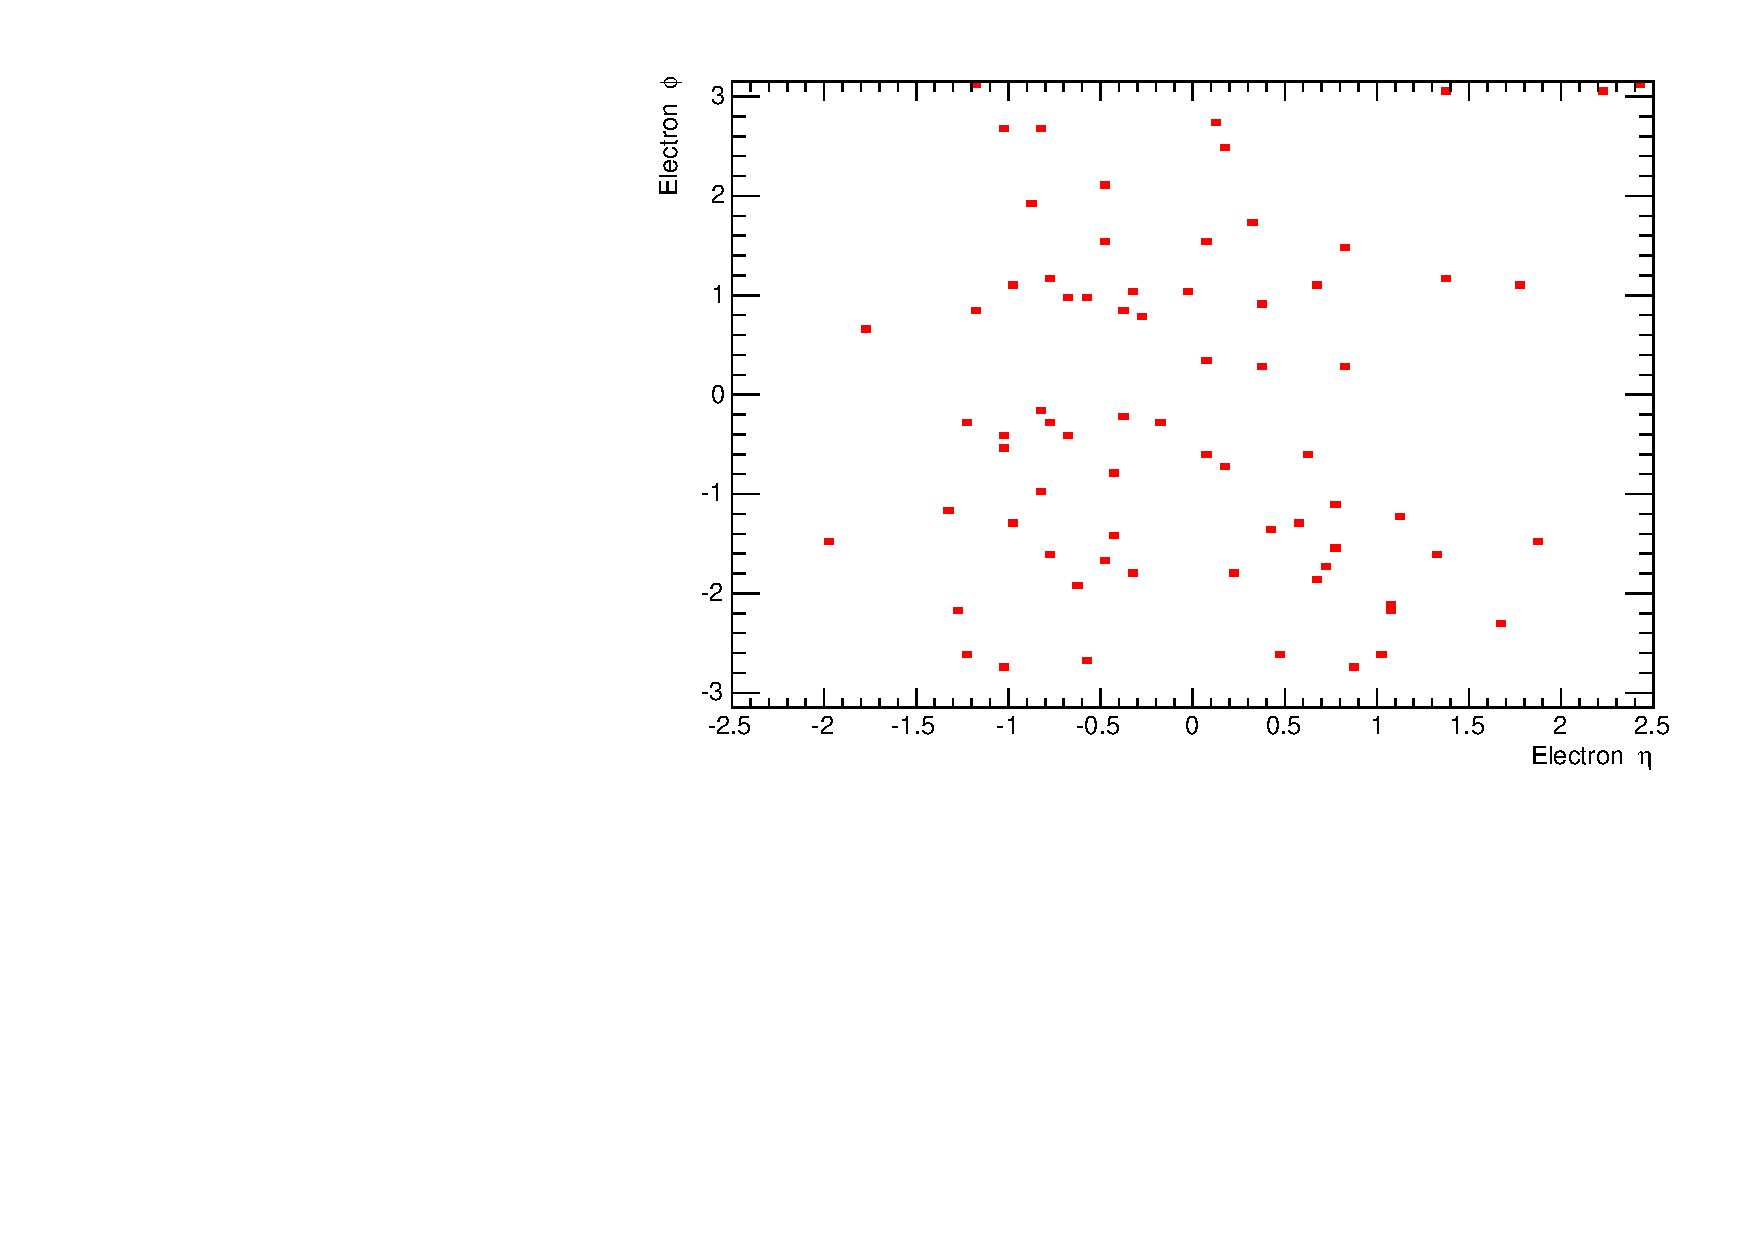
\includegraphics[width=\textwidth]{fig/ee/extra/eejj_electron_map.pdf}
\end{column}
\begin{column}{0.5\textwidth}
%% enujj
\label{sec-1-8-1-1-2}

\centering
Events passing \enujj \\
$M_{LQ} = 650$ GeV selection
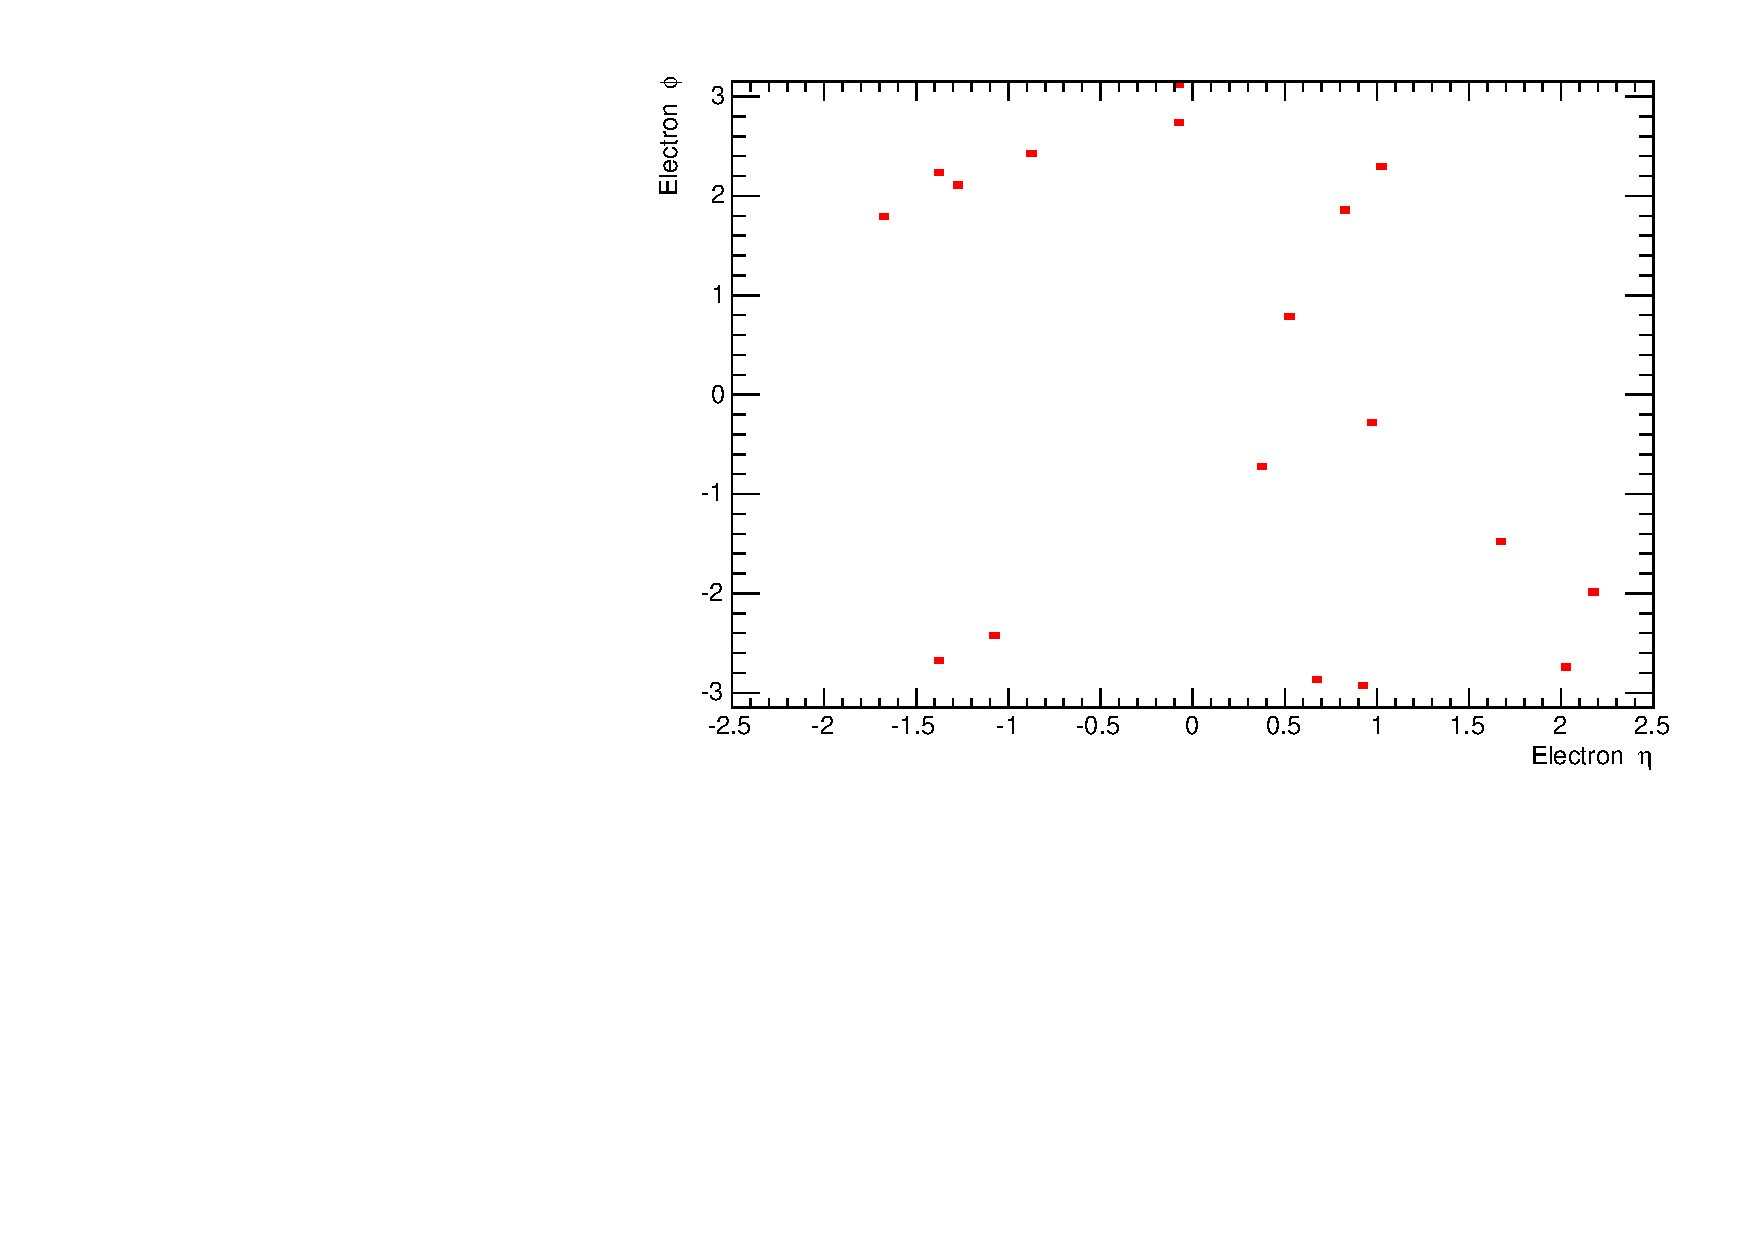
\includegraphics[width=\textwidth]{fig/enu/extra/enujj_electron_map.pdf}
\end{column}
\end{columns}
%% Note
\label{sec-1-8-1-2}

\small
\centering
Electrons in events passing final selection in both analyses are evenly distributed in the ECAL
\normalsize
\end{frame}
\subsection{Reweighting study}
\label{sec-1-9}
\begin{frame}
\frametitle{\met and \mt before reweighting}
\label{sec-1-9-1}
\begin{columns} % Columns
\label{sec-1-9-1-1}
\begin{column}{0.6\textwidth}
%% \met
\label{sec-1-9-1-1-1}

\centering
\met before reweighting
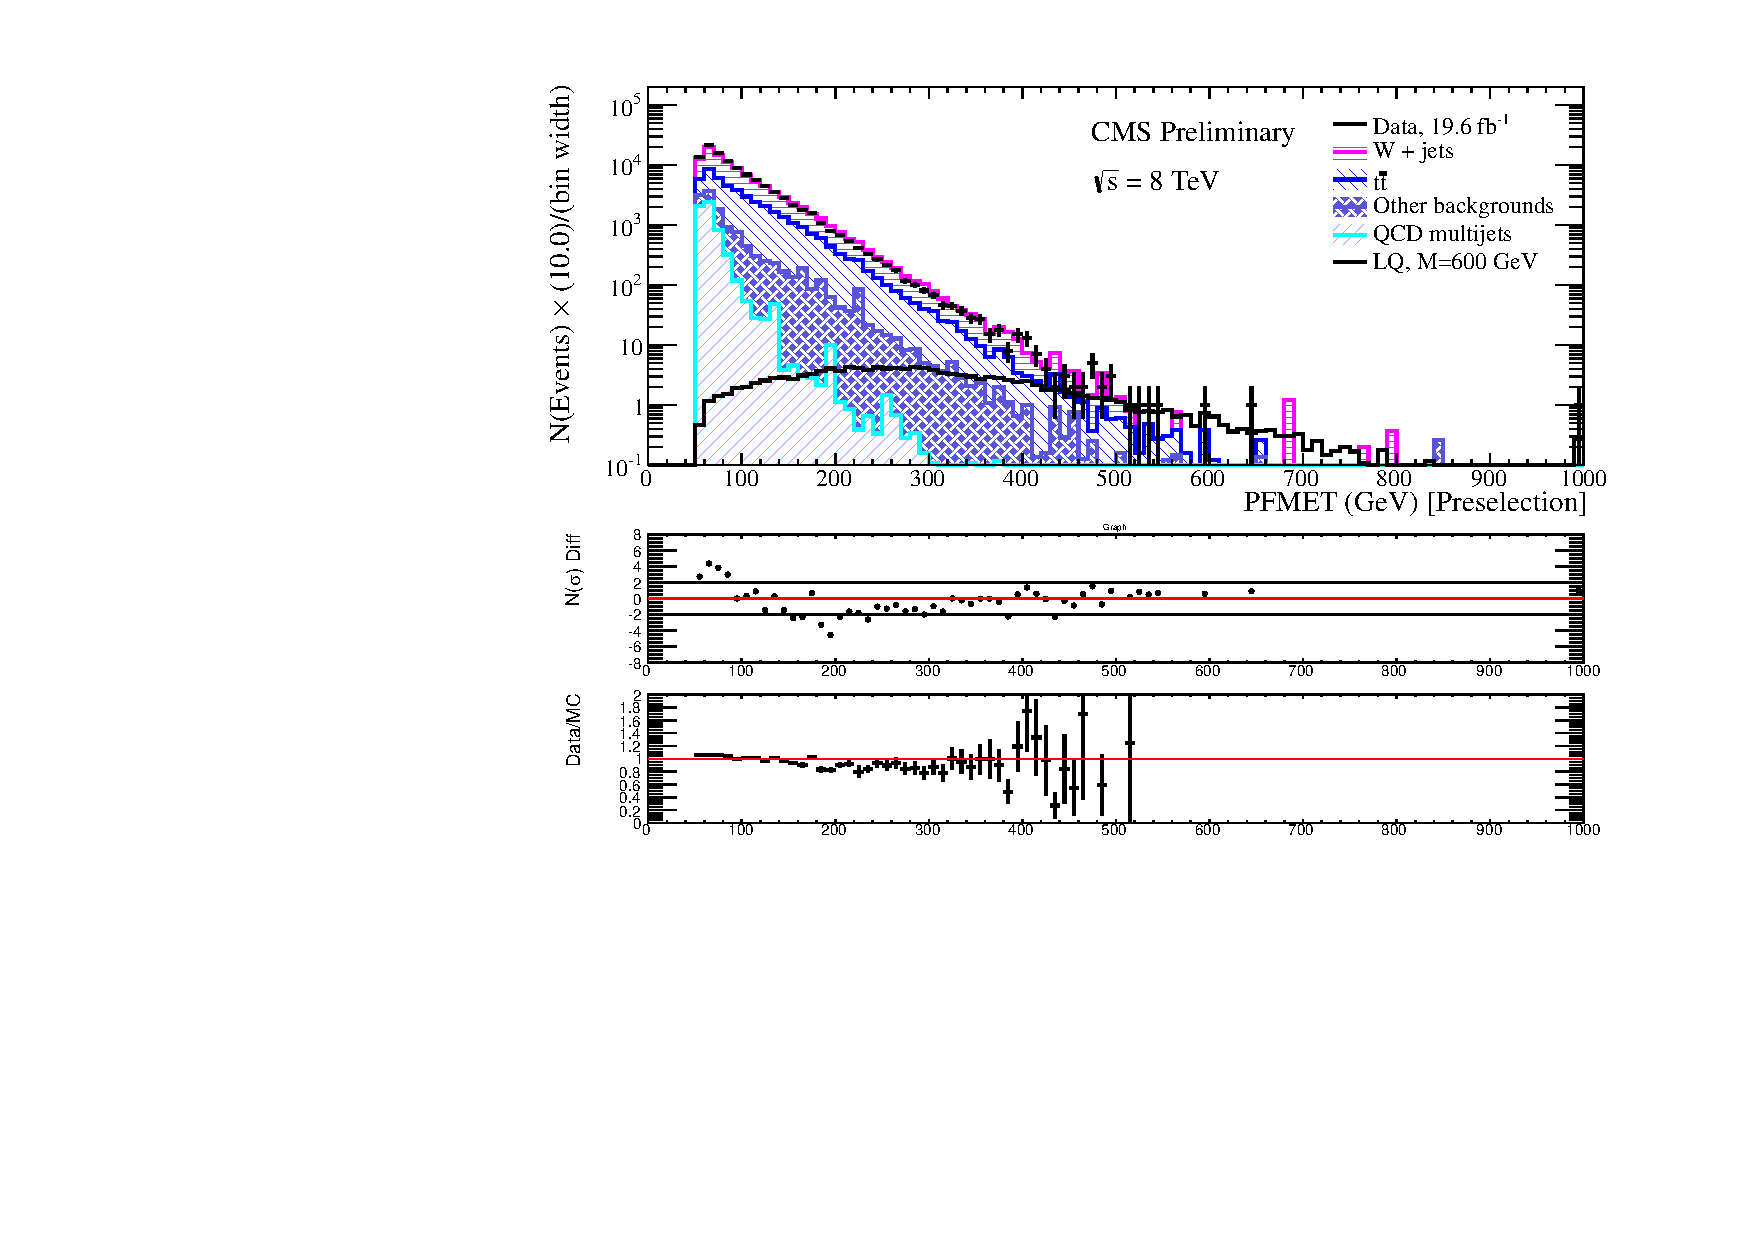
\includegraphics[width=\textwidth]{fig/enu/preselection/MET_PAS_enujj.pdf}
\end{column}
\begin{column}{0.6\textwidth}
%% \mt
\label{sec-1-9-1-1-2}

\centering
\mt before reweighting
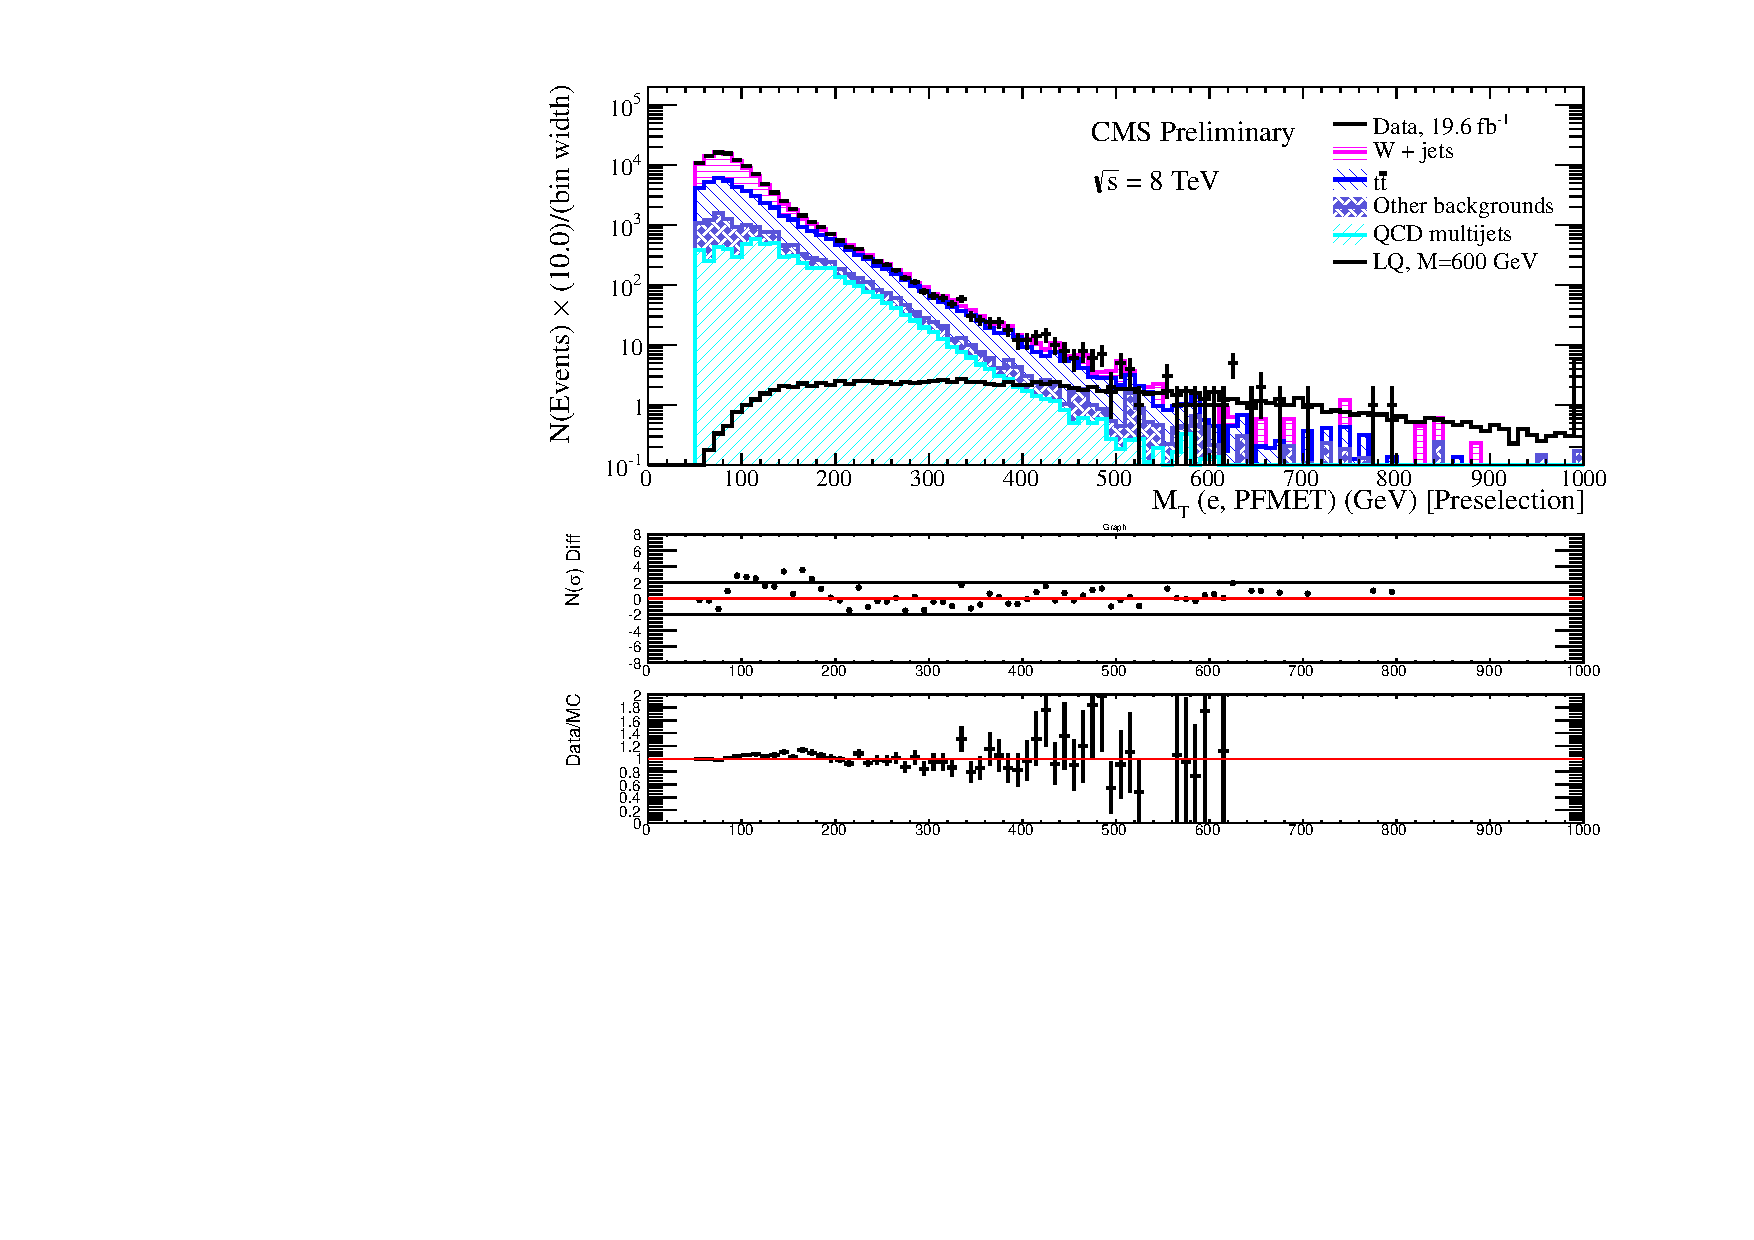
\includegraphics[width=\textwidth]{fig/enu/preselection/MTenu_PAS_enujj.pdf}
\end{column}
\end{columns}
%% Text
\label{sec-1-9-1-2}

\small
\centering
Can we improve agreement in these distributions by reweighting?
\end{frame}
\begin{frame}
\frametitle{Reweighting method}
\label{sec-1-9-2}
%% Text
\label{sec-1-9-2-1}

\begin{itemize}
\item Find weight functions for both \met and \mt at \enujj preselection:
\begin{enumerate}
\item Do not apply any \wjets or \ttbar rescaling
\item Find and apply weight function for \met first
\item Then find and apply weight function for \mt
\item Finally, find and apply new \wjets and \ttbar rescaling
\end{enumerate}
\item Compare \mt and \met dists. before and after reweighting
\item Repeat final selection for both \eejj and \enujj analysis
\end{itemize}
\end{frame}
\begin{frame}
\frametitle{Find \met function}
\label{sec-1-9-3}
\begin{columns} % Columns
\label{sec-1-9-3-1}
\begin{column}{0.6\textwidth}
%% \met before reweighting
\label{sec-1-9-3-1-1}

\centering
\met before reweighting
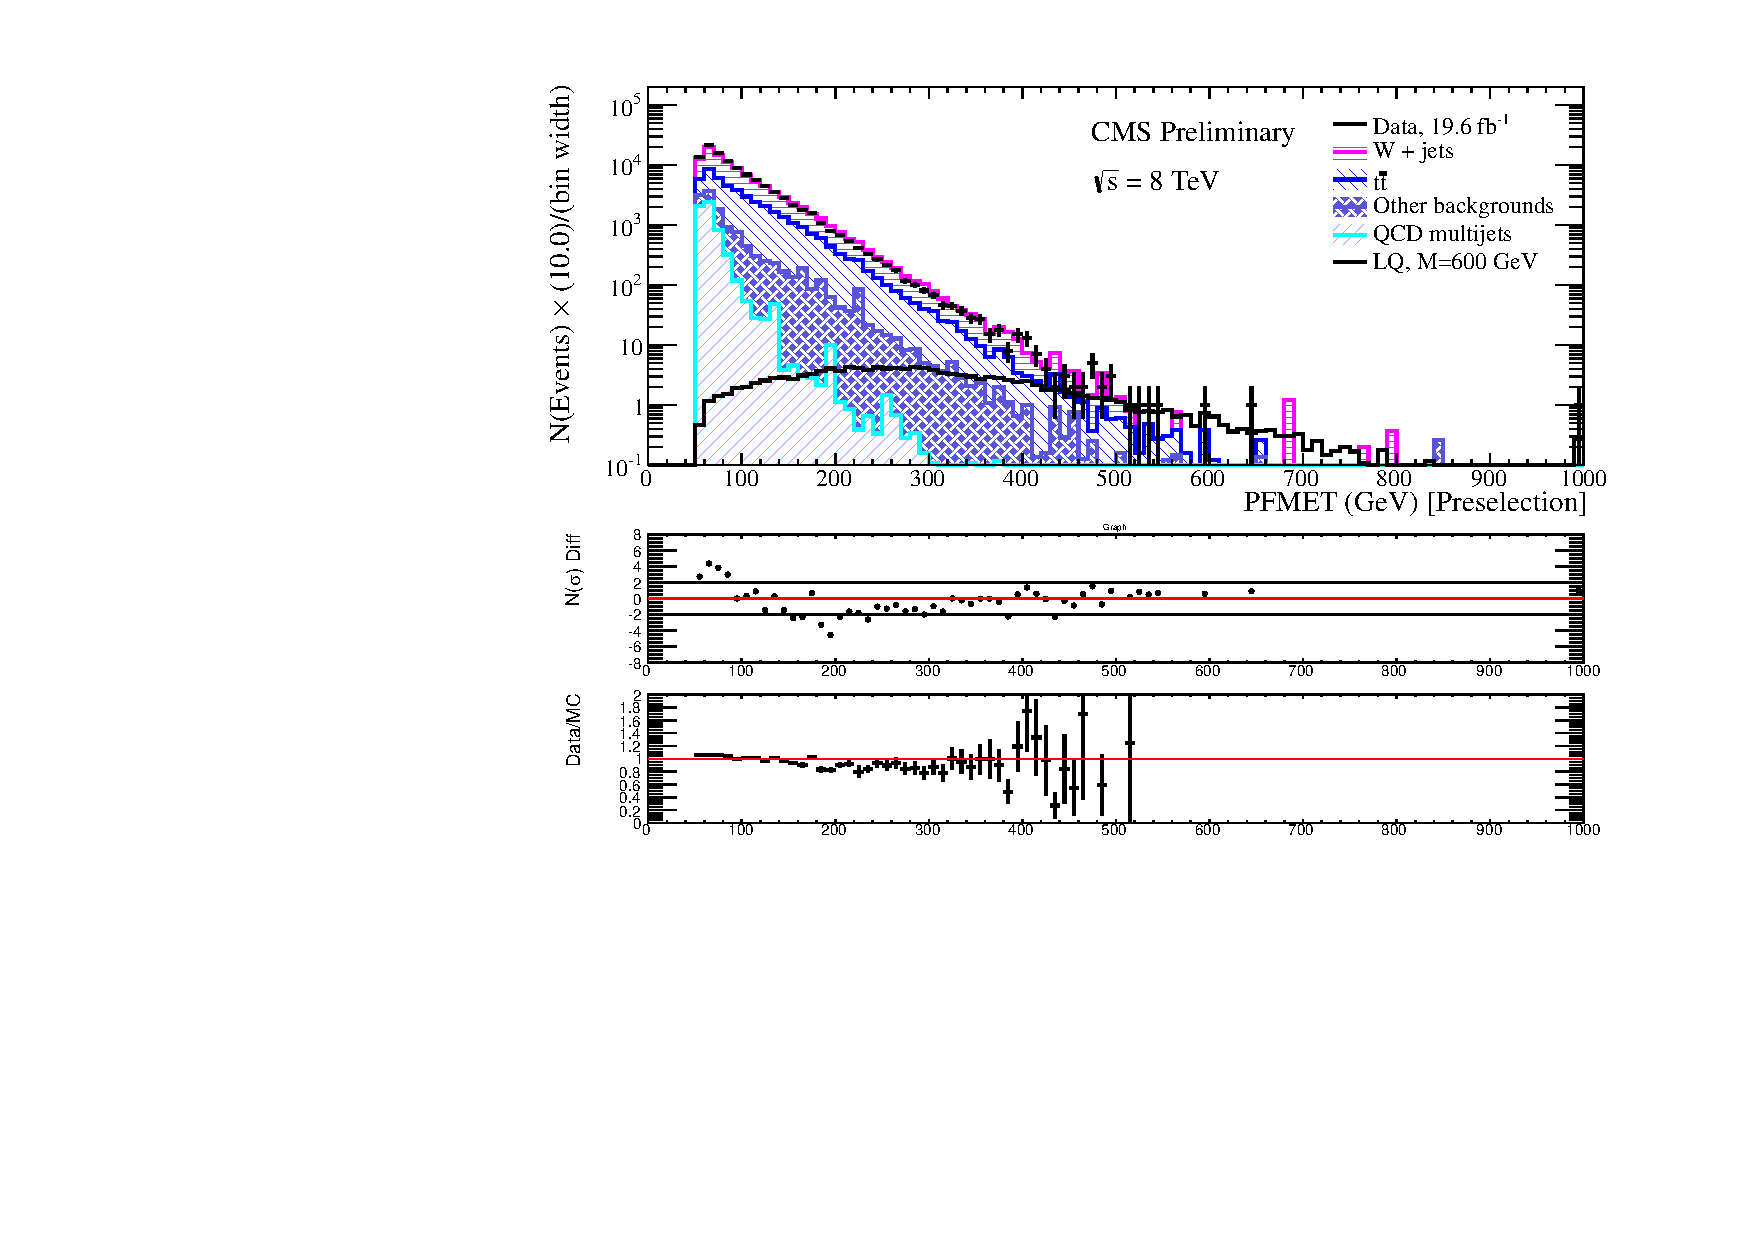
\includegraphics[width=\textwidth]{fig/enu/preselection/MET_PAS_enujj.pdf}
\end{column}
\begin{column}{0.6\textwidth}
%% Ratio
\label{sec-1-9-3-1-2}

\centering
\met reweighting function
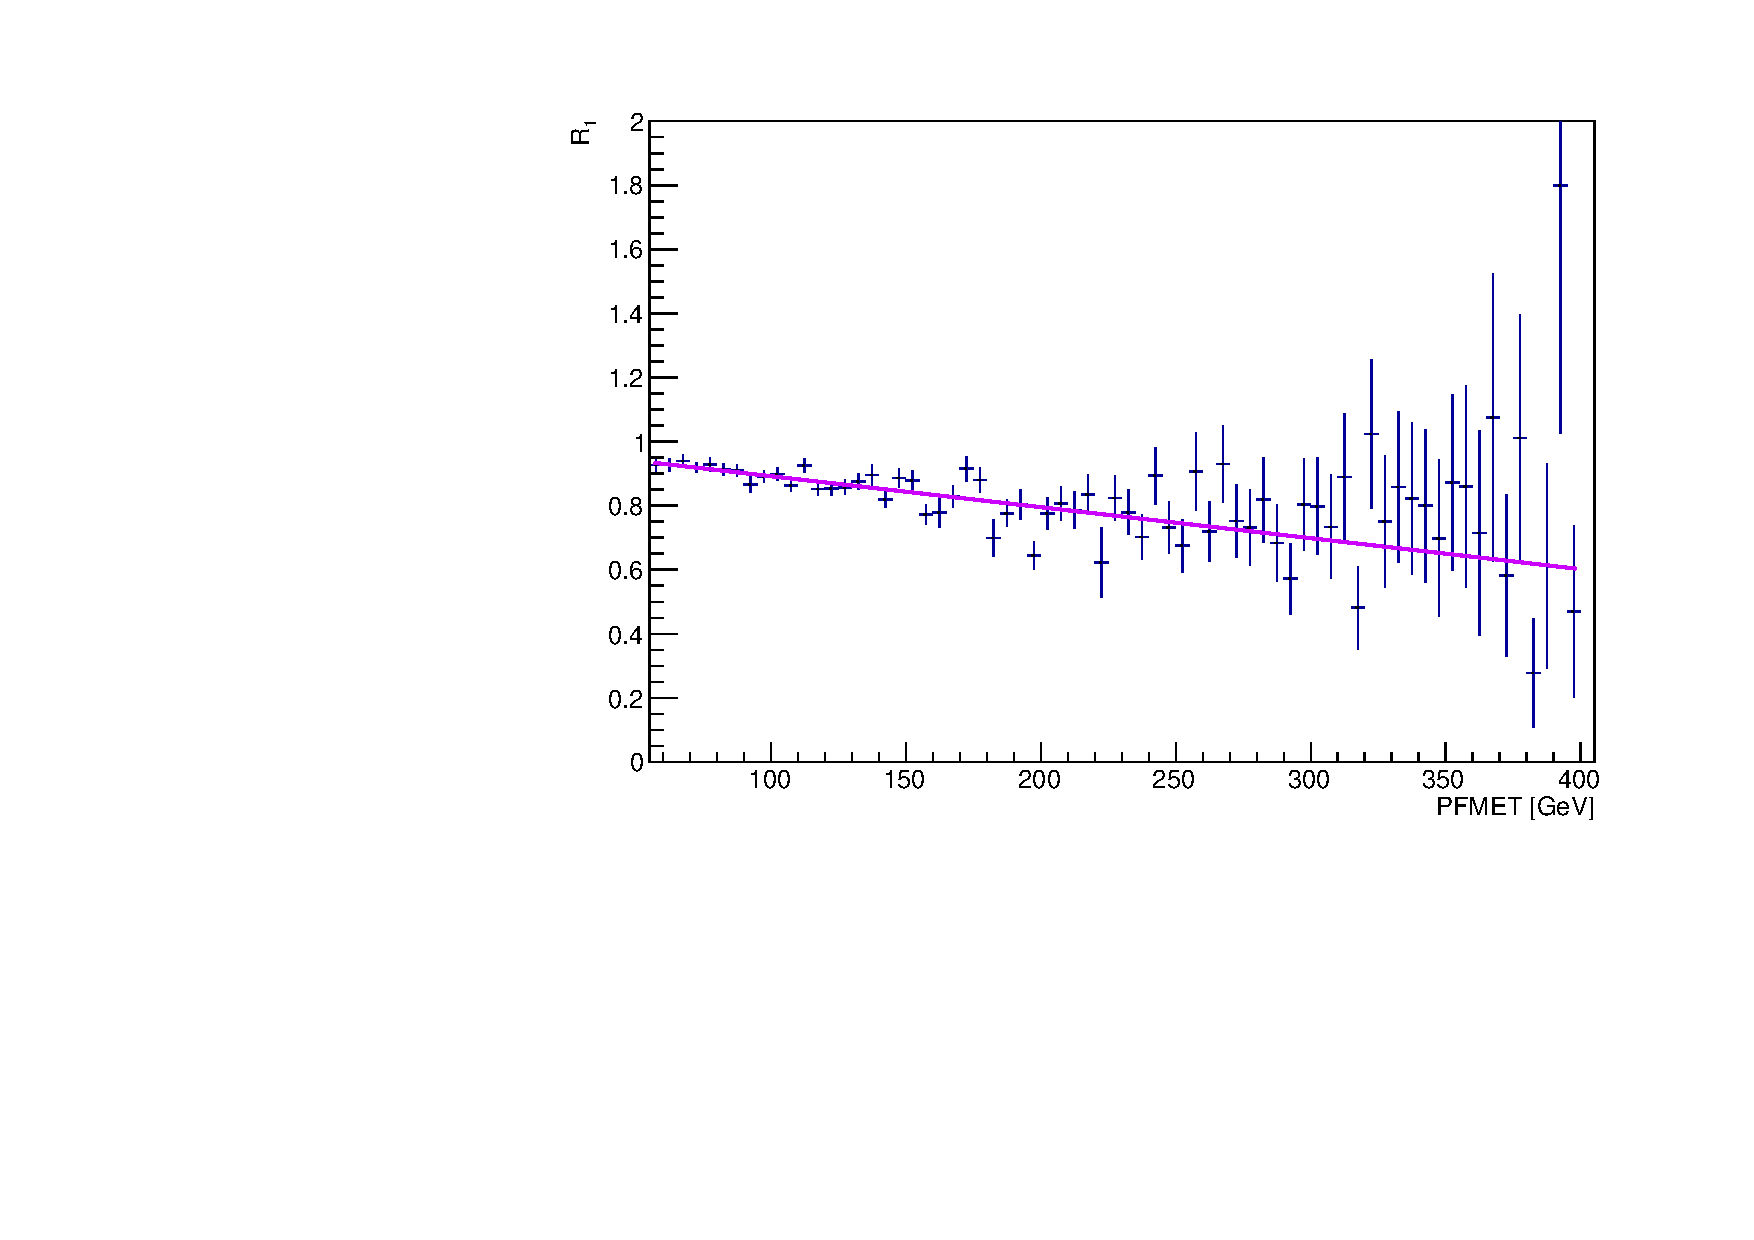
\includegraphics[width=\textwidth]{fig/enu/reweight/canvas_met.pdf}
\end{column}
\end{columns}
%% Text
\label{sec-1-9-3-2}

\centering
\resizebox{!}{0.2\textheight}{\vbox{
Get reweighting function by fitting:
\begin{equation*}
\mathcal{R}_1(\met) = \frac{\text{N}_{i,\text{Data}}(\met) - \text{N}_{i,\text{QCD}}(\met)}{\text{N}_{i,\text{W}+\text{jets}}(\met) + \text{N}_{i,\ttbar}(\met) + \text{N}_{i,\text{Other}}(\met)}
\end{equation*}
}}
\end{frame}
\begin{frame}
\frametitle{\met function details}
\label{sec-1-9-4}
%% Text
\label{sec-1-9-4-1}

\centering
\begin{itemize}
\item Use the following linear fit function to define \met reweighting:
\end{itemize}
\centering
\begin{equation*}
w_1(\met) = a_0 + a_1 \cdot \met
\end{equation*}
\begin{itemize}
\item Fit returns the following parameters:
\end{itemize}
\resizebox{\textwidth}{!}{
\begin{tabular}{|c|c|c|c|}
\hline
Parameter symbol & Parameter title & Mean value & Uncertainty \\
\hline
\hline
$a_0$    & Linear offset     & 0.989 & 0.0112 \\
$a_1$    & Linear slope      & $-9.67 \cdot 10^{-4}$ & $8.86 \cdot 10^{-5}$ \\
\hline
\end{tabular}
}
\end{frame}
\begin{frame}
\frametitle{Apply \met function}
\label{sec-1-9-5}
\begin{columns} % Columns
\label{sec-1-9-5-1}
\begin{column}{0.6\textwidth}
%% \met
\label{sec-1-9-5-1-1}

\centering
\met after \met reweighting
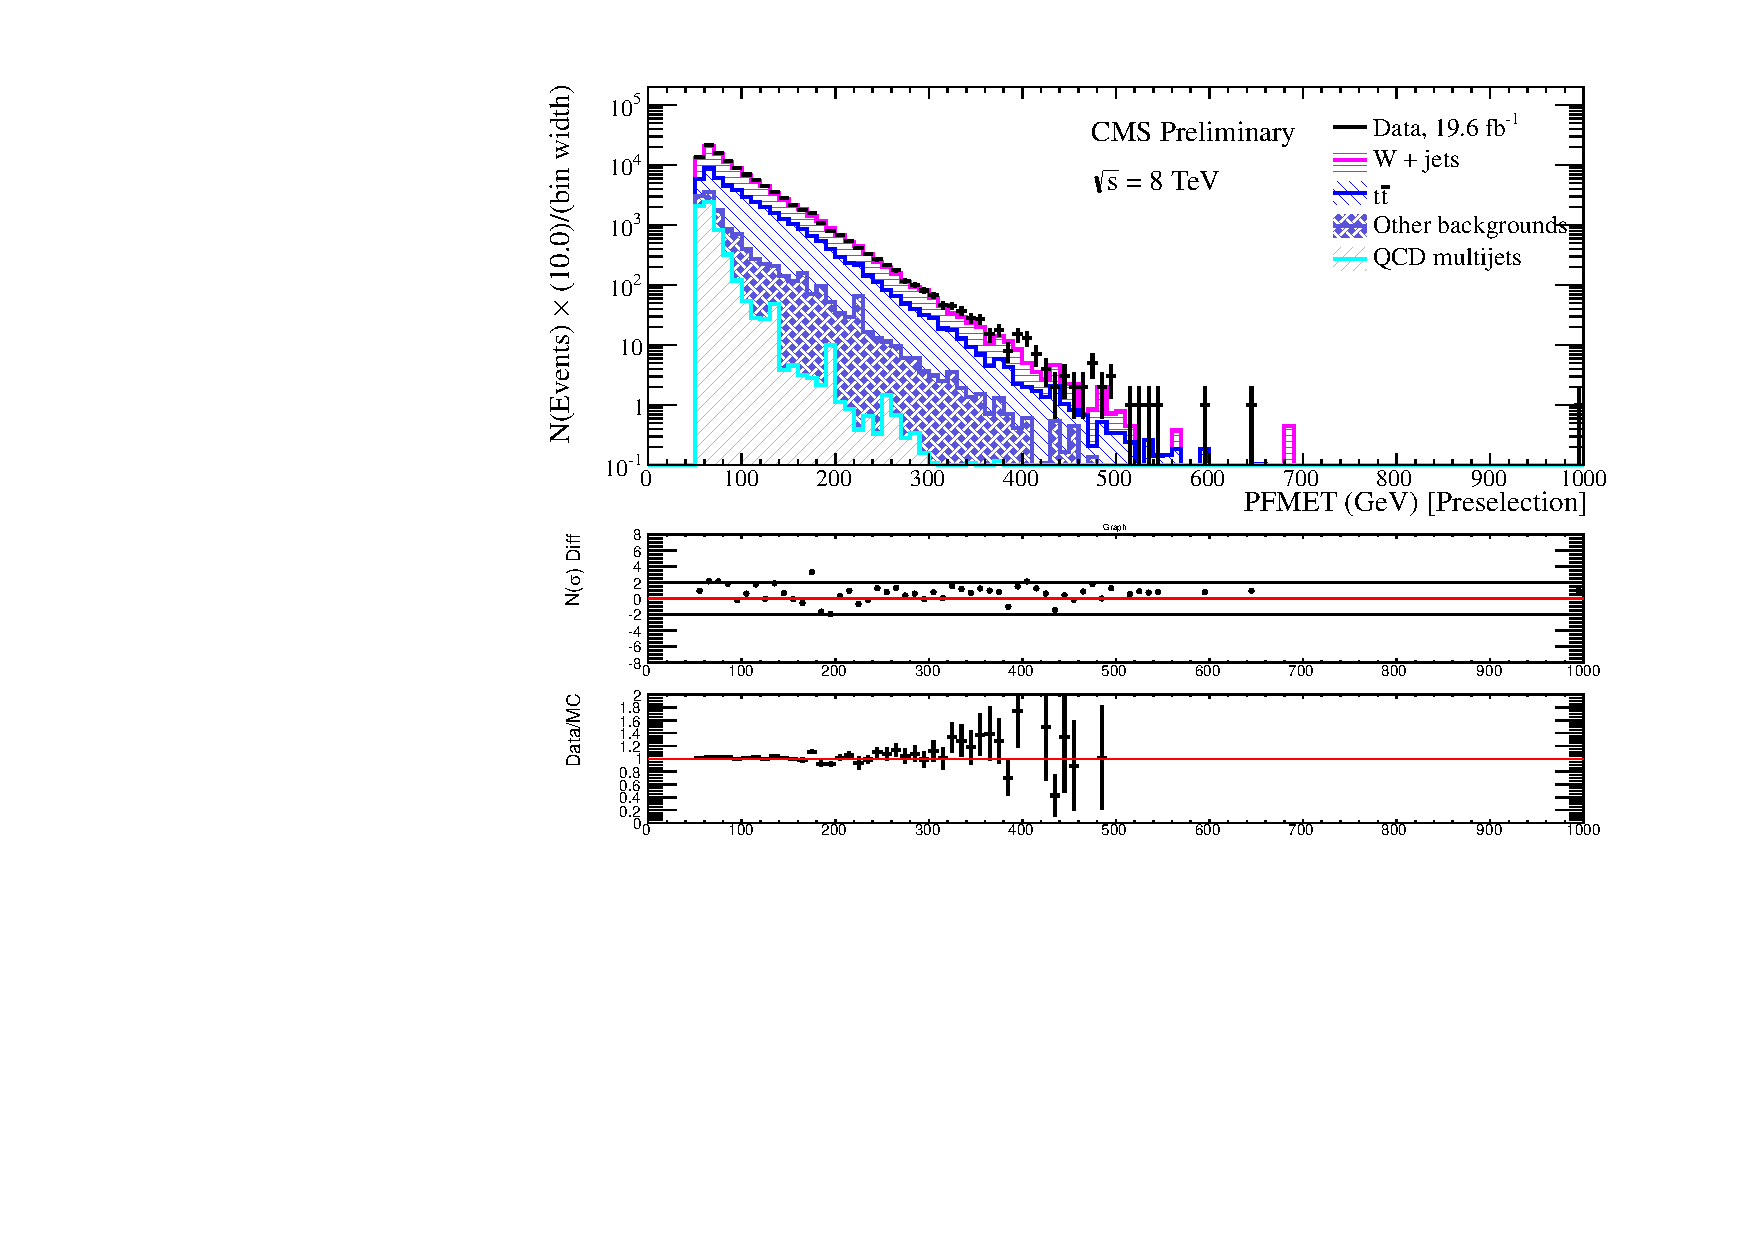
\includegraphics[width=\textwidth]{fig/enu/reweight/MET_PAS_enujjMETReweighted.pdf}
\end{column}
\begin{column}{0.6\textwidth}
%% \mt
\label{sec-1-9-5-1-2}

\centering
\mt after \met reweighting
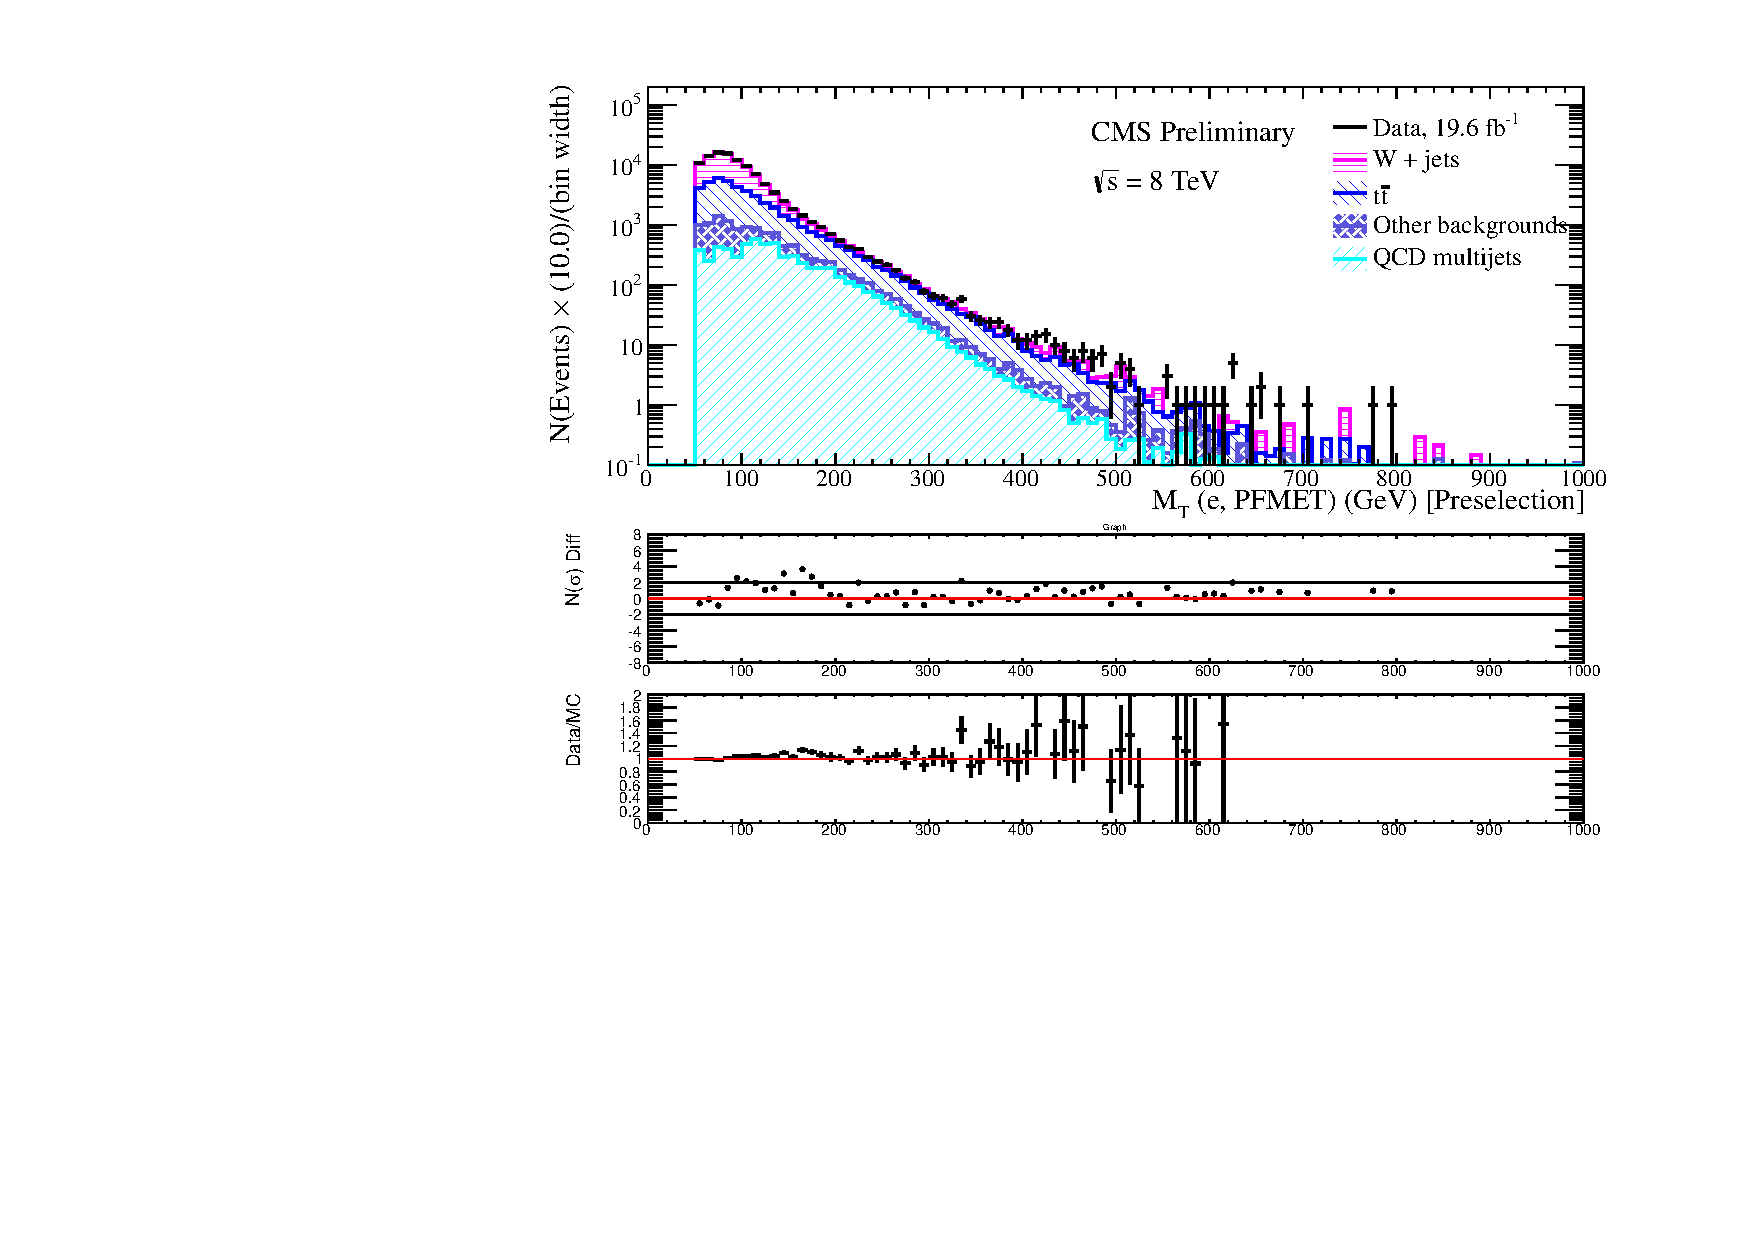
\includegraphics[width=\textwidth]{fig/enu/reweight/MTenu_PAS_enujjMETReweighted.pdf}
\end{column}
\end{columns}
%% Text
\label{sec-1-9-5-2}

\small
\centering
\met distribution improved, but \mt still needs help
\end{frame}
\begin{frame}
\frametitle{Find \mt function}
\label{sec-1-9-6}
\begin{columns} % Columns
\label{sec-1-9-6-1}
\begin{column}{0.6\textwidth}
%% \mt after \met reweighting
\label{sec-1-9-6-1-1}

\centering
\mt after \met reweighting
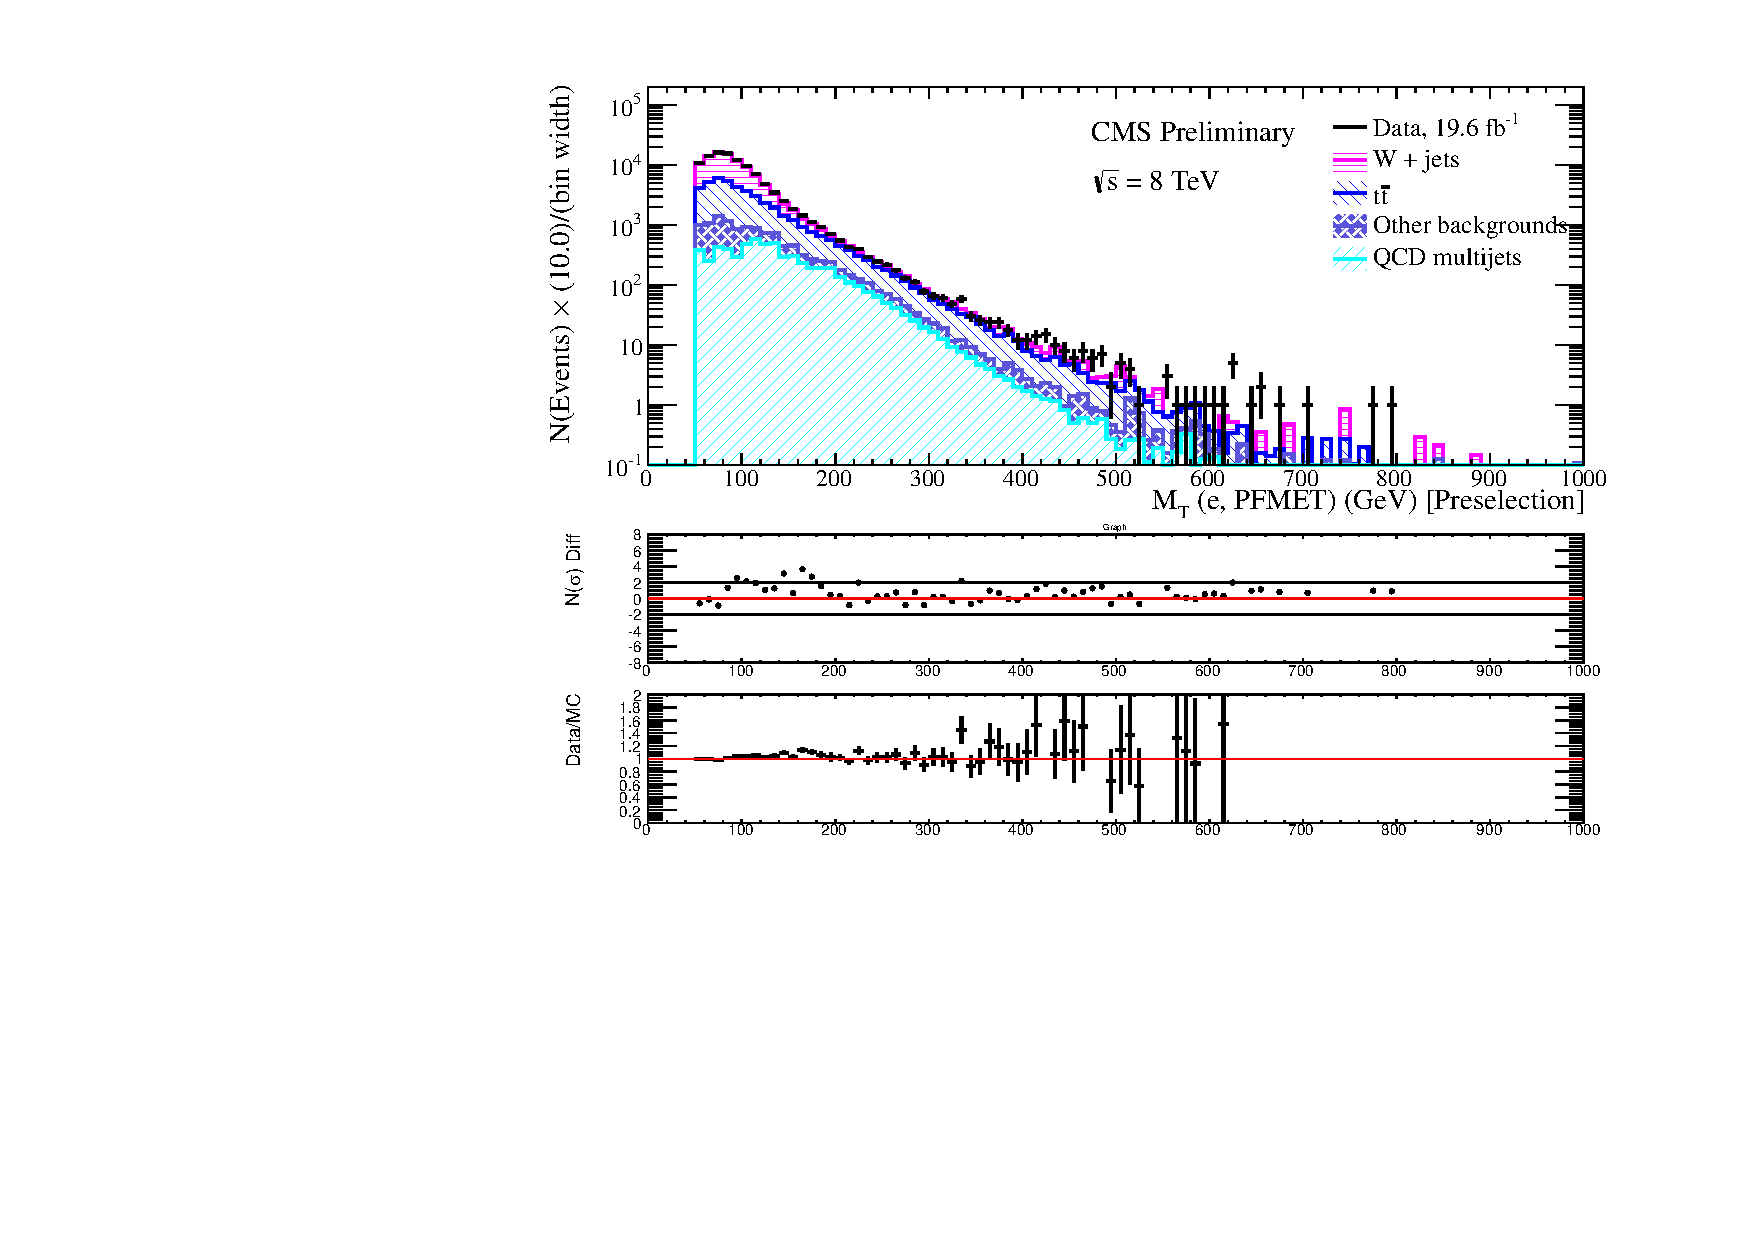
\includegraphics[width=\textwidth]{fig/enu/reweight/MTenu_PAS_enujjMETReweighted.pdf}
\end{column}
\begin{column}{0.6\textwidth}
%% Ratio
\label{sec-1-9-6-1-2}

\centering
\met reweighting function
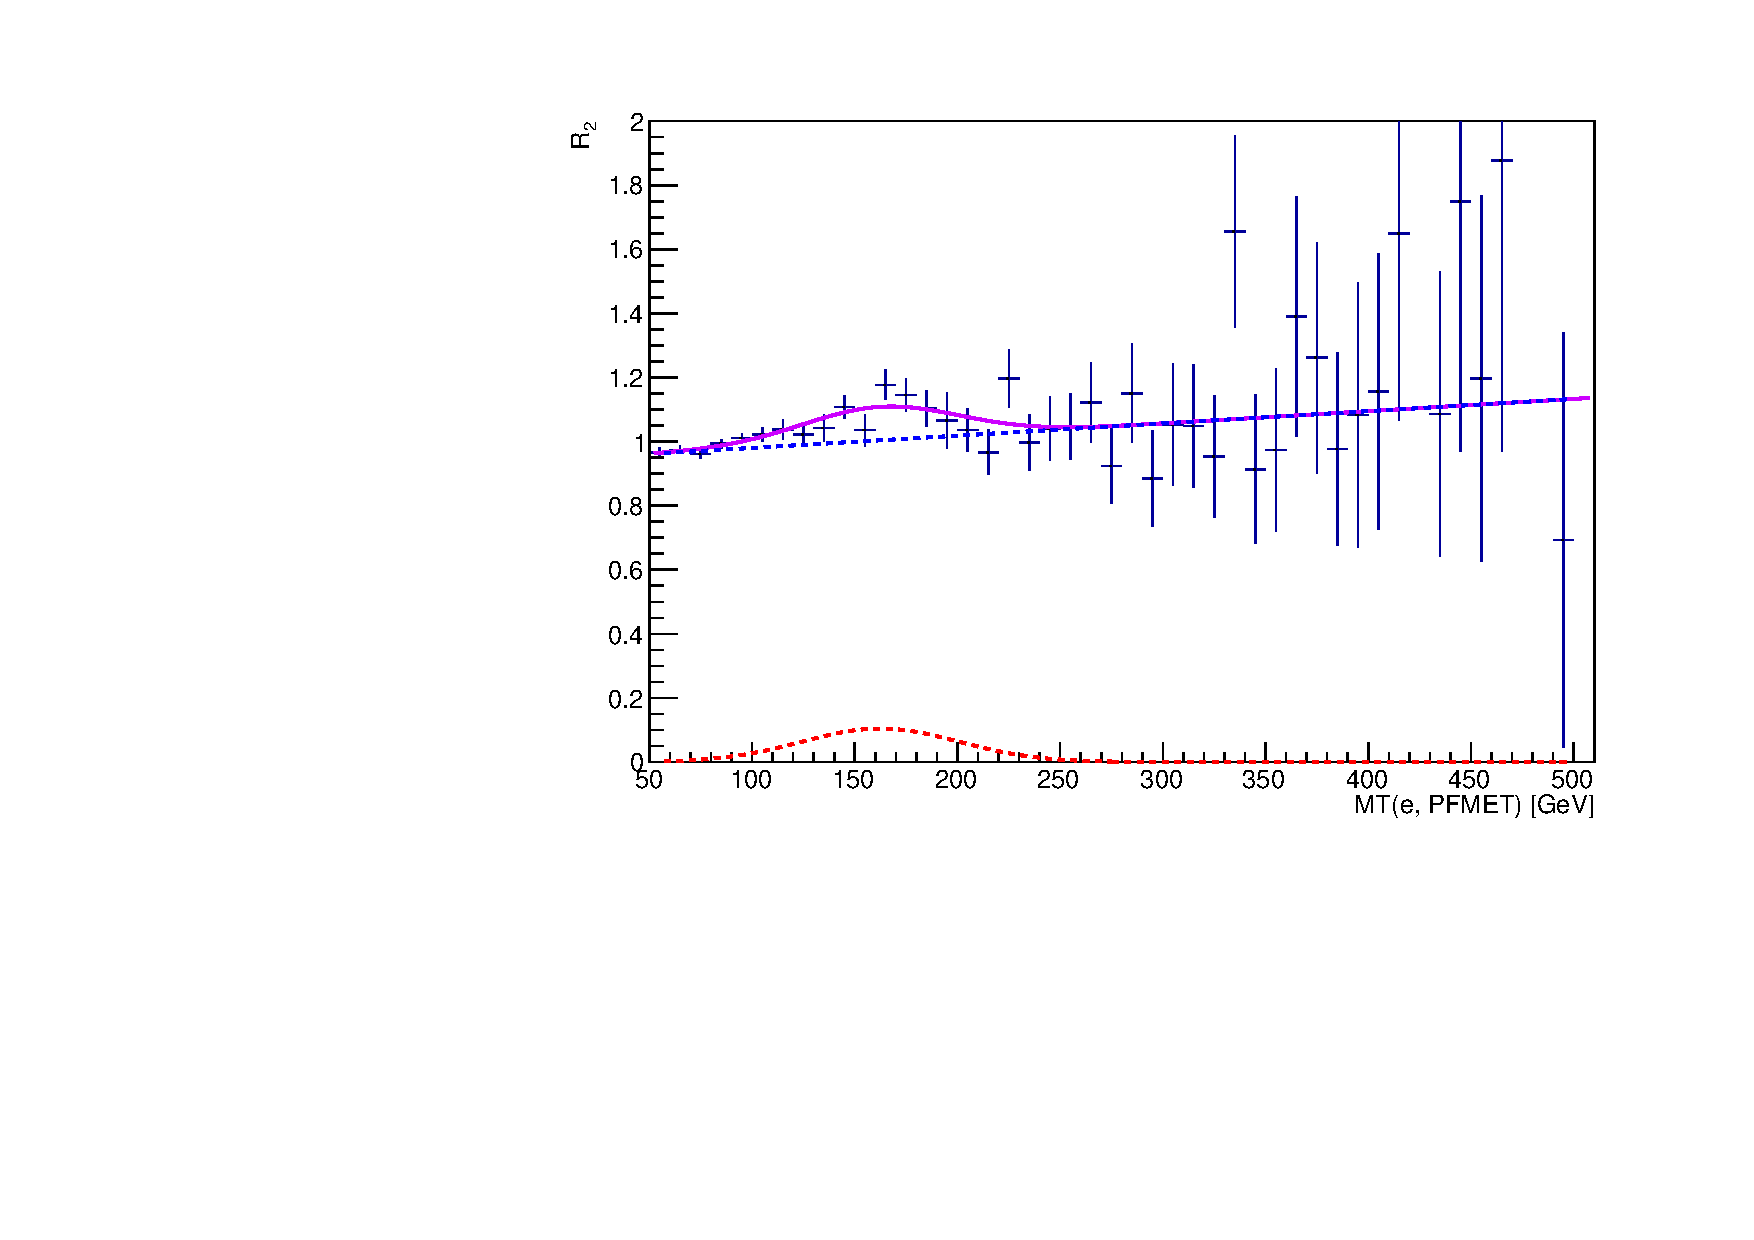
\includegraphics[width=\textwidth]{fig/enu/reweight/canvas_mt.pdf}
\end{column}
\end{columns}
%% Text
\label{sec-1-9-6-2}

\centering
\resizebox{!}{0.2\textheight}{\vbox{
Get reweighting function by fitting:
\begin{equation*}
  \mathcal{R}_2(\mt) = \frac{\text{N}_{i,\text{Data}}(\mt) - \text{N}_{i,\text{QCD}}(\mt)}{\text{N}_{i,\text{W}+\text{jets}}(\mt) + \text{N}_{i,\ttbar}(\mt) + \text{N}_{i,\text{Other}}(\mt)}
\end{equation*}
}}
\end{frame}
\begin{frame}
\frametitle{\mt function details}
\label{sec-1-9-7}
%% Text
\label{sec-1-9-7-1}

\centering
\begin{itemize}
\item Use the following linear fit function to define \mt reweighting:
\end{itemize}
\centering
\begin{equation*}
w_2(\mt) = b_{0} + b_{1}\cdot \mt + B \cdot e^{-\frac{1}{2}\cdot\left(\frac{\mt-\mu}{\sigma}\right)^2} 
\end{equation*}
\begin{itemize}
\item Fit returns the following parameters:
\end{itemize}
\resizebox*{!}{0.25\textheight}{
\begin{tabular}{|c|c|c|c|}
\hline
\hline
Parameter symbol & Parameter title & Mean value & Uncertainty \\
\hline
\hline
$b_0$    & Linear offset     & .942 & 0.0181 \\
$b_1$    & Linear slope      & $3.82 \cdot 10^{-4}$ & $1.68 \cdot 10^{-4}$ \\
\hline
$B$      & Gaussian constant & 0.104 & 0.0279 \\
$\mu$    & Gaussian width    & 38.2 & 11.6 \\
$\sigma$ & Gaussian mean     & 162 & 10.1 \\
\hline
\hline
\end{tabular}
}
\end{frame}
\begin{frame}
\frametitle{Rescale \wjets and \ttbar}
\label{sec-1-9-8}
%% Text
\label{sec-1-9-8-1}

\begin{itemize}
\item First apply $w_{\text{total}} = w_1(\met) \cdot w_2(\mt)$ to each MC event
\item Then rescale \wjets and \ttbar as before
\item Note: no \wjets and \ttbar rescaling applied so far
\end{itemize}
%% Equation
\label{sec-1-9-8-2}

\resizebox{\textwidth}{!}{
\begin{tabular}{ll}
$N^{1}_{\text{data}} = \mathcal{R}_{\ttbar} N_{\ttbar}^{1} + \mathcal{R}_{W} N_{W}^{1}  + N_{\text{QCD}}^{1} + N_{\text{Others}}^{1}$ &
$\mathcal{R}_{\ttbar} = \enujjTTBarMonteCarloScaleFactorMETandMTRescaled$ \\
$N^{2}_{\text{data}} = \mathcal{R}_{\ttbar} N_{\ttbar}^{2} + \mathcal{R}_{W} N_{W}^{2}  + N_{\text{QCD}}^{2} + N_{\text{Others}}^{2}$ &
$\mathcal{R}_{\text{W}} = \enujjWJetsMonteCarloScaleFactorMETandMTRescaled$ \\
\end{tabular}
}
\end{frame}
\begin{frame}
\frametitle{Apply \met and \mt reweights and rescale MC}
\label{sec-1-9-9}
\begin{columns} % Columns
\label{sec-1-9-9-1}
\begin{column}{0.6\textwidth}
%% \met
\label{sec-1-9-9-1-1}

\centering
\met after all reweighting
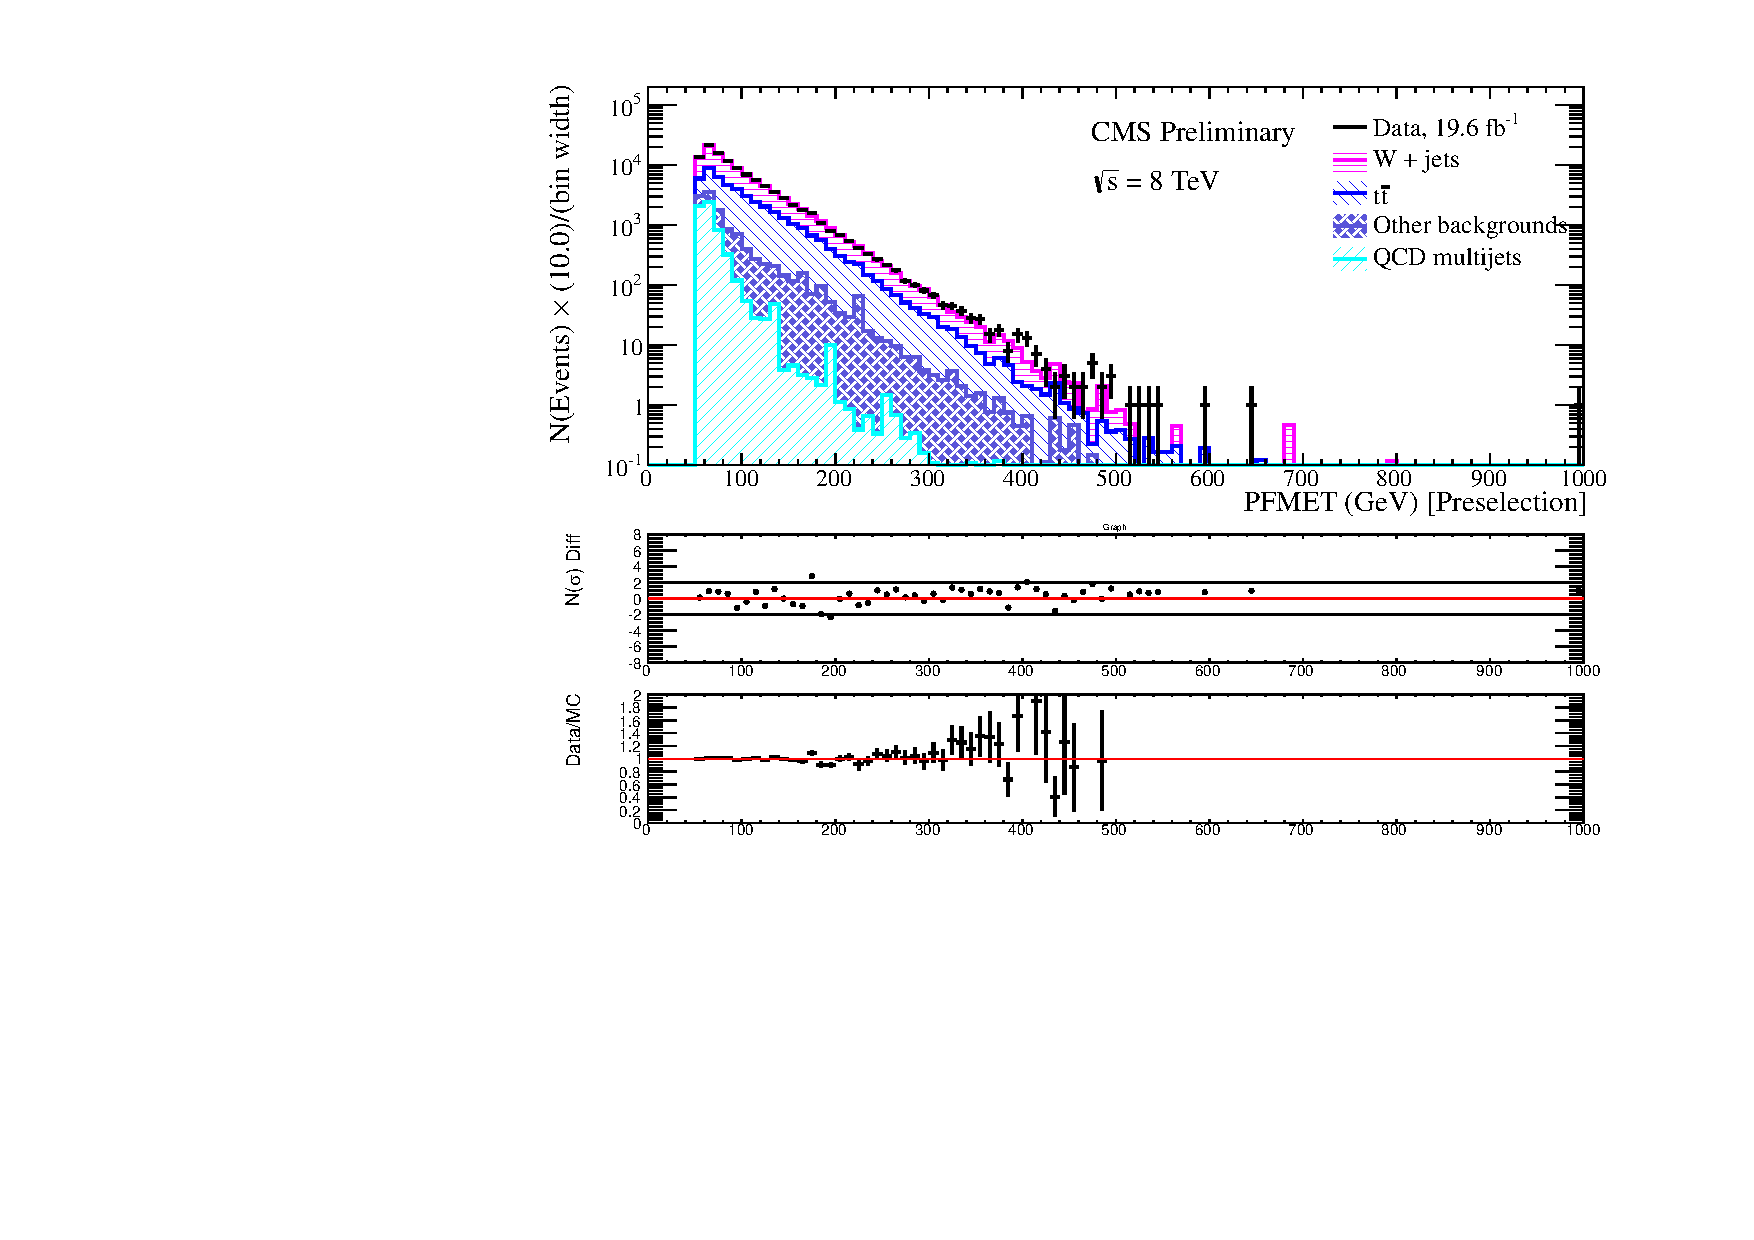
\includegraphics[width=\textwidth]{fig/enu/reweight/MET_PAS_enujjMETandMTReweighted.pdf}
\end{column}
\begin{column}{0.6\textwidth}
%% \mt
\label{sec-1-9-9-1-2}

\centering
\mt after all reweighting
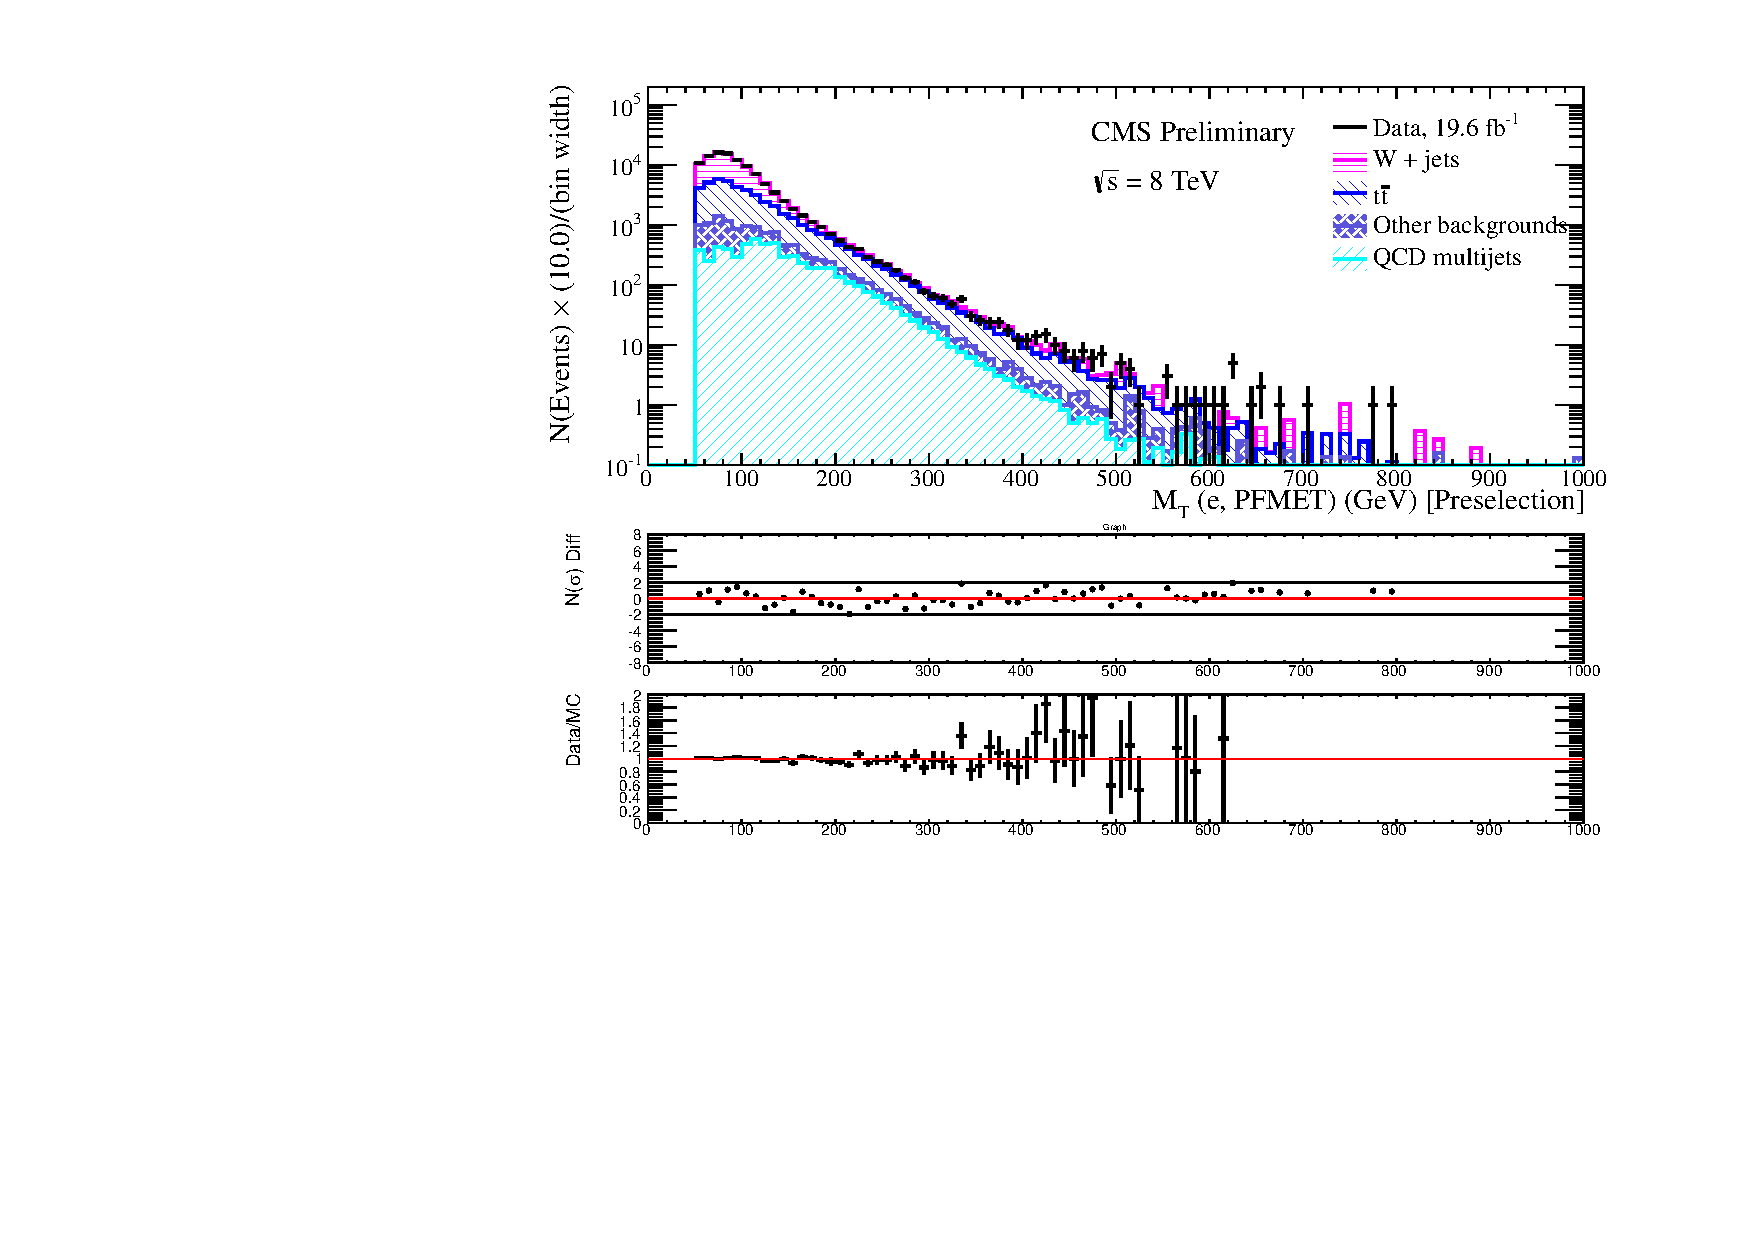
\includegraphics[width=\textwidth]{fig/enu/reweight/MTenu_PAS_enujjMETandMTReweighted.pdf}
\end{column}
\end{columns}
%% Text
\label{sec-1-9-9-2}

\small
\centering
Agreement much better in both \met and \mt distributions \\
after reweighting and rescaling
\end{frame}
\begin{frame}
\frametitle{\enujj final selection before reweighting}
\label{sec-1-9-10}
%% Table
\label{sec-1-9-10-1}

\centering
\resizebox{!}{0.6\textheight}{
\begin{tikzpicture}
\node (table) {
\begin{tabular}{| l | c | c | c | c | c | c | c |} 
\hline 
$M_{LQ} $ & LQ Signal & \wjets & \ttbar & QCD & Other & Data &  Total background \\ 
\hline 
\hline 
Presel & - &  $ 58284.8 \pm 197.0 $ & $ 32196.7 \pm 69.8 $ & $ 5950.5 \pm 20.1 $ & $ 6590.8 \pm 231.6 $ &105164 & $ 103022.8 \pm 312.6 $ \\ 
\hline 
300 &  $ 4765.5\pm 51.1 $ &  $ 822.1 \pm 22.4 $ & $ 1191.3 \pm 12.0 $ & $ 117.9 \pm 1.5 $ & $ 210.5 \pm 7.7 $ & 2455 &  $ 2341.90 \pm 26.58 $ $ \pm $ $ 163.90 $ (syst) \\ 
350 &  $ 2168.4\pm 21.6 $ &  $ 275.9 \pm 14.5 $ & $ 441.4 \pm 7.2 $ & $ 59.11 \pm 0.97 $ & $ 102.1 \pm 5.4 $ & 908 &  $ 878.55 \pm 17.08 $ $ \pm $ $ 58.66 $ (syst) \\ 
400 &  $ 971.1\pm 9.6 $ &  $ 110.4 \pm 7.8 $ & $ 184.2 \pm 4.7 $ & $ 32.88 \pm 0.69 $ & $ 51.5 \pm 3.8 $ & 413 &  $ 378.98 \pm 9.91 $ $ \pm $ $ 24.79 $ (syst) \\ 
450 &  $ 469.7\pm 4.6 $ &  $ 53.1 \pm 5.8 $ & $ 74.7 \pm 3.0 $ & $ 14.13 \pm 0.42 $ & $ 25.7 \pm 2.7 $ & 192 &  $ 167.64 \pm 7.06 $ $ \pm $ $ 11.01 $ (syst) \\ 
500 &  $ 232.7\pm 2.3 $ &  $ 20.5 \pm 3.3 $ & $ 34.4 \pm 2.0 $ & $ 7.76 \pm 0.30 $ & $ 15.3 \pm 2.1 $ & 83 &  $ 77.99 \pm 4.41 $ $ \pm $ $ 4.83 $ (syst) \\ 
550 &  $ 121.4\pm 1.2 $ &  $ 8.6 \pm 1.8 $ & $ 14.9 \pm 1.4 $ & $ 3.89 \pm 0.21 $ & $ 7.8 \pm 1.6 $ & 44 &  $ 35.24 \pm 2.76 $ $ \pm $ $ 2.18 $ (syst) \\ 
600 &  $ 66.37\pm 0.66 $ &  $ 2.3 \pm 1.0 $ & $ 7.08 \pm 0.93 $ & $ 2.29 \pm 0.17 $ & $ 4.6 \pm 1.2 $ & 28 &  $ 16.27 \pm 1.84 $ $ \pm $ $ 0.96 $ (syst) \\ 
650 &  $ 37.22\pm 0.37 $ &  $ 0.41 \pm 0.29 $ & $ 3.82 \pm 0.70 $ & $ 1.18 \pm 0.12 $ & $ 2.13 \pm 0.92 $ & 18 &  $ 7.54 \pm 1.20 $ $ \pm $ $ 0.52 $ (syst) \\ 
700 &  $ 21.74\pm 0.21 $ &  $ 0.41 \pm 0.29 $ & $ 2.61 \pm 0.60 $ & $ 0.85 \pm 0.10 $ & $ 0.58 \pm 0.24 $ & 6 &  $ 4.45 \pm 0.71 $ $ \pm $ $ 0.34 $ (syst) \\ 
750 &  $ 12.90\pm 0.13 $ &  $ 0.00_{-0.00}^{+0.94}$ &  $ 1.75 \pm 0.47 $ & $ 0.514 \pm 0.091 $ & $ 0.27 \pm 0.15 $ & 4 &  $ 2.535_{-0.504}^{+1.062}$ $ \pm $ $ 0.20 $ (syst)  \\ 
800 &  $ 7.610\pm 0.075 $ &  $ 0.00_{-0.00}^{+0.94}$ &  $ 1.10 \pm 0.37 $ & $ 0.317 \pm 0.067 $ & $ 0.27 \pm 0.15 $ & 3 &  $ 1.696_{-0.404}^{+1.019}$ $ \pm $ $ 0.13 $ (syst)  \\ 
850 &  $ 4.713\pm 0.046 $ &  $ 0.00_{-0.00}^{+0.94}$ &  $ 0.90 \pm 0.34 $ & $ 0.117 \pm 0.029 $ & $ 0.140 \pm 0.087 $ & 2 &  $ 1.153_{-0.353}^{+0.999}$ $ \pm $ $ 0.08 $ (syst)  \\ 
900 &  $ 2.929\pm 0.028 $ &  $ 0.00_{-0.00}^{+0.94}$ &  $ 0.37 \pm 0.21 $ & $ 0.076 \pm 0.024 $ & $ 0.084 \pm 0.069 $ & 1 &  $ 0.530_{-0.226}^{+0.962}$ $ \pm $ $ 0.04 $ (syst)  \\ 
950 &  $ 1.839\pm 0.018 $ &  $ 0.00_{-0.00}^{+0.94}$ &  $ 0.37 \pm 0.21 $ & $ 0.069 \pm 0.023 $ & $ 0.084 \pm 0.069 $ & 1 &  $ 0.524_{-0.226}^{+0.962}$ $ \pm $ $ 0.04 $ (syst)  \\ 
1000 &  $ 1.306\pm 0.012 $ &  $ 0.00_{-0.00}^{+0.94}$ &  $ 0.37 \pm 0.21 $ & $ 0.069 \pm 0.023 $ & $ 0.084 \pm 0.069 $ & 1 &  $ 0.524_{-0.226}^{+0.962}$ $ \pm $ $ 0.04 $ (syst)  \\ 
1050 &  $ 0.9022\pm 0.0076 $ &  $ 0.00_{-0.00}^{+0.94}$ &  $ 0.37 \pm 0.21 $ & $ 0.069 \pm 0.023 $ & $ 0.084 \pm 0.069 $ & 1 &  $ 0.524_{-0.226}^{+0.962}$ $ \pm $ $ 0.04 $ (syst)  \\ 
1100 &  $ 0.6225\pm 0.0050 $ &  $ 0.00_{-0.00}^{+0.94}$ &  $ 0.37 \pm 0.21 $ & $ 0.069 \pm 0.023 $ & $ 0.084 \pm 0.069 $ & 1 &  $ 0.524_{-0.226}^{+0.962}$ $ \pm $ $ 0.04 $ (syst)  \\ 
1150 &  $ 0.4308\pm 0.0032 $ &  $ 0.00_{-0.00}^{+0.94}$ &  $ 0.37 \pm 0.21 $ & $ 0.069 \pm 0.023 $ & $ 0.084 \pm 0.069 $ & 1 &  $ 0.524_{-0.226}^{+0.962}$ $ \pm $ $ 0.04 $ (syst)  \\ 
1200 &  $ 0.2971\pm 0.0022 $ &  $ 0.00_{-0.00}^{+0.94}$ &  $ 0.37 \pm 0.21 $ & $ 0.069 \pm 0.023 $ & $ 0.084 \pm 0.069 $ & 1 &  $ 0.524_{-0.226}^{+0.962}$ $ \pm $ $ 0.04 $ (syst)  \\ 
\hline 
\end{tabular}
};
\draw [red,ultra thick,rounded corners]
($(table.south west) !.52! (table.north west)$)
rectangle 
($(table.south east) !.57! (table.north east)$);    
\draw [red,ultra thick,rounded corners]
($(table.north east) !.322! (table.north west)$)
rectangle 
($(table.south east) !0.! (table.north west)$);    
\end{tikzpicture}
}%
\end{frame}
\begin{frame}
\frametitle{\enujj final selection after reweighting}
\label{sec-1-9-11}
%% Table
\label{sec-1-9-11-1}

\centering
\resizebox*{!}{0.6\textheight}{
\begin{tikzpicture}
\node (table) {
\begin{tabular}{| l | c | c | c | c | c | c |} 
  \hline 
$M_{LQ}$ & W+Jets & $t\bar{t}$ & QCD & Other & Data &  Total BG \\ 
  \hline 
  \hline 
Presel &  $ 59725.3 \pm 201.9 $ & $ 33176.5 \pm 71.7 $ & $ 5950.5 \pm 20.1 $ & $ 5943.8 \pm 205.5 $ &105164 & $ 104796.0 \pm 297.6 $ \\ 
  \hline 
300 &  $ 859.6 \pm 23.1 $ & $ 1233.0 \pm 12.4 $ & $ 117.9 \pm 1.5 $ & $ 187.6 \pm 6.907 $ &2455 & $ 2398.04 \pm 27.16 $ \\ 
350 &  $ 280.4 \pm 14.4 $ & $ 446.3 \pm 7.3 $ & $ 59.11 \pm 0.97 $ & $ 88.6 \pm 4.649 $ &908 & $ 874.28 \pm 16.83 $ \\ 
400 &  $ 108.5 \pm 7.7 $ & $ 180.6 \pm 4.6 $ & $ 32.88 \pm 0.69 $ & $ 43.7 \pm 3.229 $ &413 & $ 365.71 \pm 9.55 $ \\ 
450 &  $ 50.5 \pm 5.5 $ & $ 70.8 \pm 2.8 $ & $ 14.13 \pm 0.42 $ & $ 21.3 \pm 2.257 $ &192 & $ 156.75 \pm 6.62 $ \\ 
500 &  $ 19.0 \pm 3.0 $ & $ 31.6 \pm 1.9 $ & $ 7.76 \pm 0.30 $ & $ 12.4 \pm 1.734 $ &83 & $ 70.81 \pm 3.93 $ \\ 
550 &  $ 7.9 \pm 1.7 $ & $ 13.3 \pm 1.2 $ & $ 3.89 \pm 0.21 $ & $ 6.3 \pm 1.288 $ &44 & $ 31.36 \pm 2.43 $ \\ 
600 &  $ 2.2 \pm 0.9 $ & $ 6.13 \pm 0.80 $ & $ 2.29 \pm 0.17 $ & $ 3.5 \pm 0.959 $ &28 & $ 14.08 \pm 1.57 $ \\ 
650 &  $ 0.43 \pm 0.30 $ & $ 3.22 \pm 0.59 $ & $ 1.18 \pm 0.12 $ & $ 1.59 \pm 0.736 $ &18 & $ 6.43 \pm 1.00 $ \\ 
700 &  $ 0.43 \pm 0.30 $ & $ 2.17 \pm 0.50 $ & $ 0.85 \pm 0.10 $ & $ 0.35 \pm 0.150 $ &6 & $ 3.80 \pm 0.61 $ \\ 
750 &  $ 0.00_{-0.00}^{+0.94}$ &  $ 1.49 \pm 0.41 $ & $ 0.514 \pm 0.091 $ & $ 0.117 \pm 0.061 $ &4 & $ 2.116_{-0.420}^{+1.025}$ \\ 
800 &  $ 0.00_{-0.00}^{+0.94}$ &  $ 0.87 \pm 0.30 $ & $ 0.317 \pm 0.067 $ & $ 0.116 \pm 0.061 $ &3 & $ 1.308_{-0.313}^{+0.986}$ \\ 
850 &  $ 0.00_{-0.00}^{+0.94}$ &  $ 0.70 \pm 0.27 $ & $ 0.117 \pm 0.029 $ & $ 0.054 \pm 0.032 $ &2 & $ 0.874_{-0.278}^{+0.975}$ \\ 
900 &  $ 0.00_{-0.00}^{+0.94}$ &  $ 0.27 \pm 0.16 $ & $ 0.076 \pm 0.024 $ & $ 0.019 \pm 0.012 $ &1 & $ 0.366_{-0.159}^{+0.948}$ \\ 
950 &  $ 0.00_{-0.00}^{+0.94}$ &  $ 0.27 \pm 0.16 $ & $ 0.069 \pm 0.023 $ & $ 0.019 \pm 0.012 $ &1 & $ 0.359_{-0.159}^{+0.948}$ \\ 
1000 &  $ 0.00_{-0.00}^{+0.94}$ &  $ 0.27 \pm 0.16 $ & $ 0.069 \pm 0.023 $ & $ 0.019 \pm 0.012 $ &1 & $ 0.359_{-0.159}^{+0.948}$ \\ 
1050 &  $ 0.00_{-0.00}^{+0.94}$ &  $ 0.27 \pm 0.16 $ & $ 0.069 \pm 0.023 $ & $ 0.019 \pm 0.012 $ &1 & $ 0.359_{-0.159}^{+0.948}$ \\ 
1100 &  $ 0.00_{-0.00}^{+0.94}$ &  $ 0.27 \pm 0.16 $ & $ 0.069 \pm 0.023 $ & $ 0.019 \pm 0.012 $ &1 & $ 0.359_{-0.159}^{+0.948}$ \\ 
1150 &  $ 0.00_{-0.00}^{+0.94}$ &  $ 0.27 \pm 0.16 $ & $ 0.069 \pm 0.023 $ & $ 0.019 \pm 0.012 $ &1 & $ 0.359_{-0.159}^{+0.948}$ \\ 
1200 &  $ 0.00_{-0.00}^{+0.94}$ &  $ 0.27 \pm 0.16 $ & $ 0.069 \pm 0.023 $ & $ 0.019 \pm 0.012 $ &1 & $ 0.359_{-0.159}^{+0.948}$ \\ 
  \hline 
\end{tabular}
};
\draw [red,ultra thick,rounded corners]
($(table.south west) !.525! (table.north west)$)
rectangle 
($(table.south east) !.575! (table.north east)$);    
\draw [red,ultra thick,rounded corners]
($(table.north east) !.283! (table.north west)$)
rectangle 
($(table.south east) !0.! (table.north west)$);  
\end{tikzpicture}
}%
%% Text
\label{sec-1-9-11-2}

\begin{itemize}
\item Discrepancy at 650 selection increases after reweighting
\item No change made to the analysis
\end{itemize}
\end{frame}
\subsection{\eejj extra plots}
\label{sec-1-10}
\begin{frame}
\frametitle{\eejj extra plots}
\label{sec-1-10-1}
\begin{columns} % Columns
\label{sec-1-10-1-1}
\begin{column}{0.475\textwidth}
%% 1st column
\label{sec-1-10-1-1-1}
%% 1st block in 1st column
\label{sec-1-10-1-1-2}

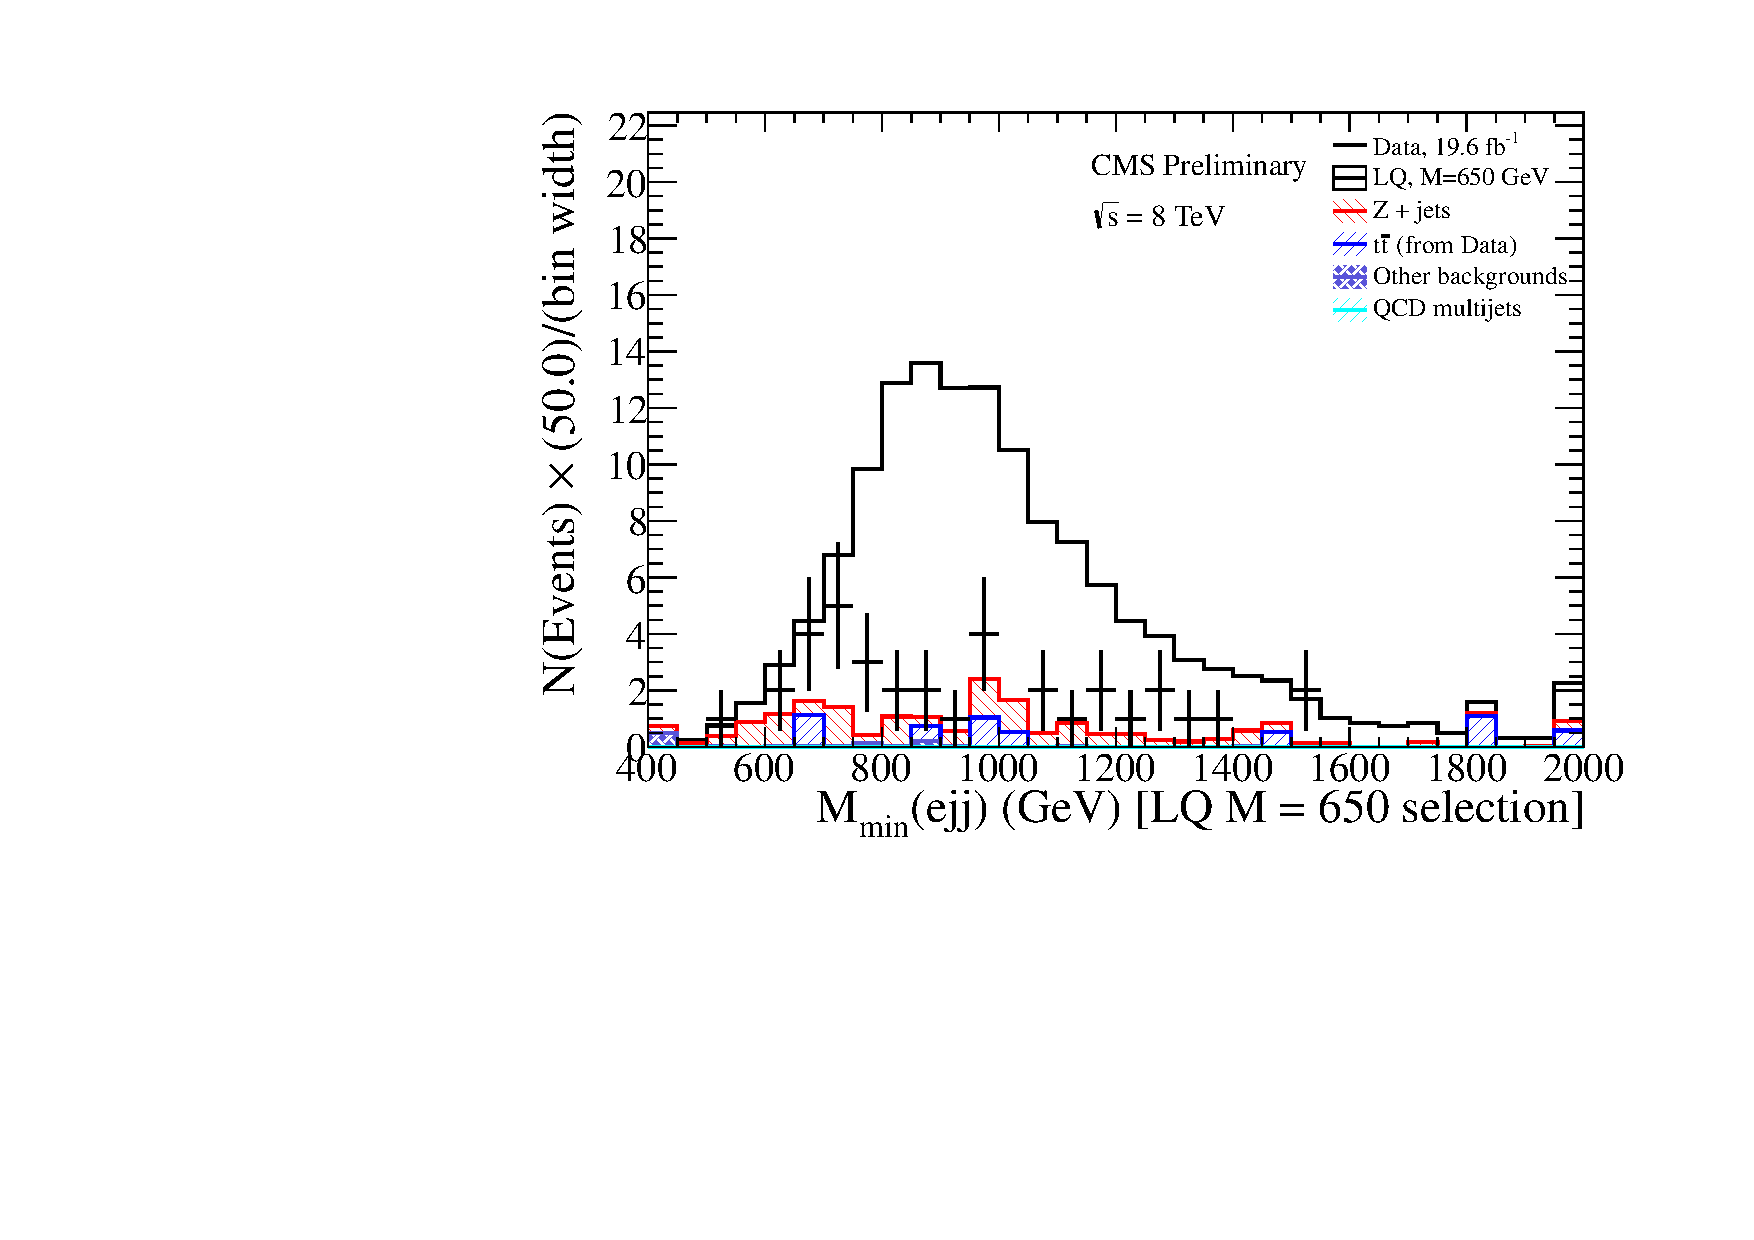
\includegraphics[width=0.8\textwidth]{fig/ee/extra/MejjMin_LQ650_eejj.pdf}
%% 2nd block in 1st column
\label{sec-1-10-1-1-3}

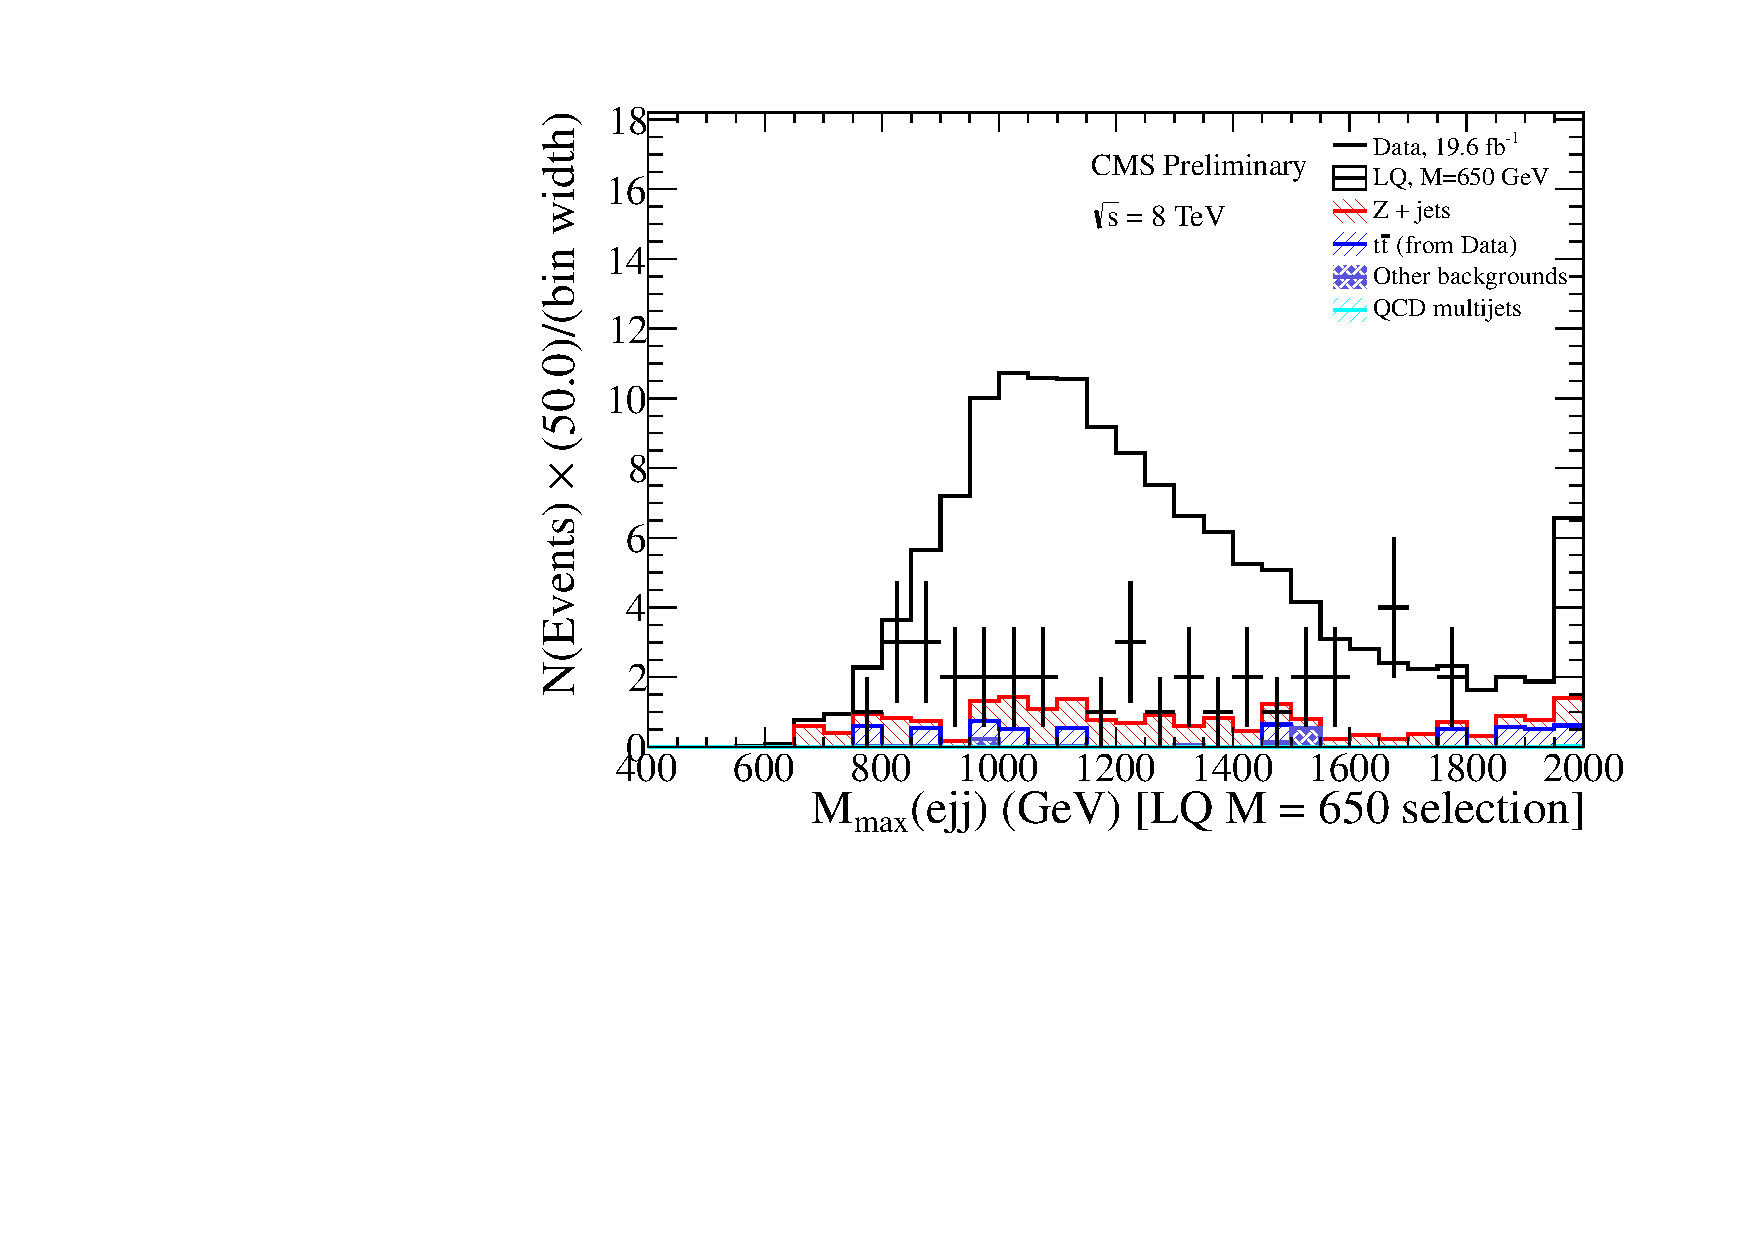
\includegraphics[width=0.8\textwidth]{fig/ee/extra/MejjMax_LQ650_eejj.pdf}
\end{column}
\begin{column}{0.475\textwidth}
%% 2nd column
\label{sec-1-10-1-1-4}
%% 1st block in 2nd column
\label{sec-1-10-1-1-5}

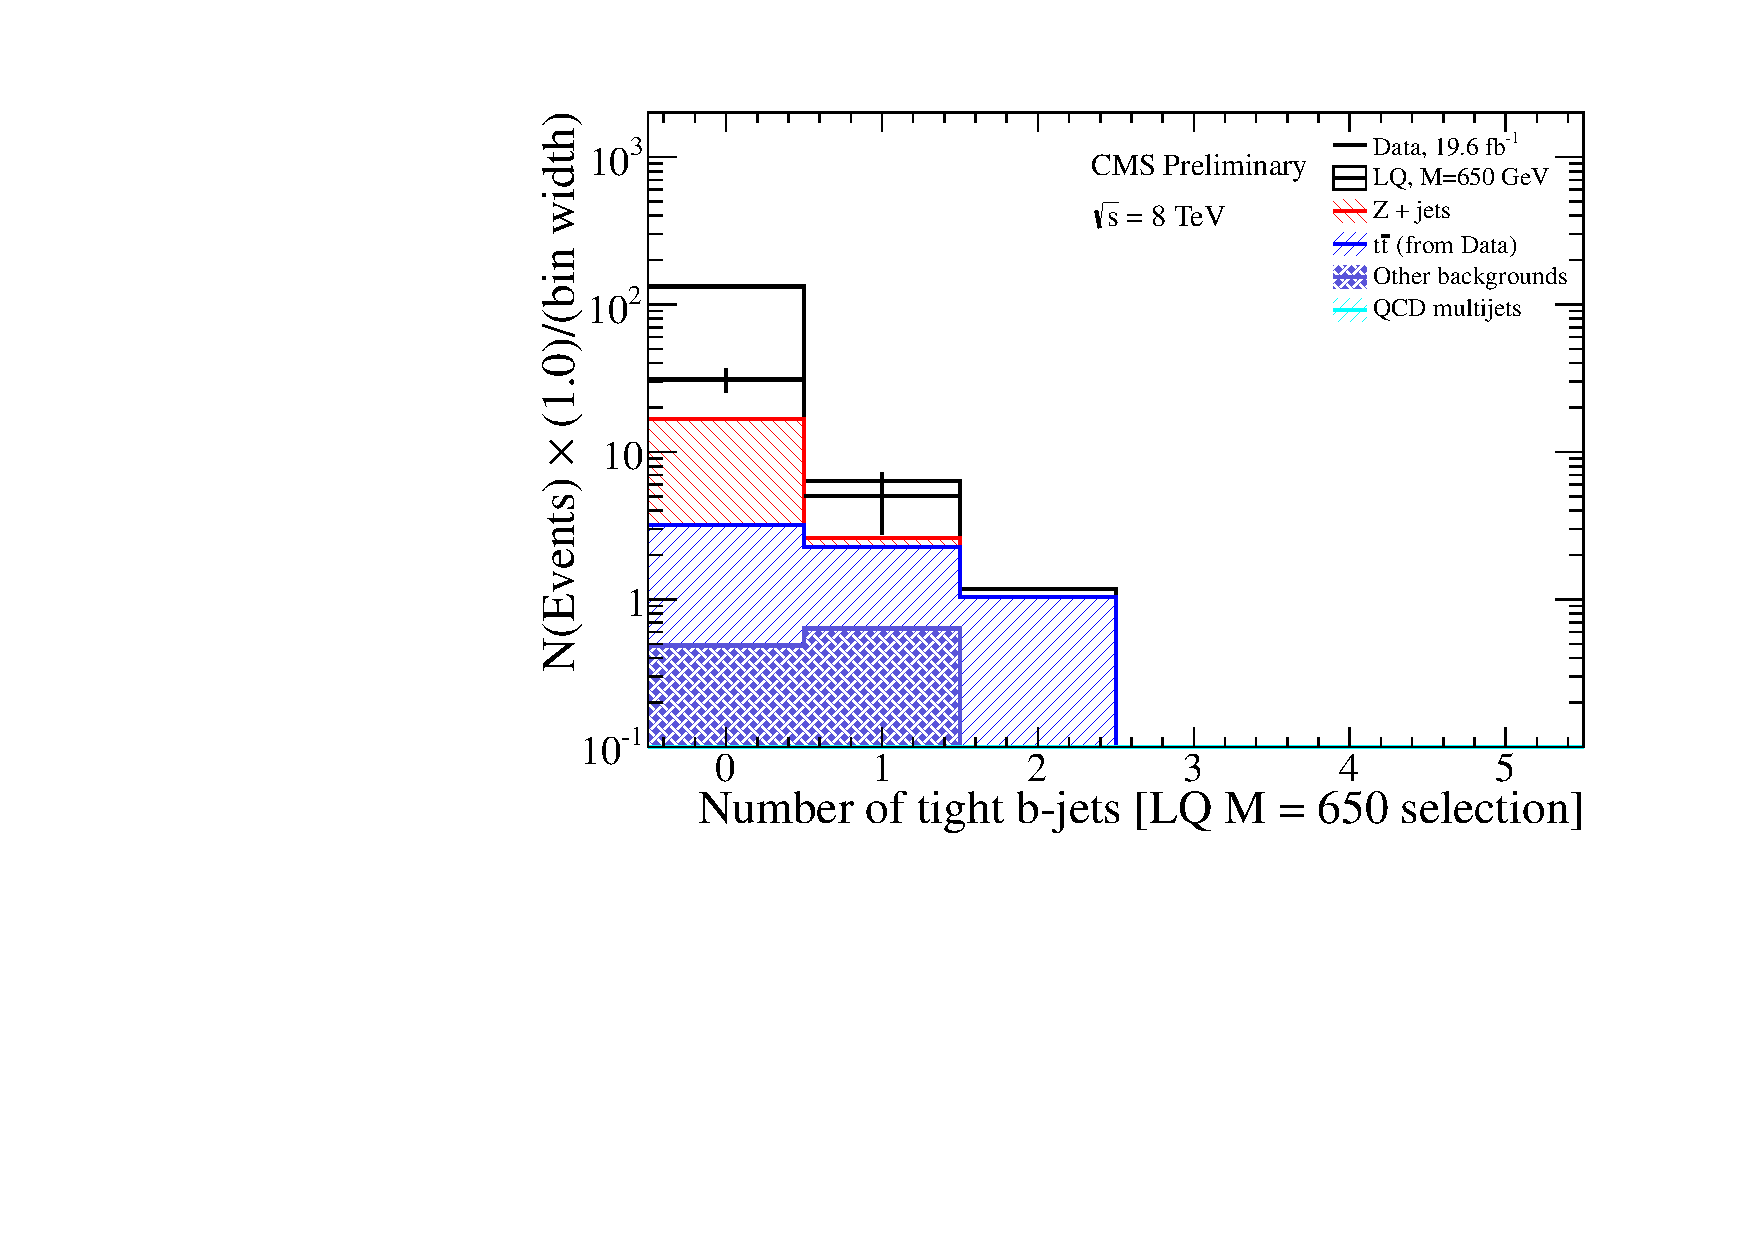
\includegraphics[width=0.8\textwidth]{fig/ee/extra/nBJet_tight_LQ650_eejj.pdf}
%% 2nd block in the 2nd column
\label{sec-1-10-1-1-6}

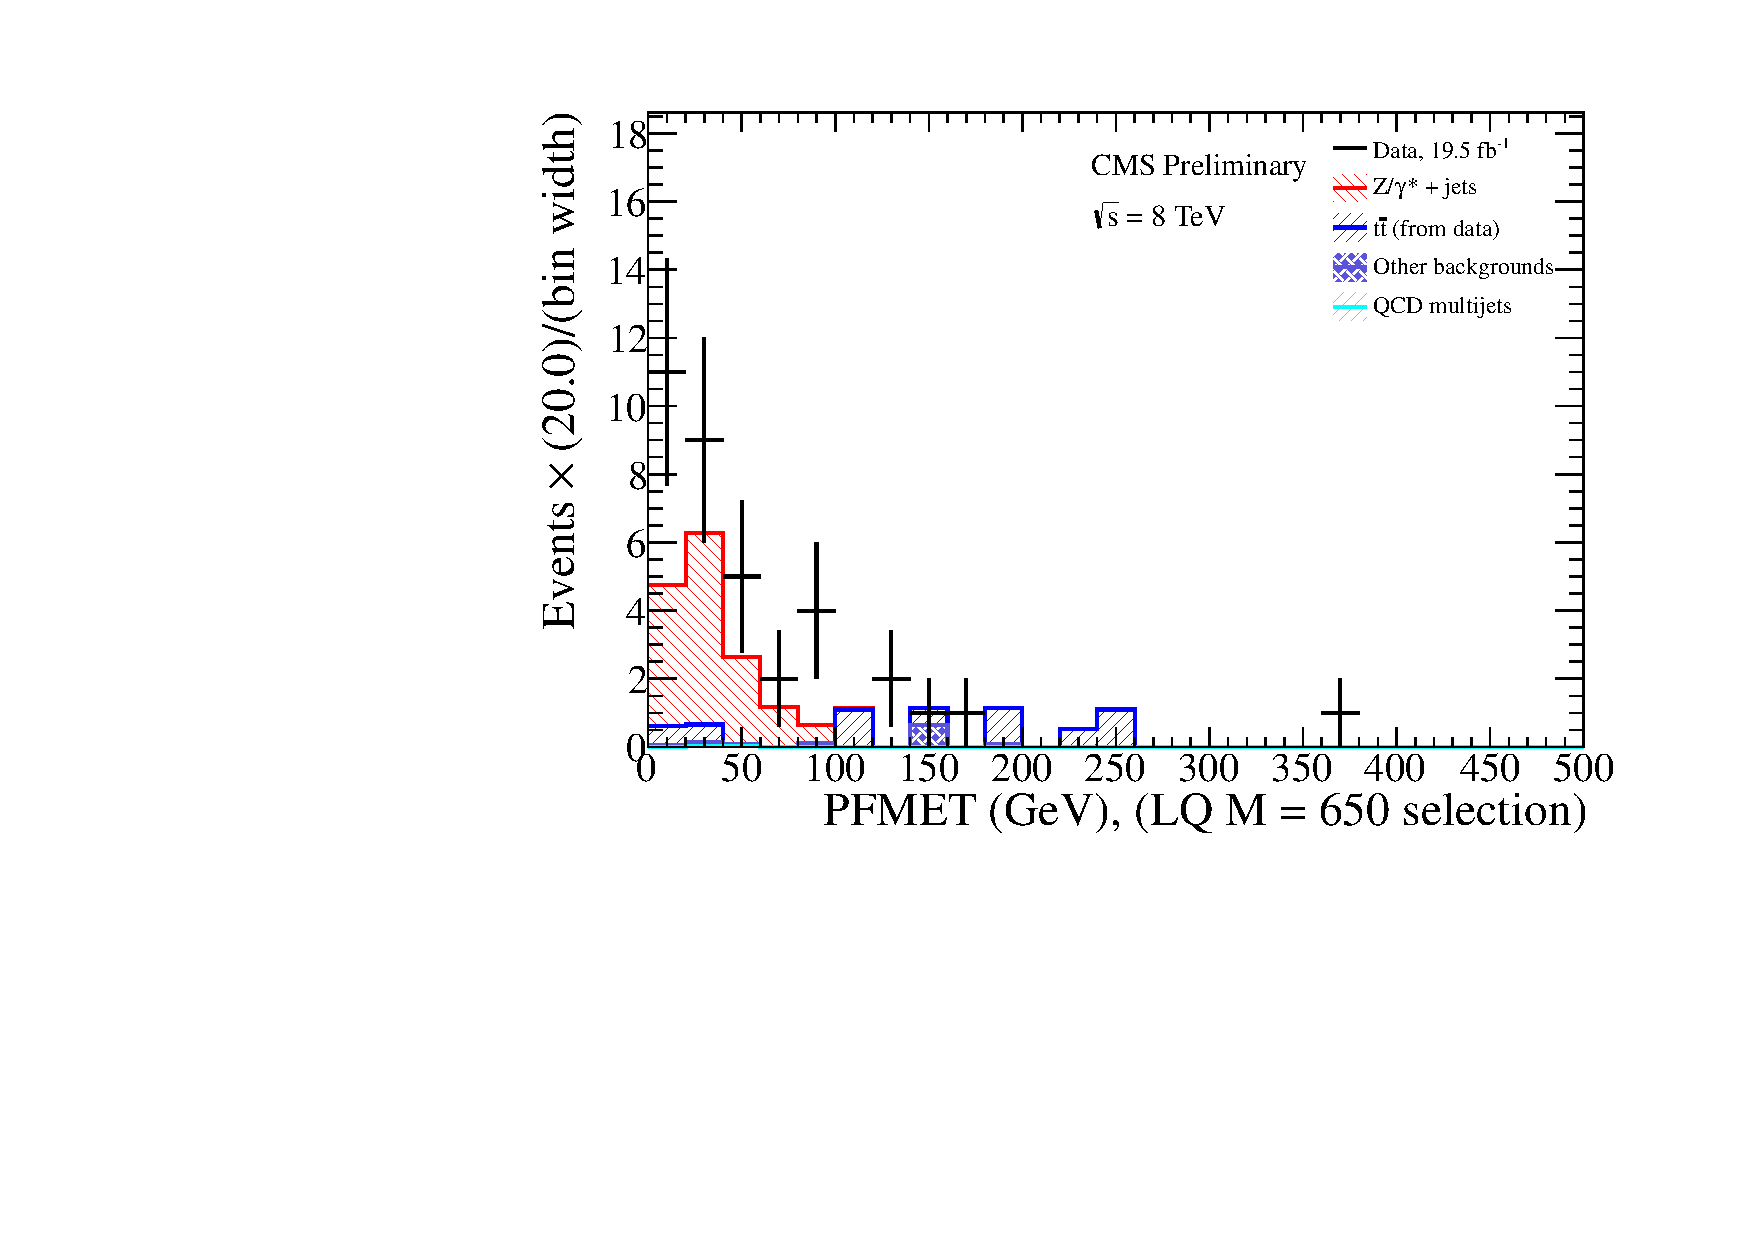
\includegraphics[width=0.8\textwidth]{fig/ee/extra/MET_LQ650_eejj_finalOnly.pdf}
\end{column}
\end{columns}
\end{frame}
\subsection{\enujj extra plots}
\label{sec-1-11}
\begin{frame}
\frametitle{\enujj extra plots}
\label{sec-1-11-1}
\begin{columns} % Columns
\label{sec-1-11-1-1}
\begin{column}{0.475\textwidth}
%% 1st column
\label{sec-1-11-1-1-1}
%% 1st block in 1st column
\label{sec-1-11-1-1-2}

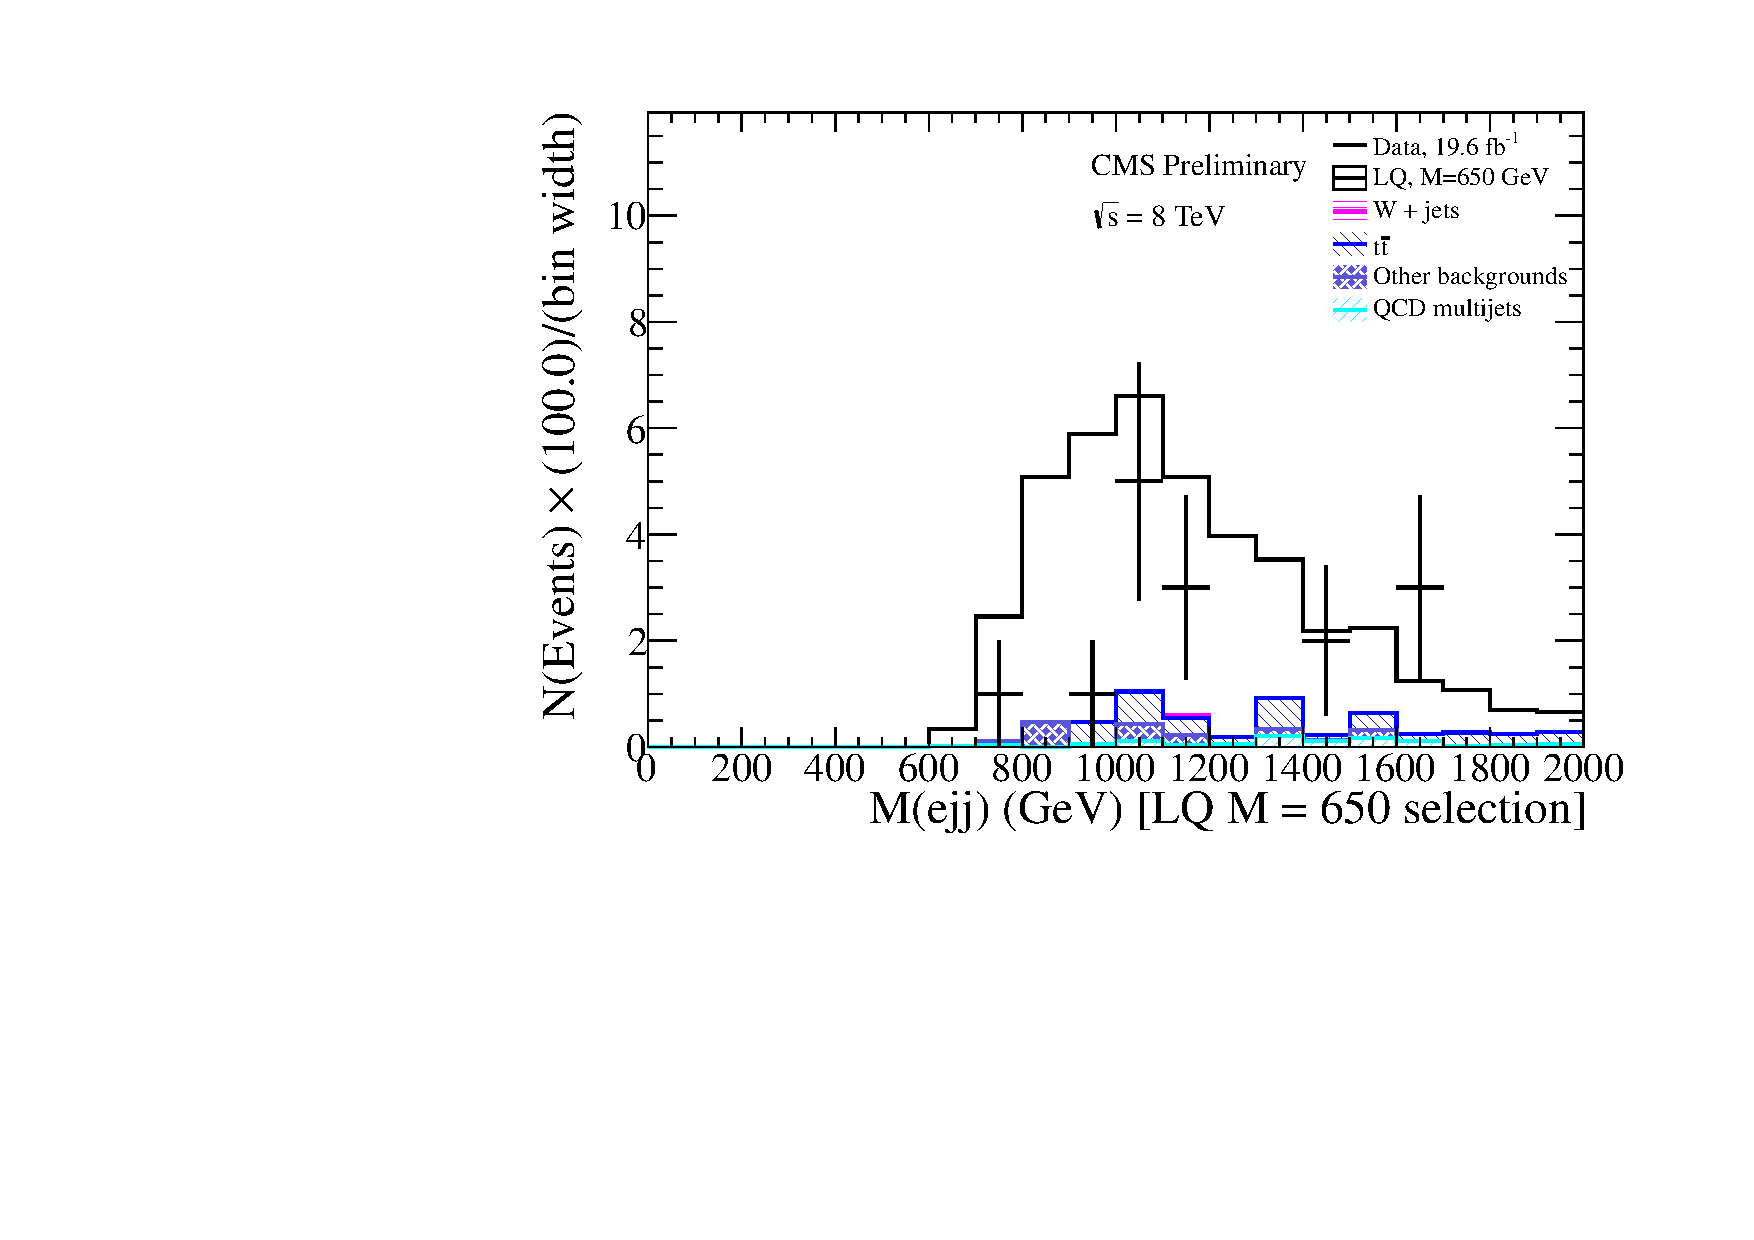
\includegraphics[width=0.8\textwidth]{fig/enu/extra/Mejj_LQ650_enujj.pdf}
%% 2nd block in 1st column
\label{sec-1-11-1-1-3}

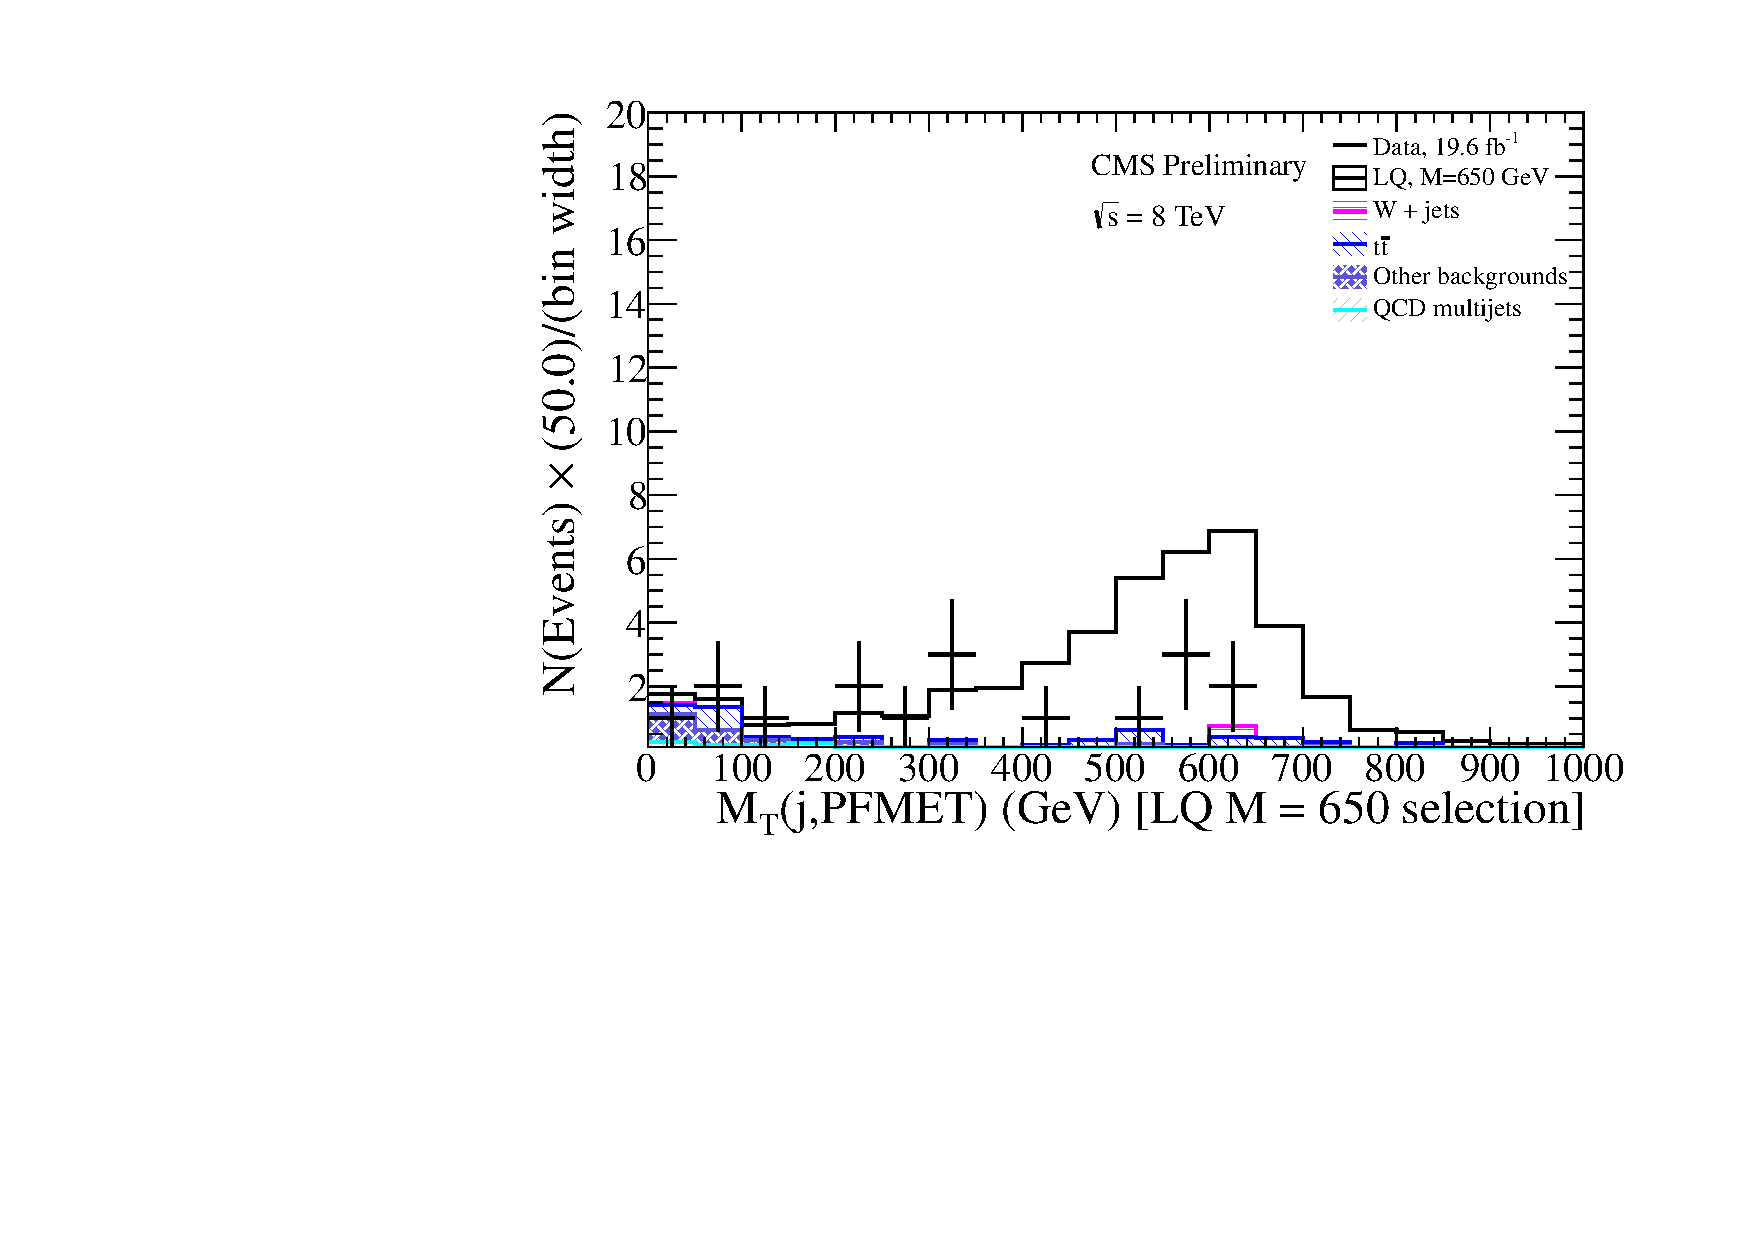
\includegraphics[width=0.8\textwidth]{fig/enu/extra/MTjnu_LQ650_enujj.pdf}
\end{column}
\begin{column}{0.475\textwidth}
%% 2nd column
\label{sec-1-11-1-1-4}
%% 1st block in 2nd column
\label{sec-1-11-1-1-5}

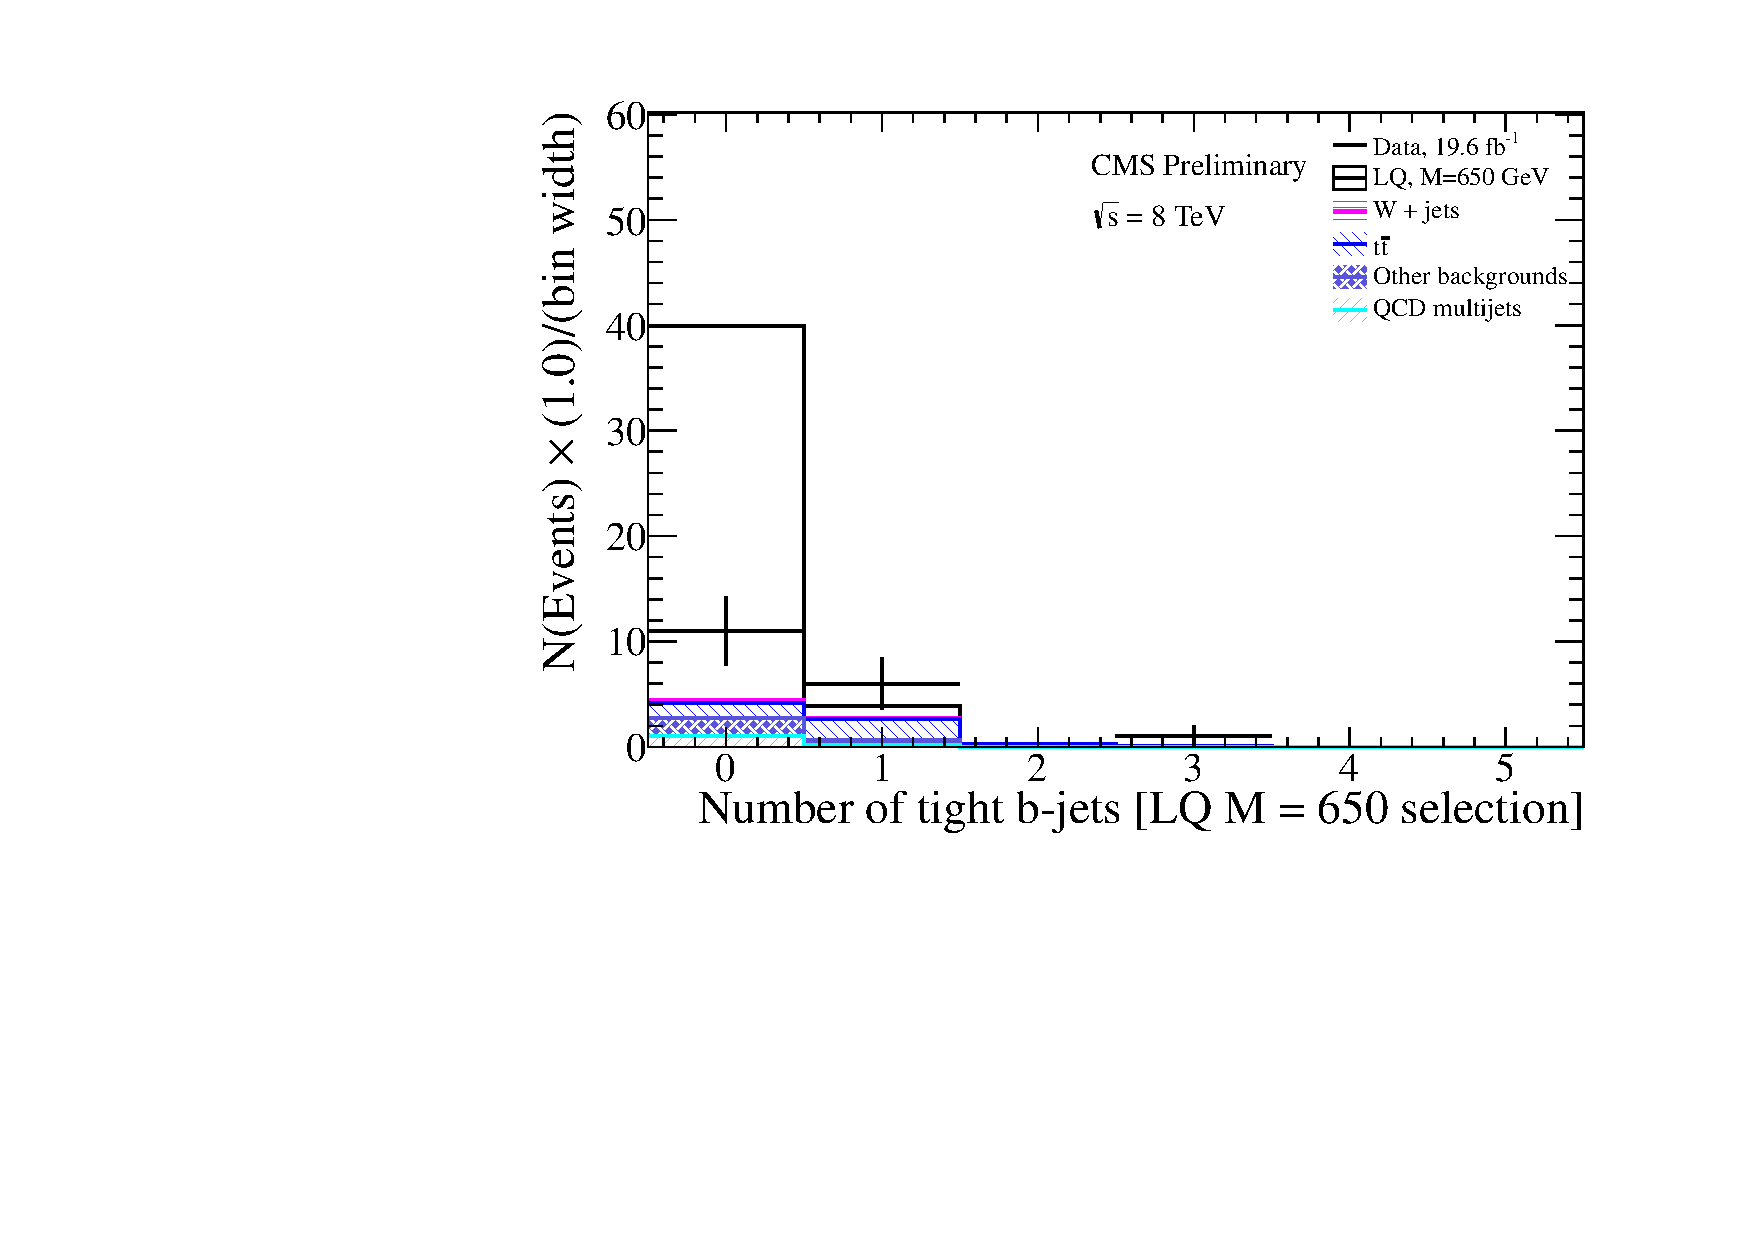
\includegraphics[width=0.8\textwidth]{fig/enu/extra/nBJet_tight_LQ650_enujj.pdf}
%% 2nd block in the 2nd column
\label{sec-1-11-1-1-6}

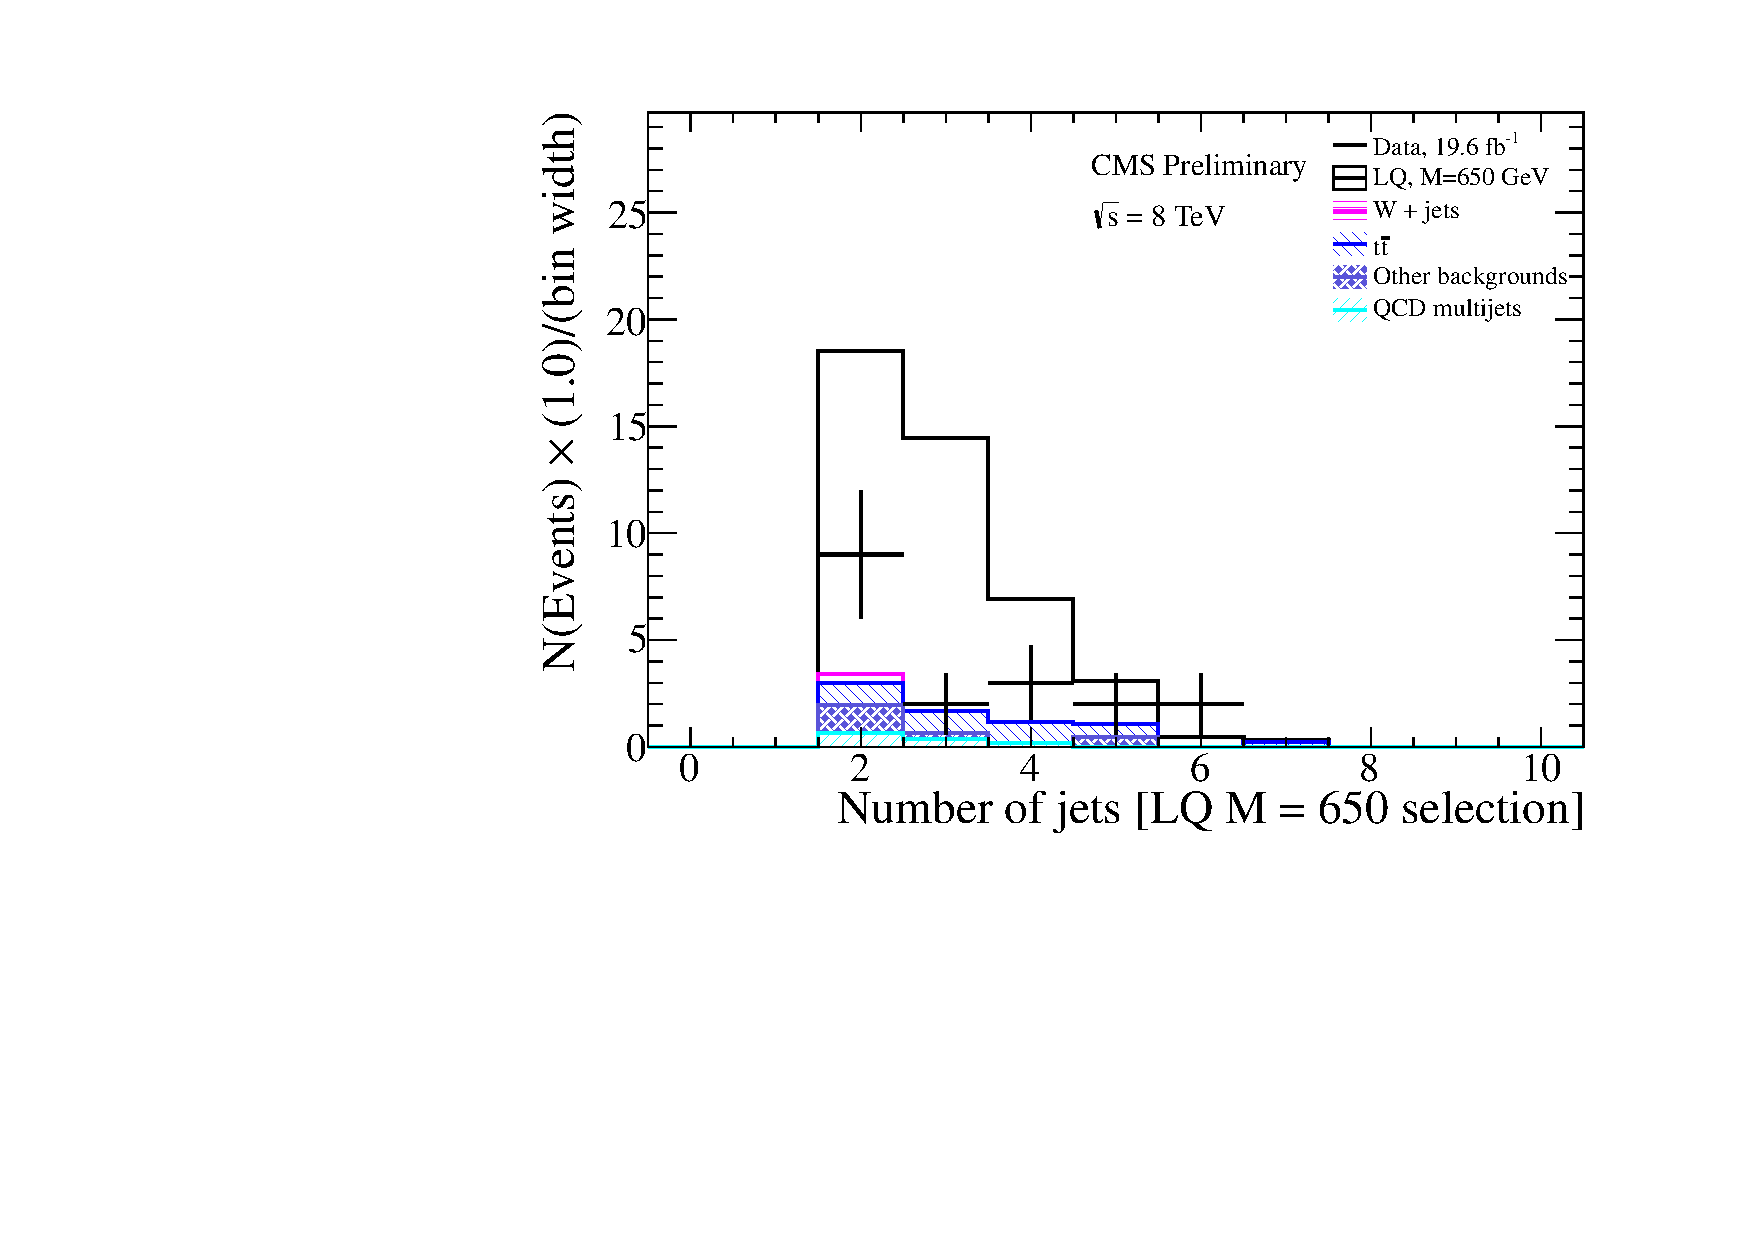
\includegraphics[width=0.8\textwidth]{fig/enu/extra/nJets_LQ650_enujj.pdf}
\end{column}
\end{columns}
\end{frame}
\subsection{\eejj N-1 plots}
\label{sec-1-12}
\begin{frame}
\frametitle{\eejj N-1 plots: M(LQ) = 450 selection}
\label{sec-1-12-1}
\begin{columns} % Columns
\label{sec-1-12-1-1}
\begin{column}{0.55\textwidth}
%% 1st column
\label{sec-1-12-1-1-1}
%% 1st block in 1st column
\label{sec-1-12-1-1-1-1}

\centering
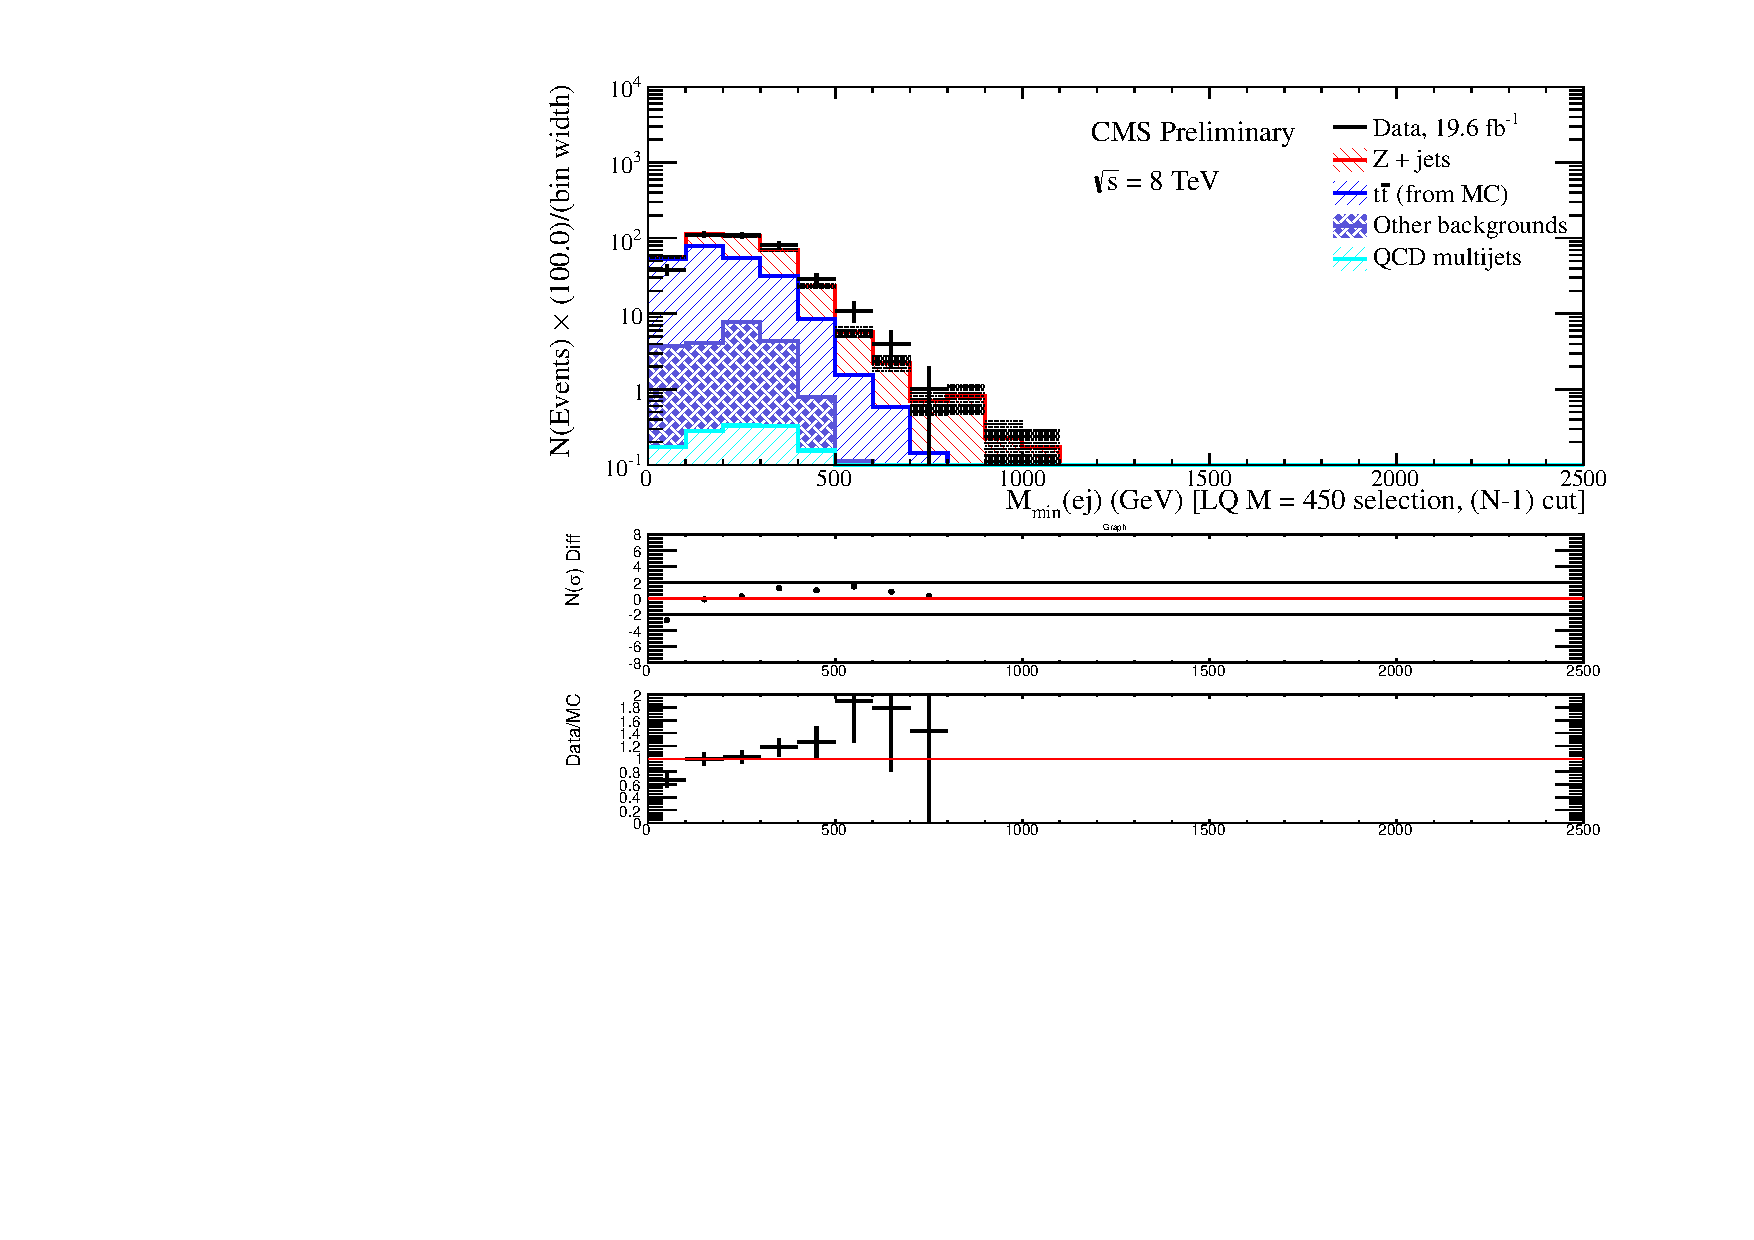
\includegraphics[width=0.8\textwidth]{fig/ee/nMinus1/Mej_selected_min_StAndMeeLQ450_eejj.pdf}
%% 2nd block in 1st column
\label{sec-1-12-1-1-1-2}

\centering
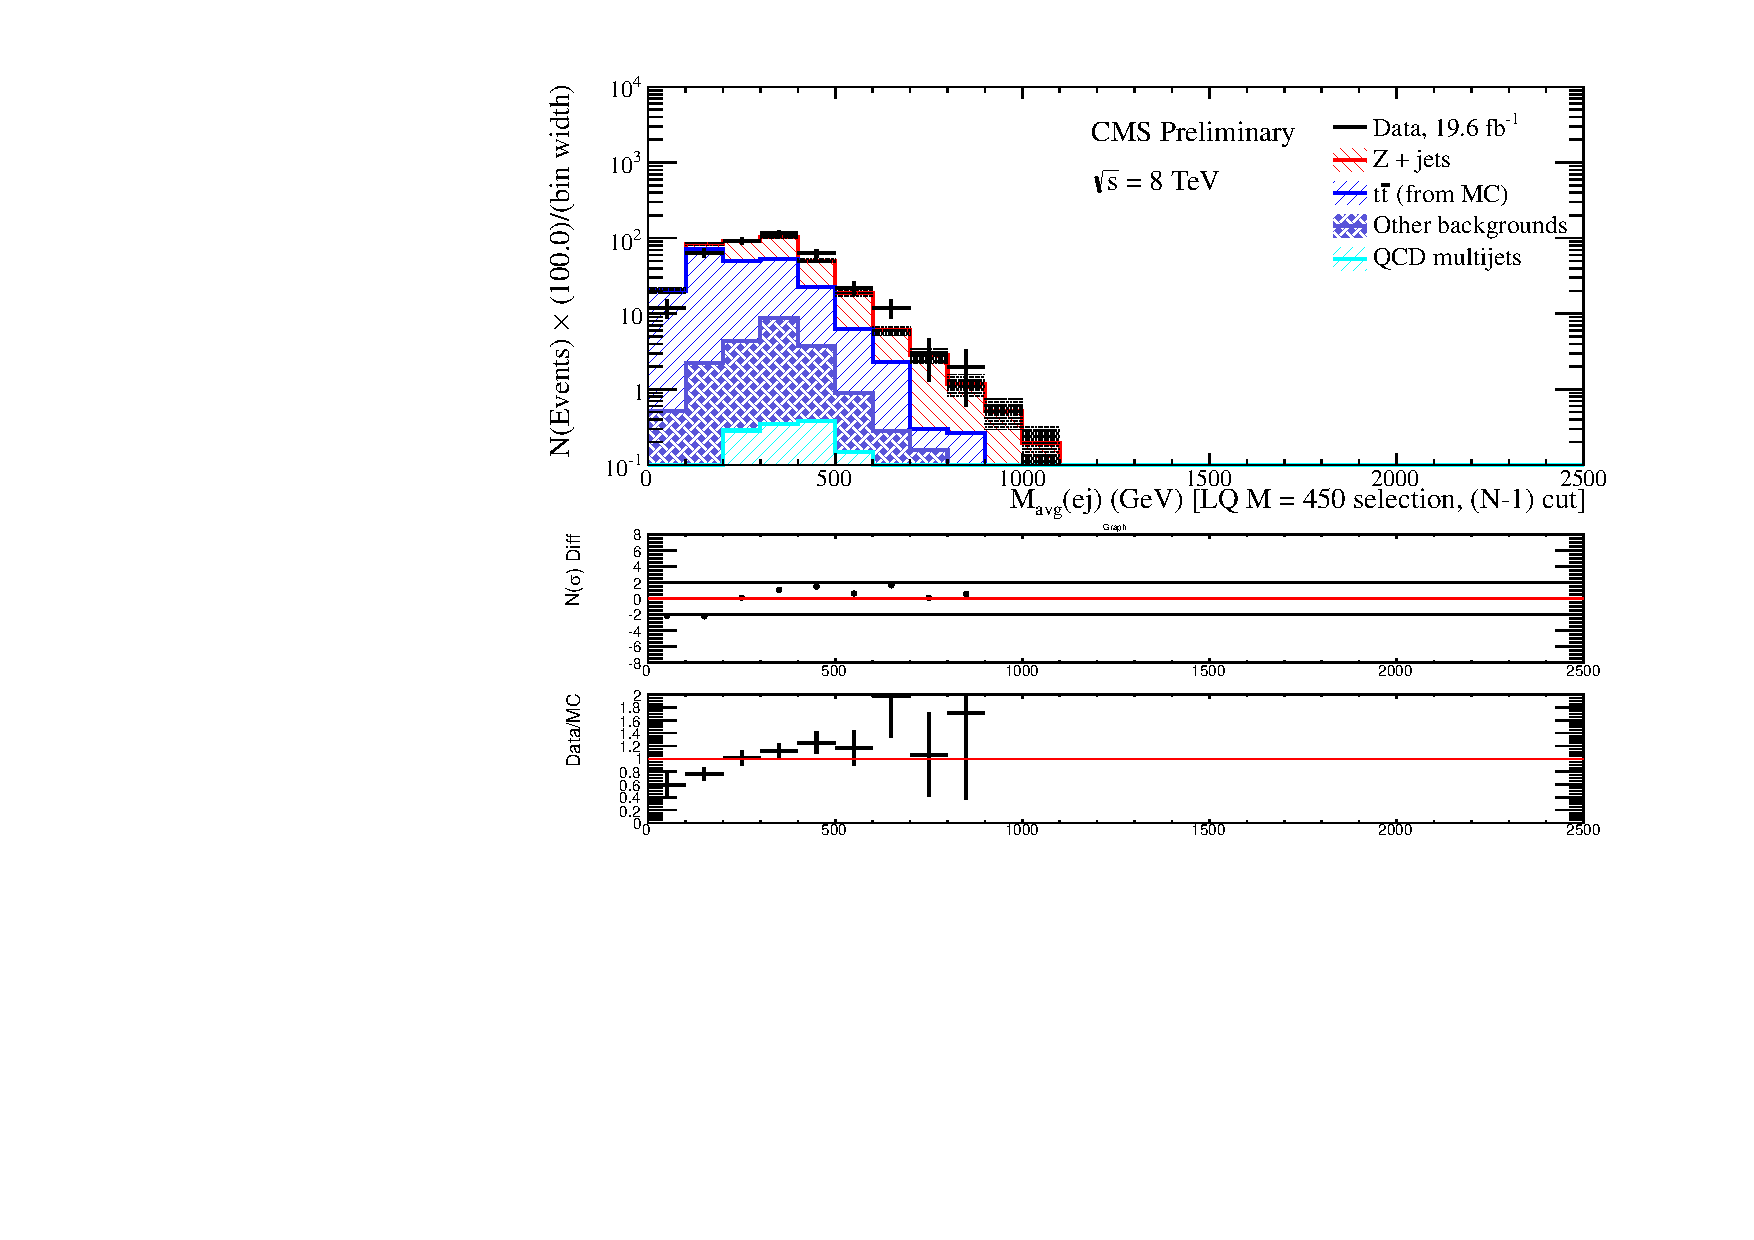
\includegraphics[width=0.8\textwidth]{fig/ee/nMinus1/Mej_selected_avg_StAndMeeLQ450_eejj.pdf}
\end{column}
\begin{column}{0.55\textwidth}
%% 2nd column
\label{sec-1-12-1-1-2}
%% 1st block in 2nd column
\label{sec-1-12-1-1-2-1}

\centering
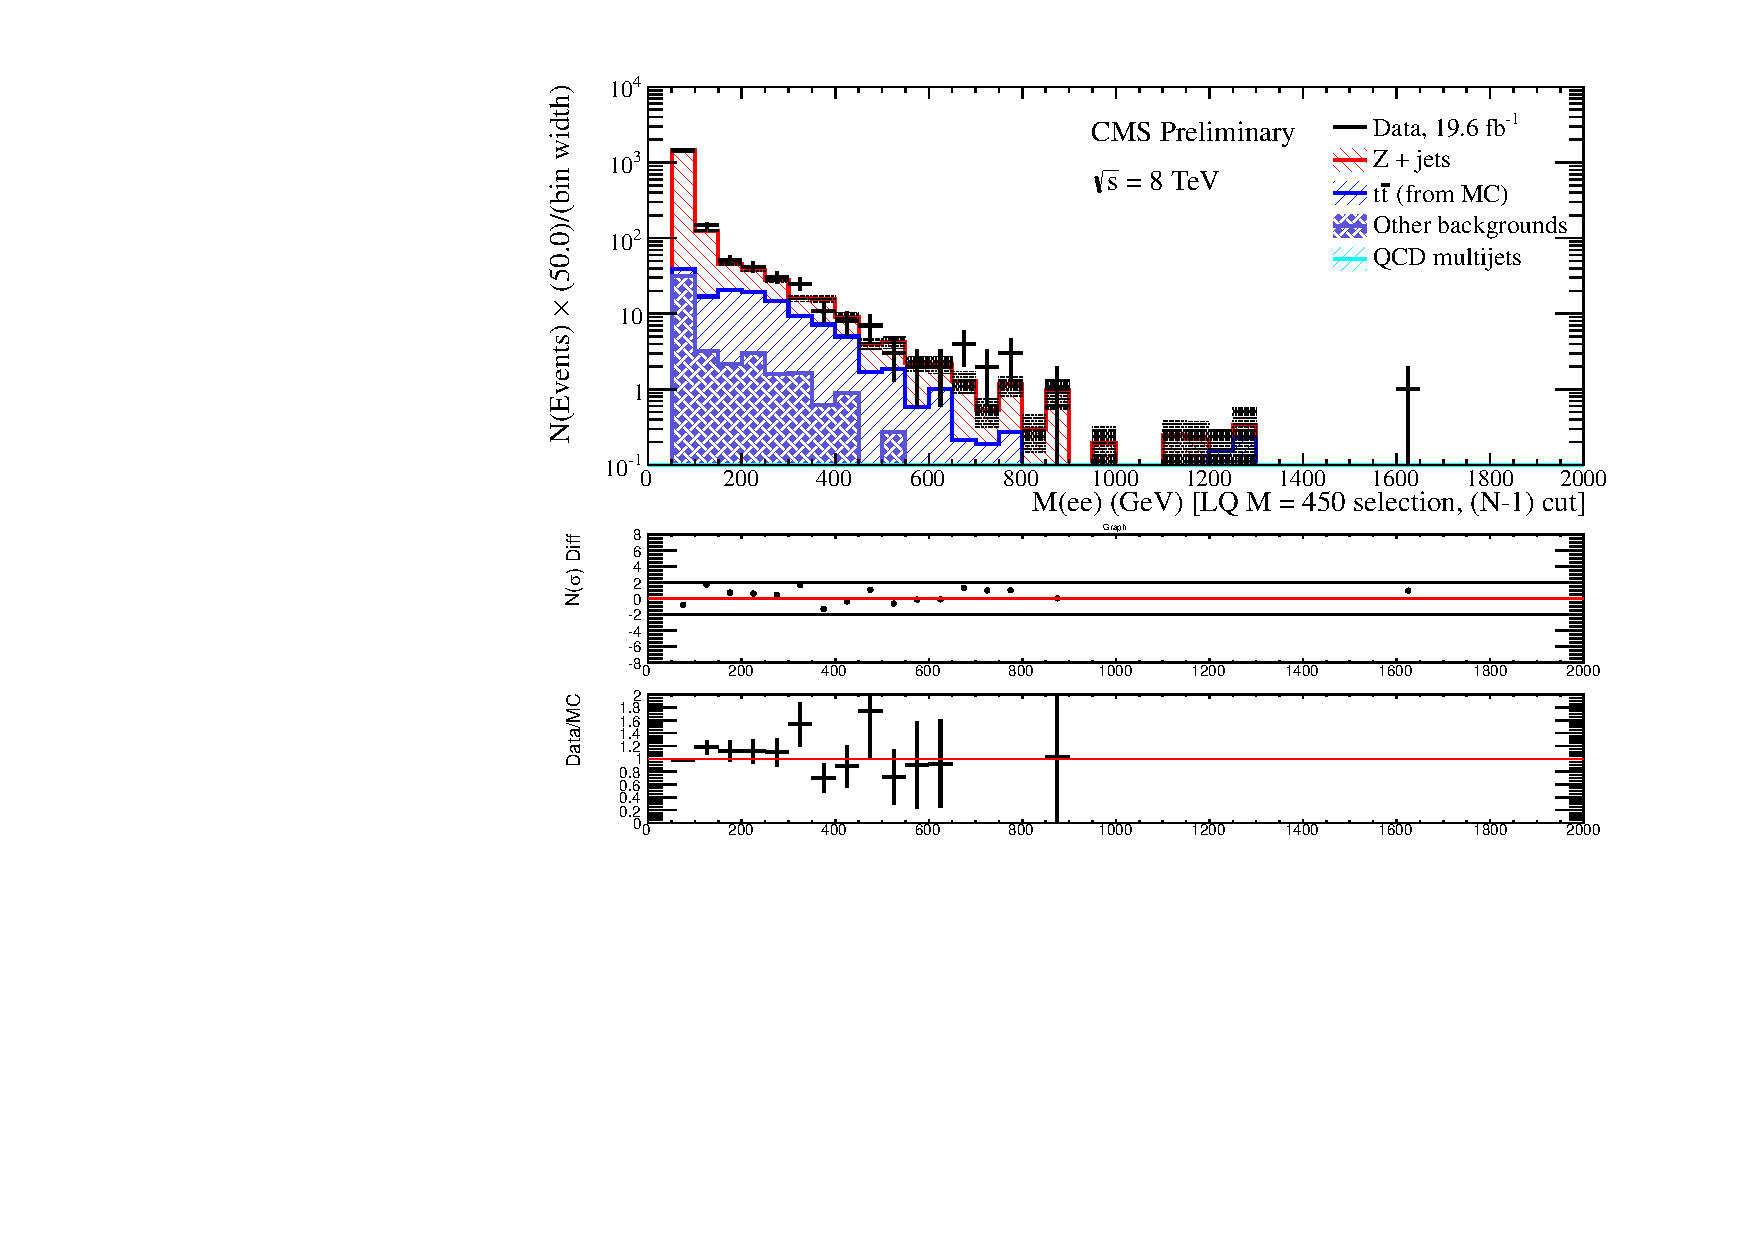
\includegraphics[width=0.8\textwidth]{fig/ee/nMinus1/Mee_StAndMejLQ450_eejj.pdf}
%% 2nd block in 2nd column
\label{sec-1-12-1-1-2-2}


\centering
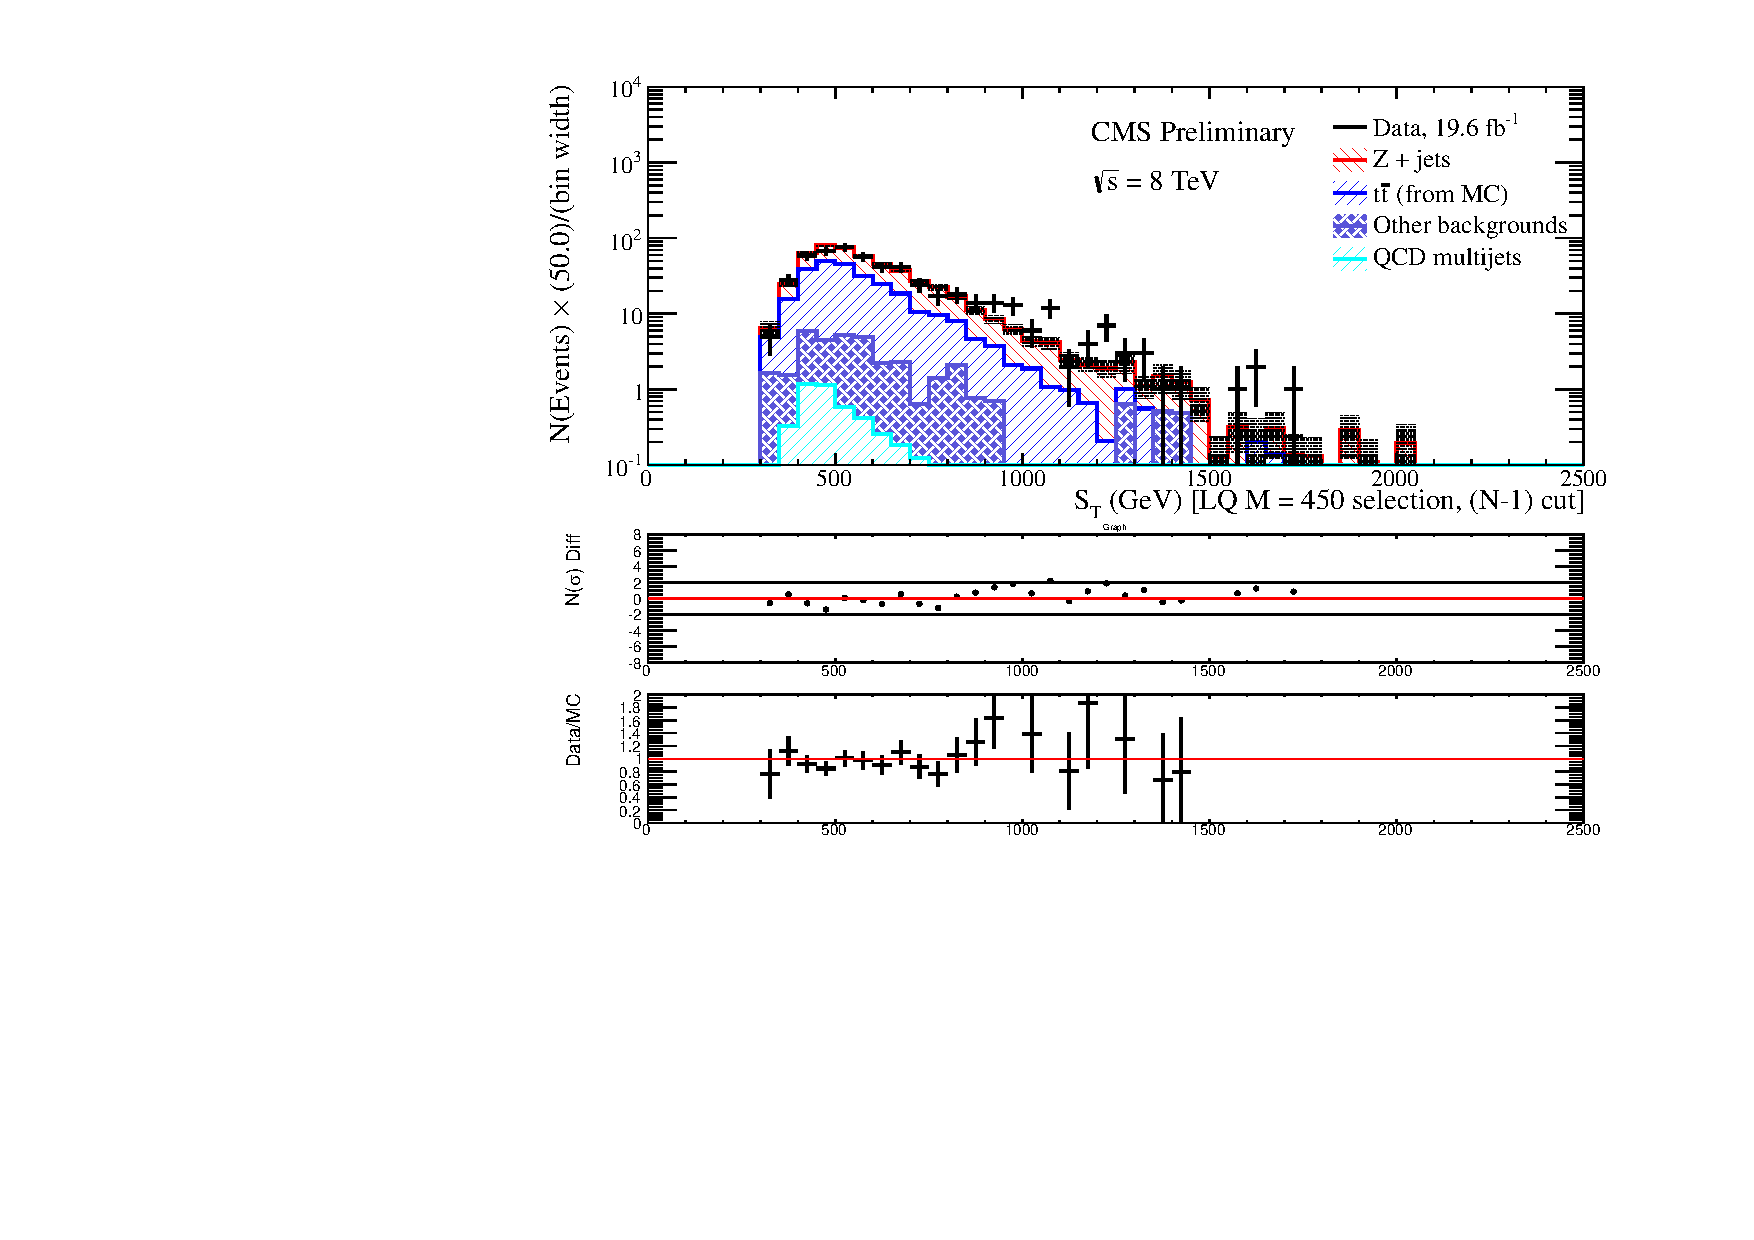
\includegraphics[width=0.8\textwidth]{fig/ee/nMinus1/sT_eejj_MeeAndMejLQ450_eejj.pdf}
\end{column}
\end{columns}
\end{frame}
\begin{frame}
\frametitle{\eejj N-1 plots: M(LQ) = 650 selection}
\label{sec-1-12-2}
\begin{columns} % Columns
\label{sec-1-12-2-1}
\begin{column}{0.55\textwidth}
%% 1st column
\label{sec-1-12-2-1-1}
%% 1st block in 1st column
\label{sec-1-12-2-1-1-1}

\centering
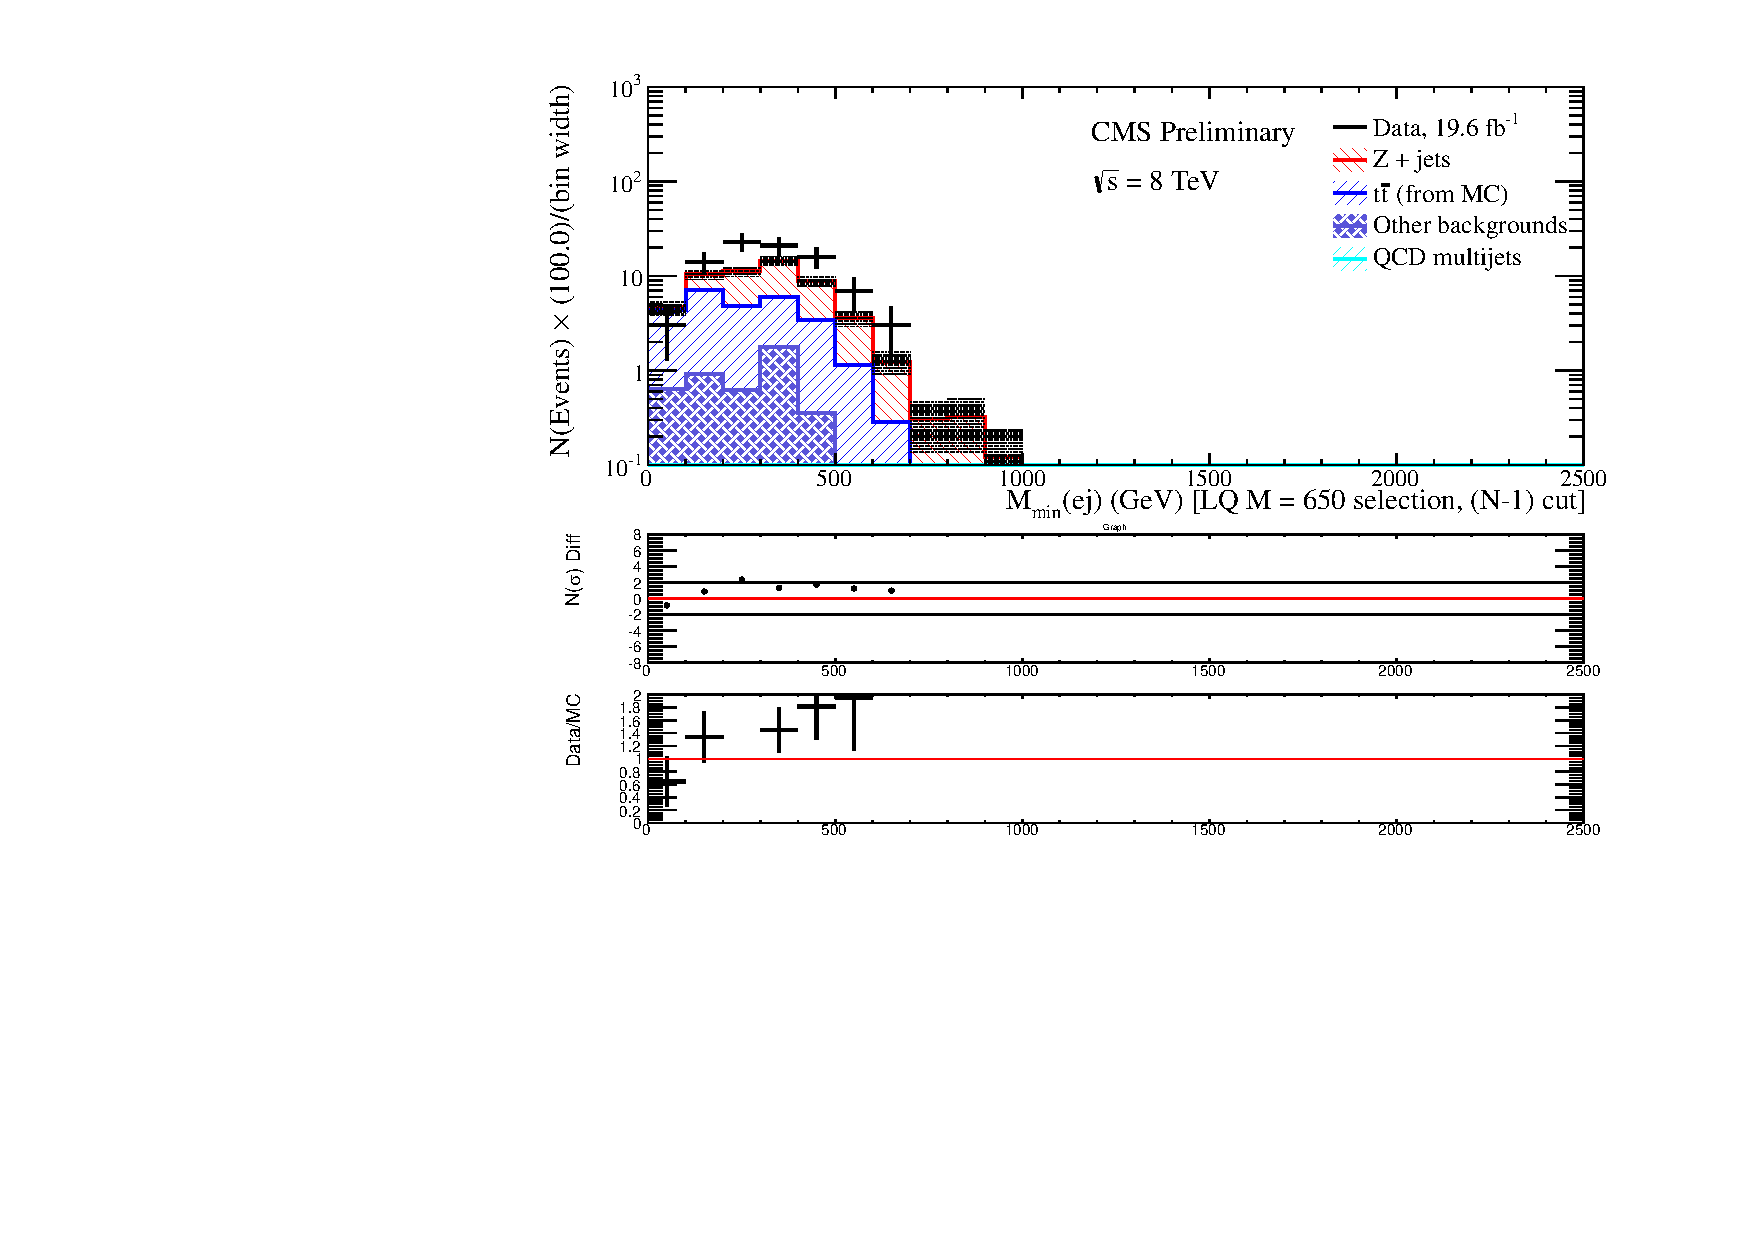
\includegraphics[width=0.8\textwidth]{fig/ee/nMinus1/Mej_selected_min_StAndMeeLQ650_eejj.pdf}
%% 2nd block in 1st column
\label{sec-1-12-2-1-1-2}

\centering
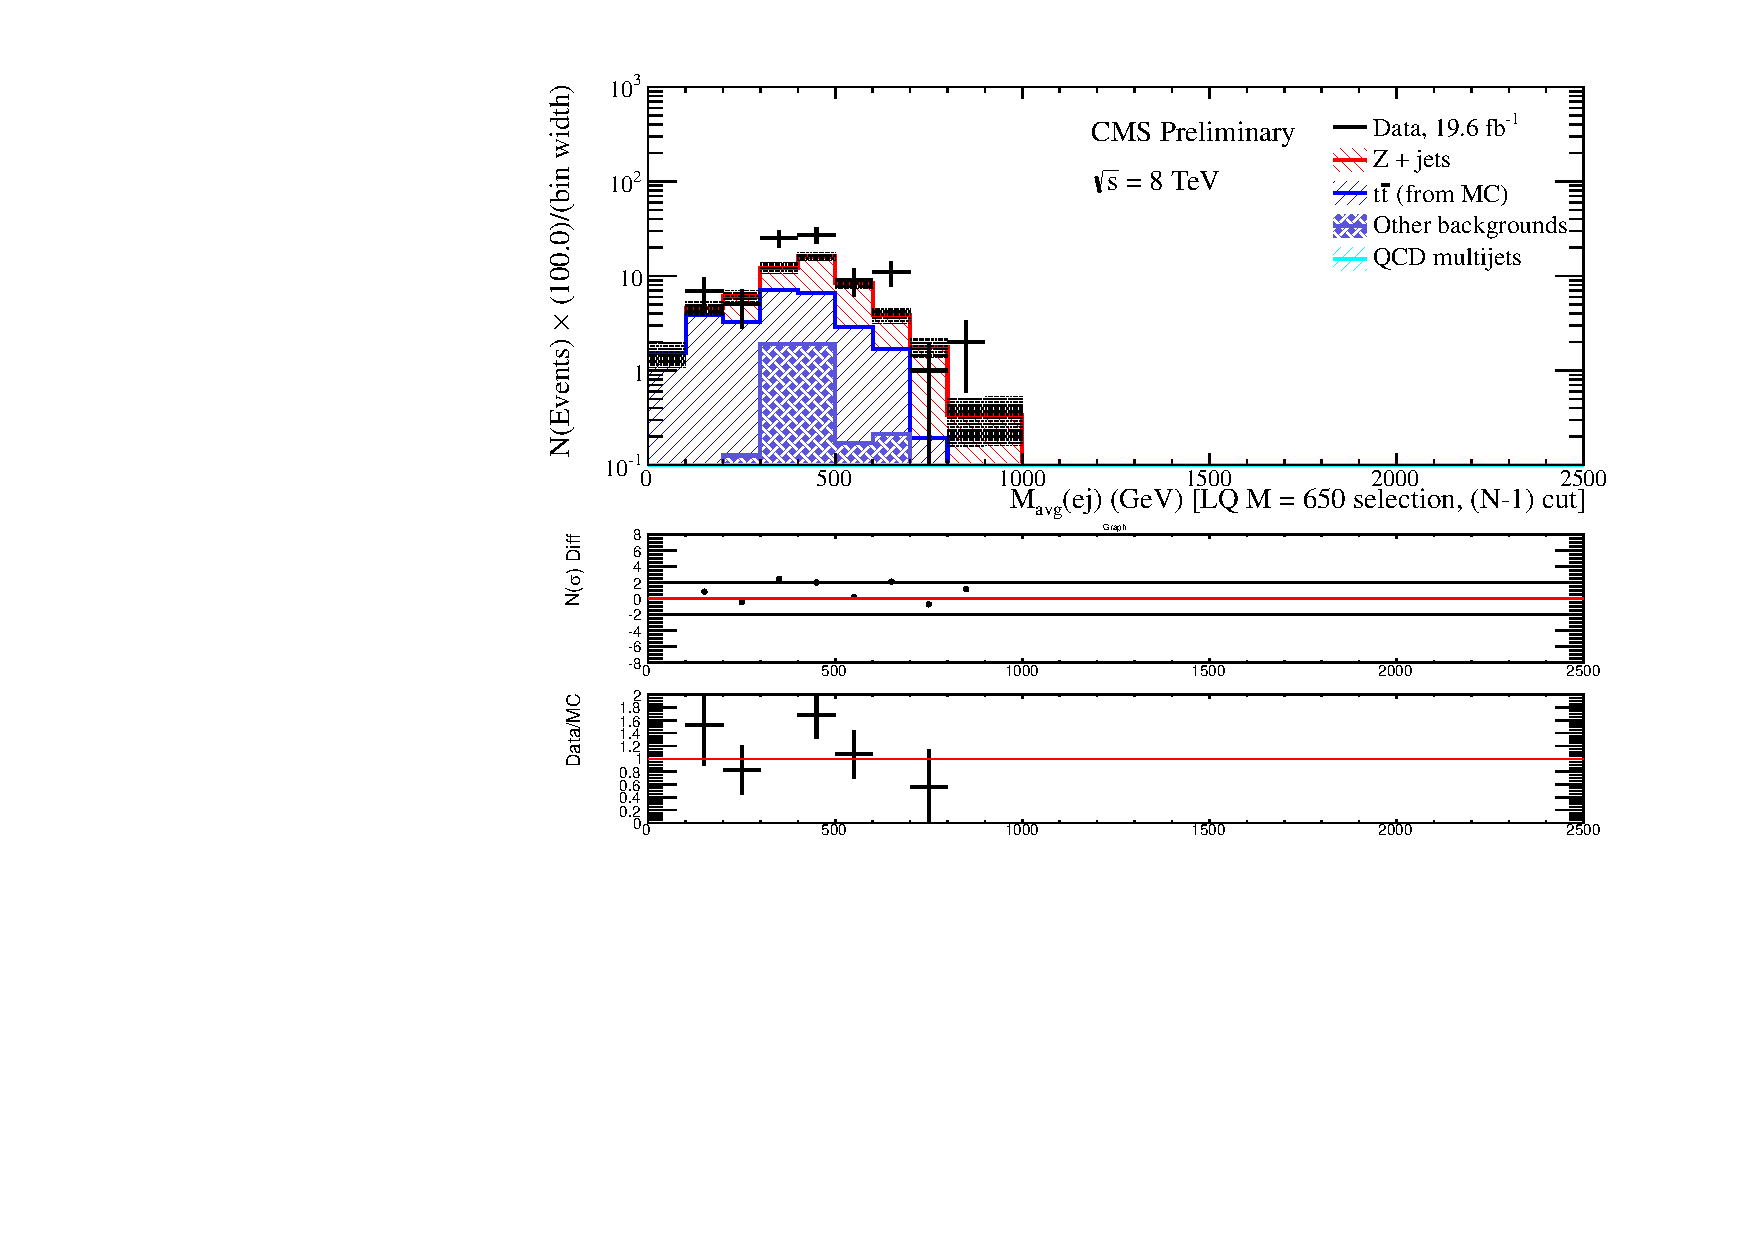
\includegraphics[width=0.8\textwidth]{fig/ee/nMinus1/Mej_selected_avg_StAndMeeLQ650_eejj.pdf}
\end{column}
\begin{column}{0.55\textwidth}
%% 2nd column
\label{sec-1-12-2-1-2}
%% 1st block in 2nd column
\label{sec-1-12-2-1-2-1}

\centering
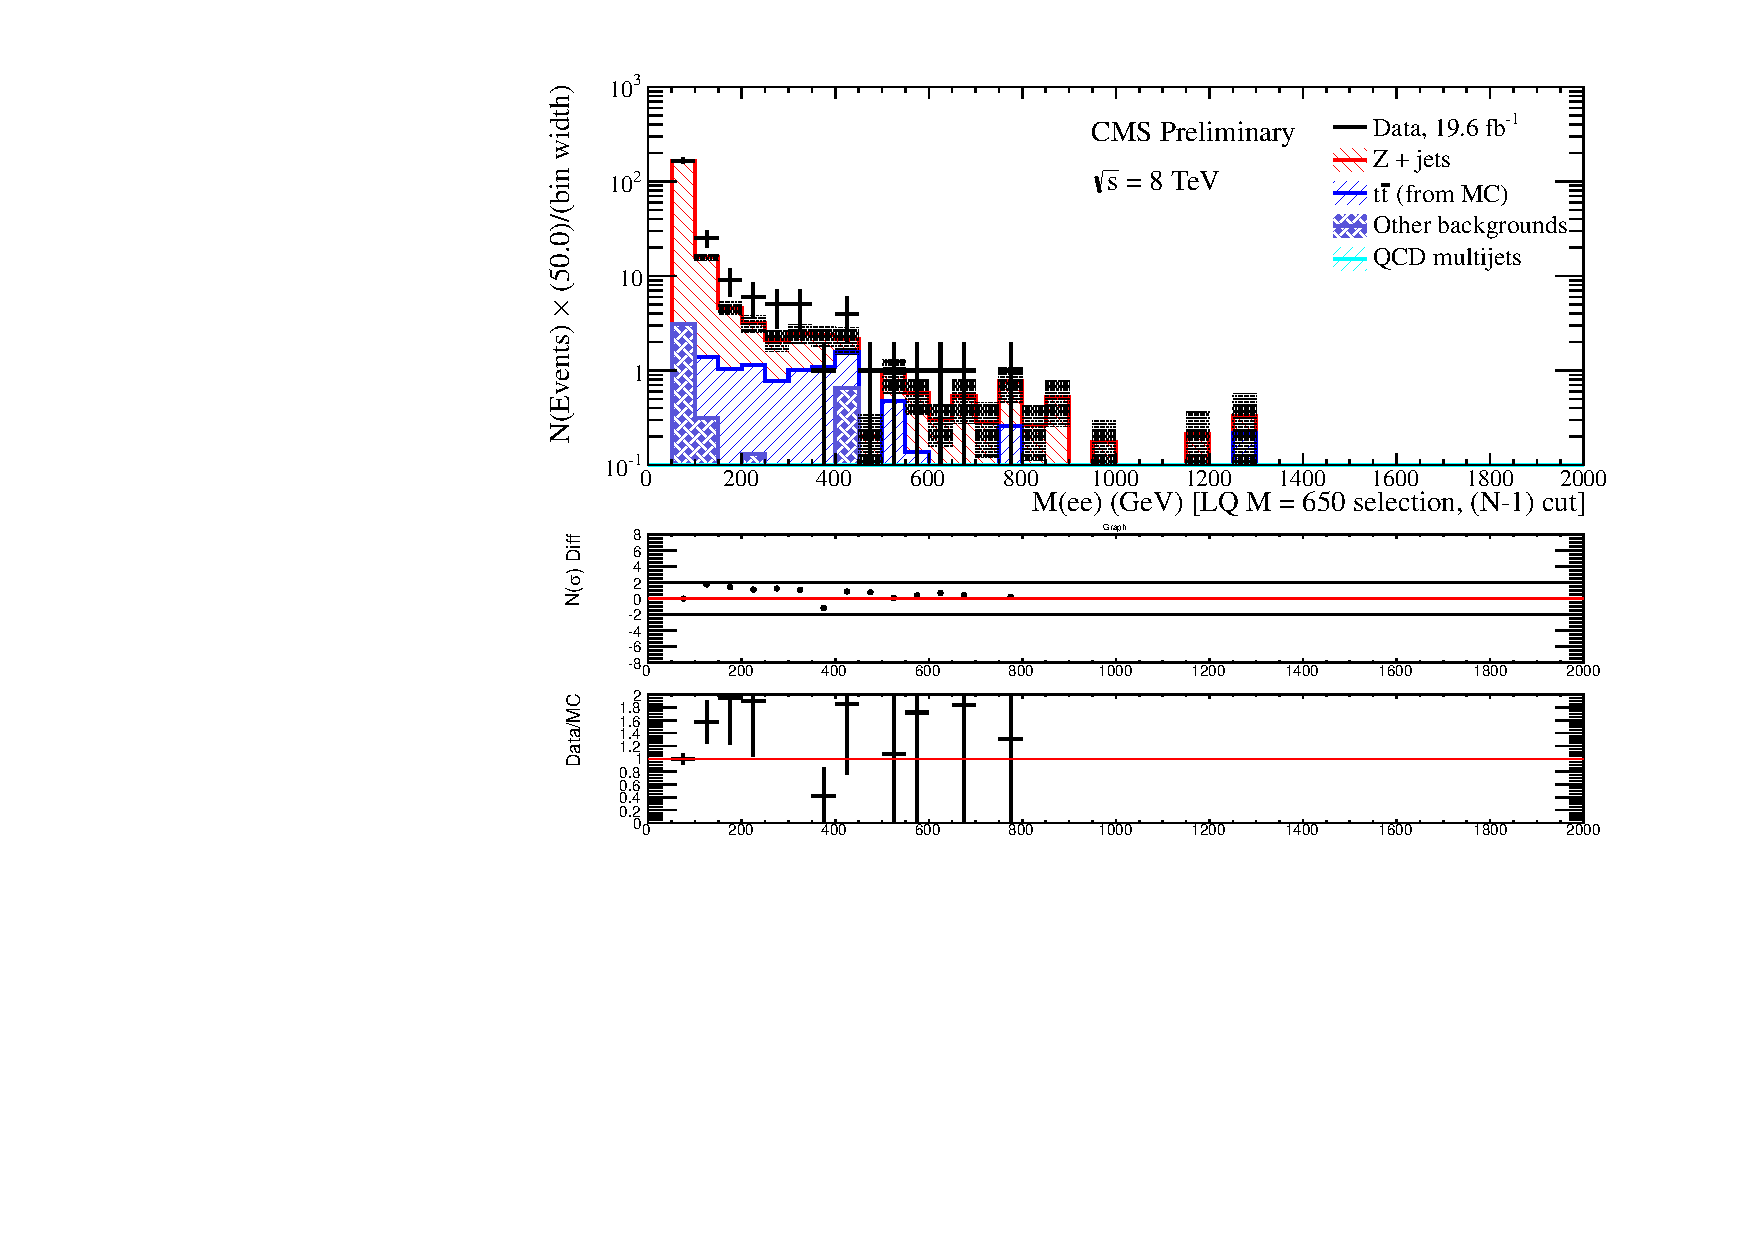
\includegraphics[width=0.8\textwidth]{fig/ee/nMinus1/Mee_StAndMejLQ650_eejj.pdf}
%% 2nd block in 2nd column
\label{sec-1-12-2-1-2-2}


\centering
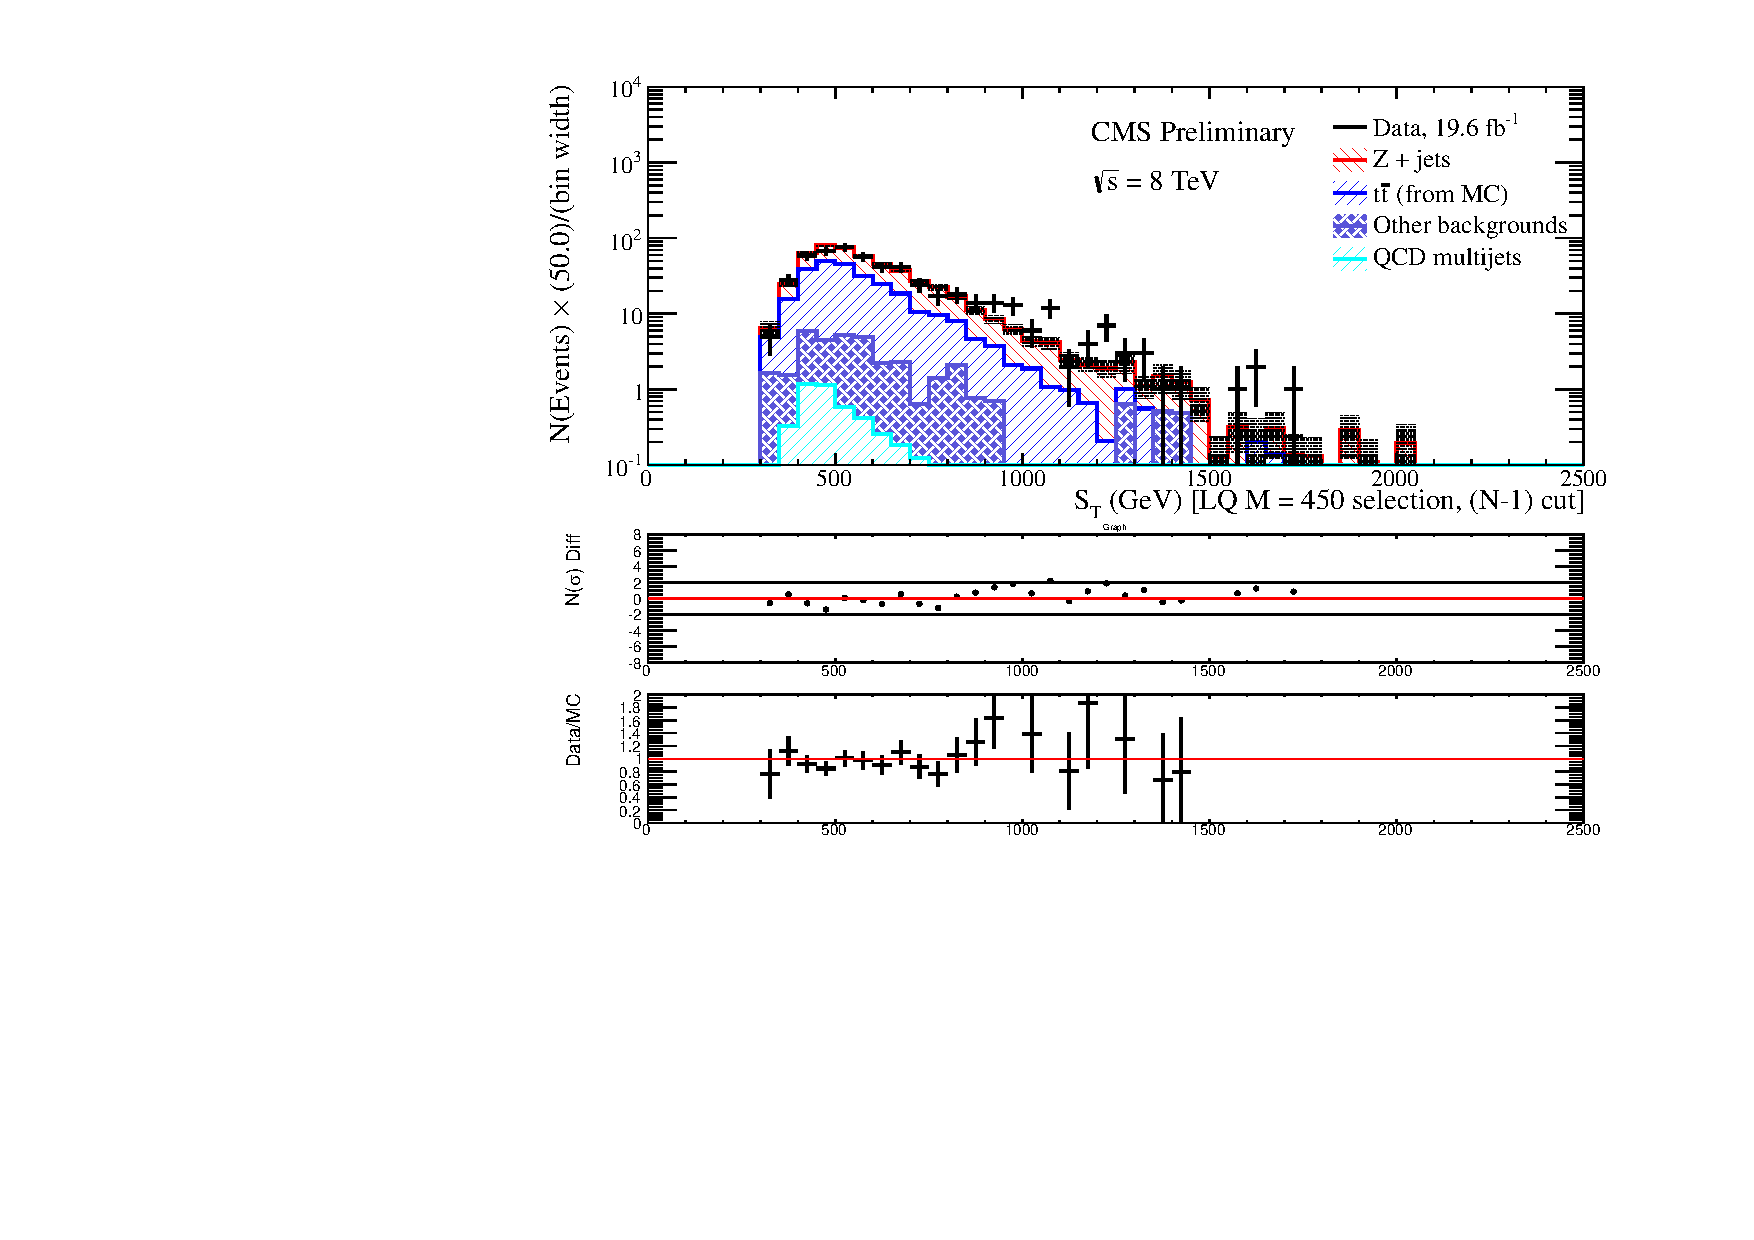
\includegraphics[width=0.8\textwidth]{fig/ee/nMinus1/sT_eejj_MeeAndMejLQ450_eejj.pdf}
\end{column}
\end{columns}
\end{frame}
\subsection{\enujj N-1 plots}
\label{sec-1-13}
\begin{frame}
\frametitle{\enujj N-1 plots: M(LQ) = 450 selection}
\label{sec-1-13-1}
\begin{columns} % Columns
\label{sec-1-13-1-1}
\begin{column}{0.55\textwidth}
%% 1st column
\label{sec-1-13-1-1-1}
%% 1st block in 1st column
\label{sec-1-13-1-1-1-1}

\centering
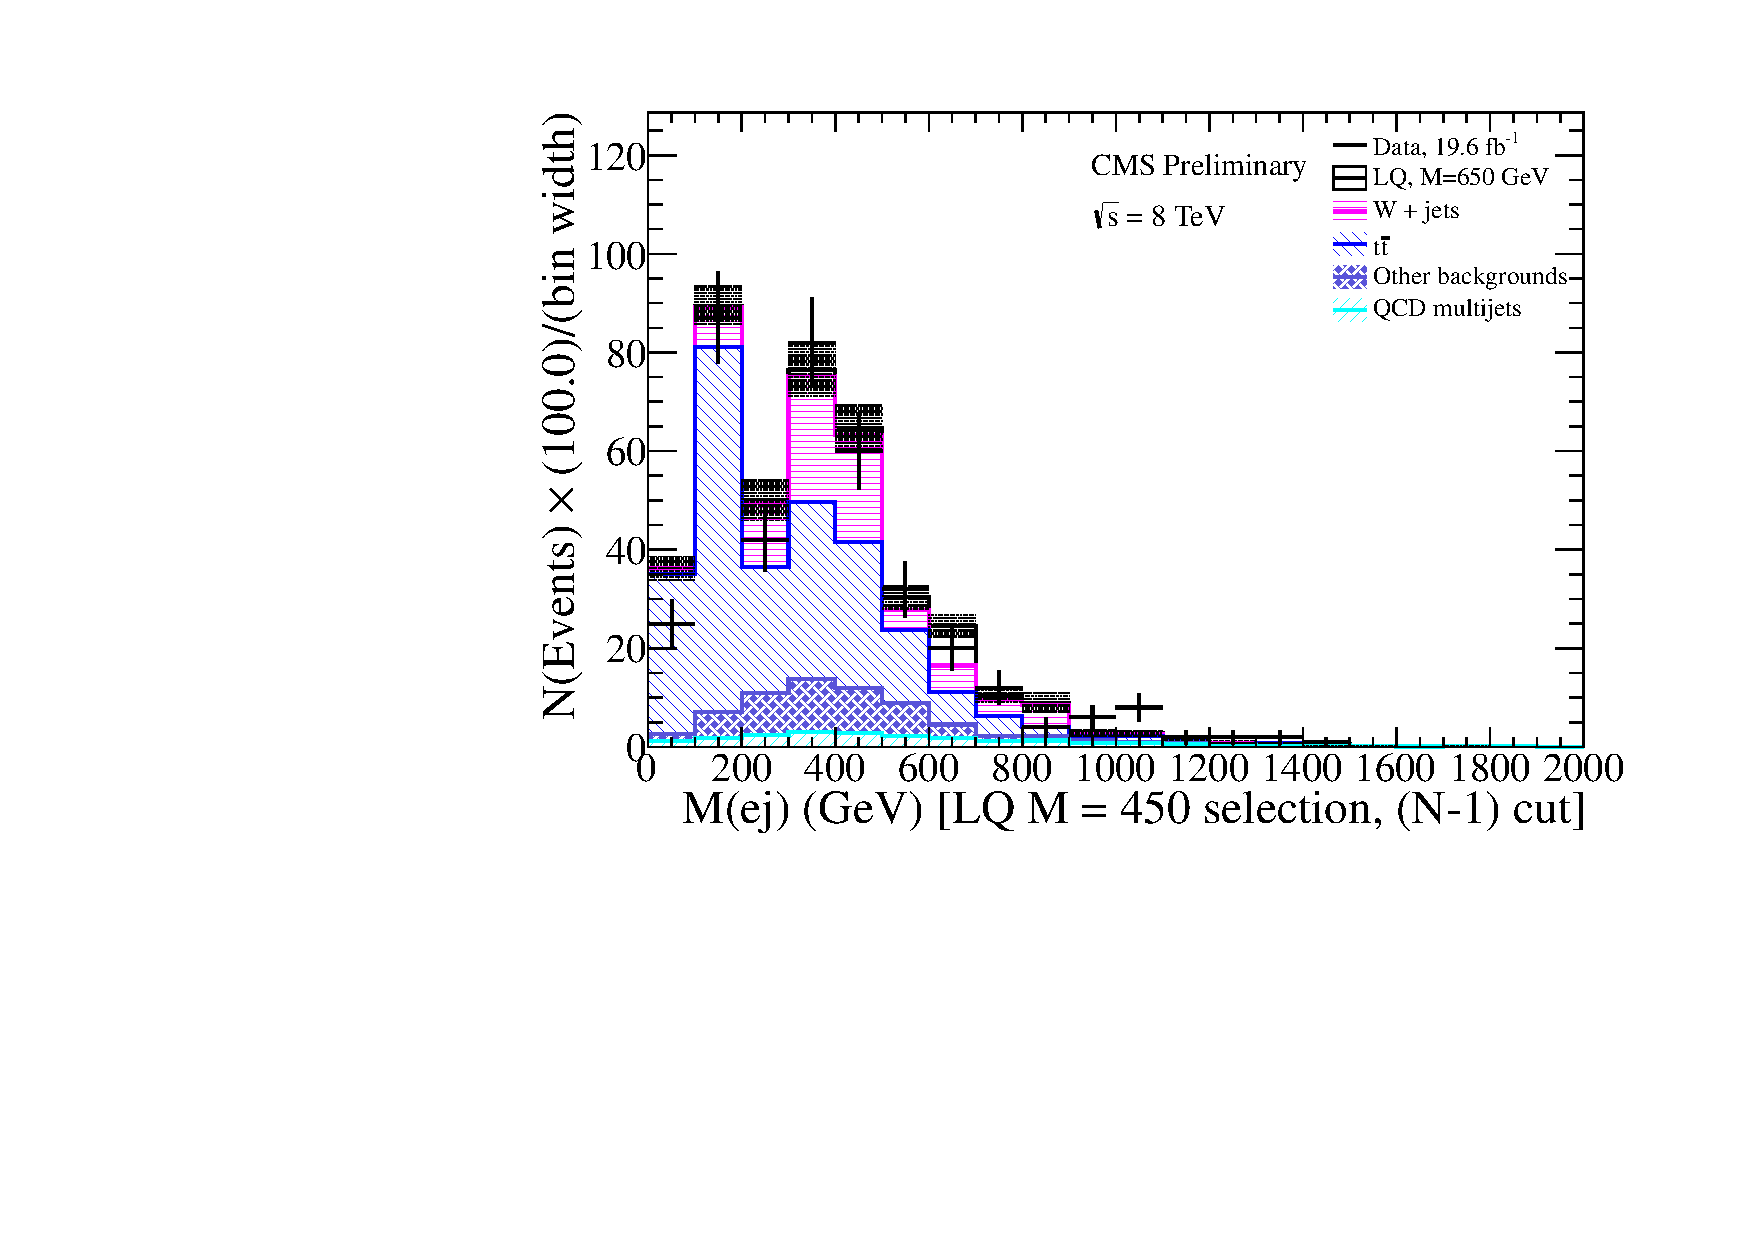
\includegraphics[width=0.8\textwidth]{fig/enu/nMinus1/Mej_stAndMtAndMetLQ450_enujj.pdf}
%% 2nd block in 1st column
\label{sec-1-13-1-1-1-2}

\centering
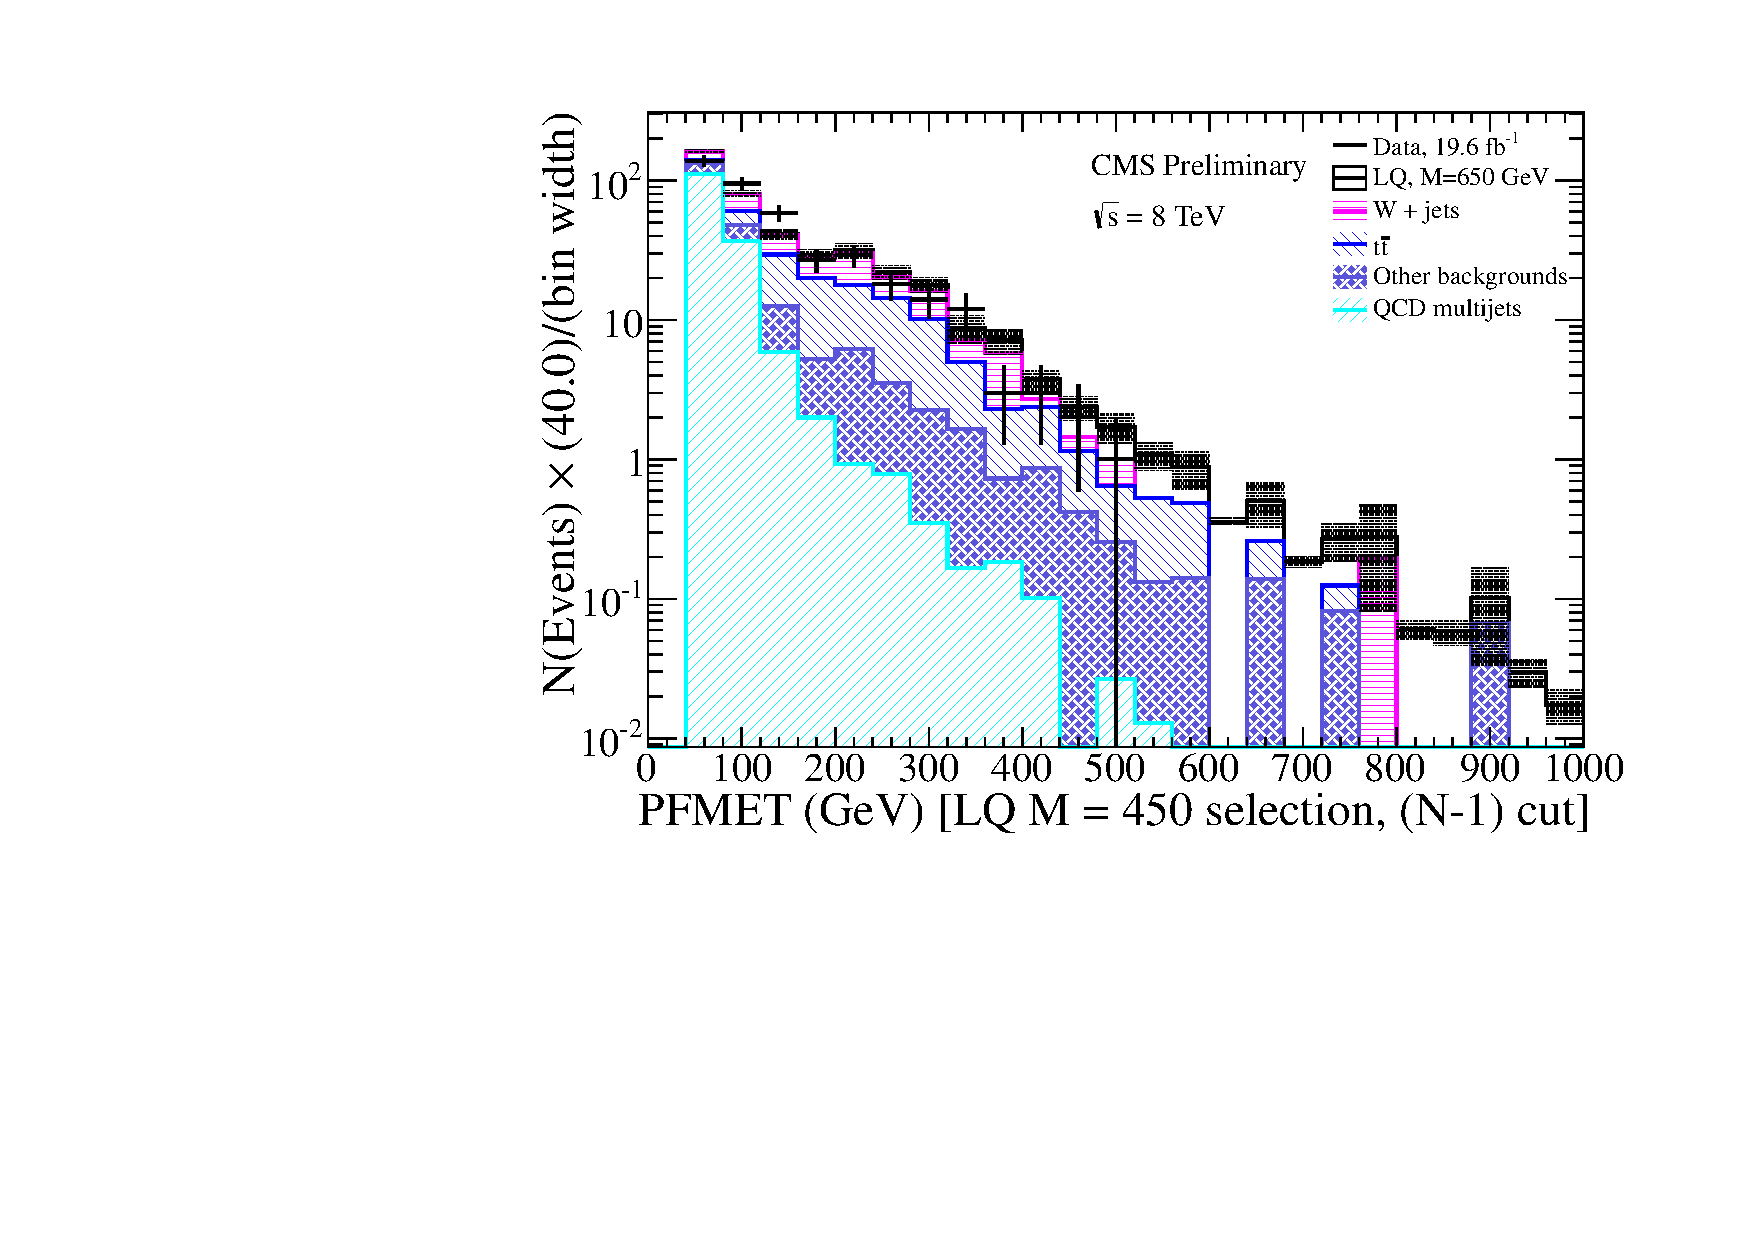
\includegraphics[width=0.8\textwidth]{fig/enu/nMinus1/MET_stAndMtAndMejLQ450_enujj.pdf}
\end{column}
\begin{column}{0.55\textwidth}
%% 2nd column
\label{sec-1-13-1-1-2}
%% 1st block in 2nd column
\label{sec-1-13-1-1-2-1}

\centering
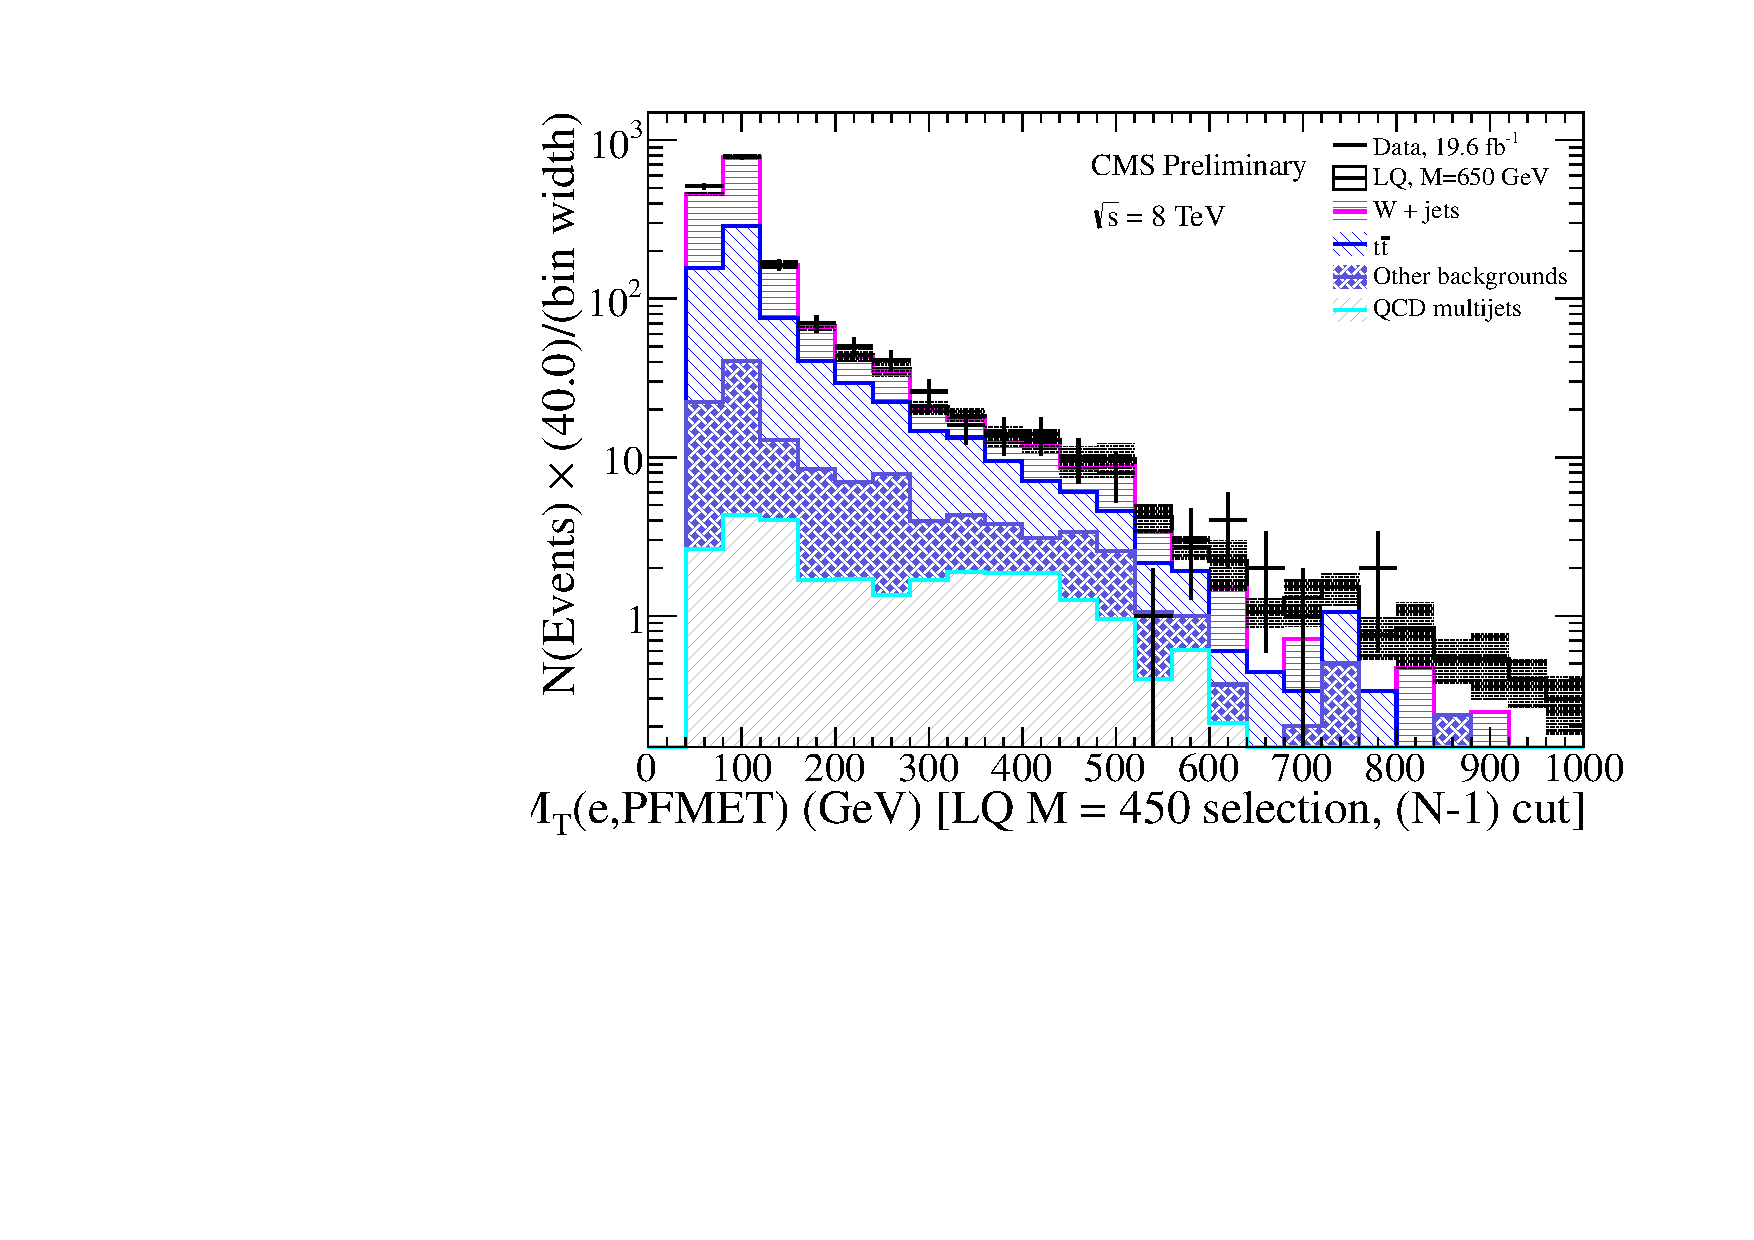
\includegraphics[width=0.8\textwidth]{fig/enu/nMinus1/MTenu_stAndMetAndMejLQ450_enujj.pdf}
%% 2nd block in 2nd column
\label{sec-1-13-1-1-2-2}

\centering
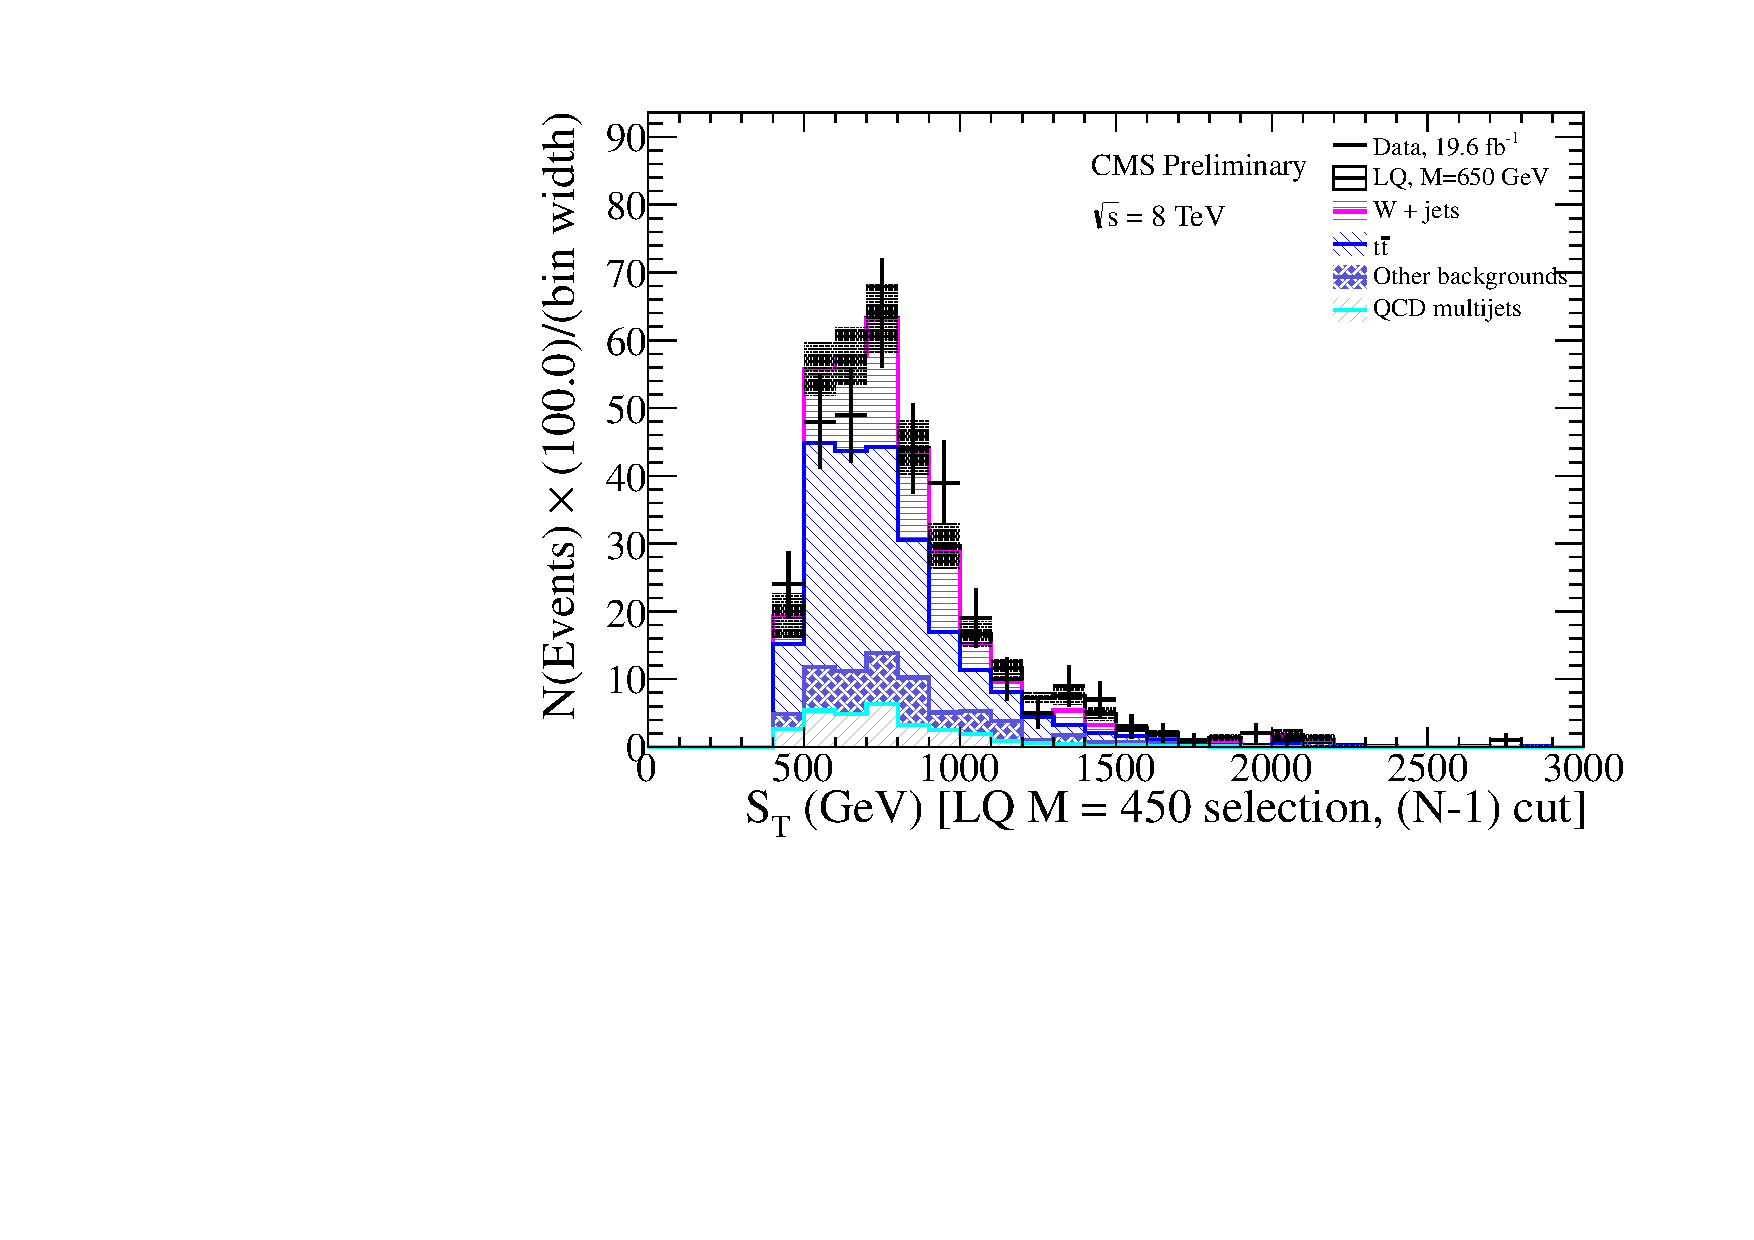
\includegraphics[width=0.8\textwidth]{fig/enu/nMinus1/ST_mtAndMetAndMejLQ450_enujj.pdf}
\end{column}
\end{columns}
\end{frame}
\begin{frame}
\frametitle{\enujj N-1 plots: M(LQ) = 650 selection}
\label{sec-1-13-2}
\begin{columns} % Columns
\label{sec-1-13-2-1}
\begin{column}{0.55\textwidth}
%% 1st column
\label{sec-1-13-2-1-1}
%% 1st block in 1st column
\label{sec-1-13-2-1-1-1}

\centering
\includegraphics[width=0.8\textwidth]{fig/enu/nMinus1/Mej_stAndMtAndMetLQ650_enujj.pdf}
%% 2nd block in 1st column
\label{sec-1-13-2-1-1-2}

\centering
\includegraphics[width=0.8\textwidth]{fig/enu/nMinus1/MET_stAndMtAndMejLQ650_enujj.pdf}
\end{column}
\begin{column}{0.55\textwidth}
%% 2nd column
\label{sec-1-13-2-1-2}
%% 1st block in 2nd column
\label{sec-1-13-2-1-2-1}

\centering
\includegraphics[width=0.8\textwidth]{fig/enu/nMinus1/MTenu_stAndMetAndMejLQ650_enujj.pdf}
%% 2nd block in 2nd column
\label{sec-1-13-2-1-2-2}

\centering
\includegraphics[width=0.8\textwidth]{fig/enu/nMinus1/ST_mtAndMetAndMejLQ650_enujj.pdf}
\end{column}
\end{columns}
\end{frame}

\end{document}
